\documentclass{report}

\usepackage{color}

% Index
\usepackage{makeidx}
\makeindex
\newcommand\INDEX[1]{{#1}\index{#1}}

% Switch mostly to Helvetica
\usepackage{helvet}
\usepackage{sectsty}
\allsectionsfont{\sffamily}
\renewcommand*\figurename{\sffamily Figure}
\renewcommand*\tablename{\sffamily Table}

% Source-Code Listings (Version 0.2)
\usepackage{listings}
%\usepackage{styles/lstpatch}
\lstloadlanguages{C,C++,csh,Perl}
\lstset{language=C++}
\lstset{basicstyle=\sffamily,frame=trlb}
\lstset{captionpos=b,xleftmargin=0cm,xrightmargin=0cm}
\lstset{morekeywords={record},keywordstyle=\bfseries}
\renewcommand*\lstlistingname{\sffamily Listing}

% PDF Support
\definecolor{rltred}{rgb}{0.75,0,0}
\definecolor{rltgreen}{rgb}{0,0.5,0}
\definecolor{rltblue}{rgb}{0,0,0.75}
% Create a new ifpdf to allow conditional translation w/ and w/o PDF:
%\newif\ifpdf
%\ifx\pdfoutput\undefined
%    \pdffalse          % we are not running PDFLaTeX
%\else
\pdfoutput=1       % we are running PDFLaTeX
%\pdftrue
%\fi
%\ifpdf
% PDF-only stuff
\usepackage[pdftex,
        colorlinks=true,
        urlcolor=rltblue,       % \href{...}{...} external (URL)
        filecolor=rltgreen,     % \href{...} local file
        linkcolor=rltred,       % \ref{...} and \pageref{...}
        pdftitle={Channel Archiver Manual},
        pdfauthor={Kay-Uwe Kasemir},
        pdfsubject={EPICS Channel Archiver},
        pdfkeywords={EPICS, Archiver, ChannelAccess},
        pagebackref,
        pdfpagemode=None,
        bookmarksopen=true]{hyperref}
\usepackage[pdftex]{graphicx}
%\else
% Non-PDF Stuff
%\usepackage[dvips]{graphicx}
%\fi

%\DeclareGraphicsExtensions{.png}

% InsertImage{width=...,height=...}{image basename}
%% Trick: The minipage aligns top/center/bottom
%% by aligning the baseline.
%% With only the \includegraphics, that single line
%% would be the baseline and thus [t] == [b].
%% By adding zero-sized lines above and below \includegraphics,
%% we can actually use [t] and [b].
%% [From TUGBoat 17(1996)3 ]

\newcommand\InsertImage[2]{
  \vspace{-\baselineskip}
  \includegraphics[#1]{#2}
  \par\vspace{0pt}
}

\definecolor{red}{rgb}{0.5,0,0}
\newcommand\NOTE[0]{\noindent{\bfseries\color{red}NOTE:~}}

\hyphenation{re-cords phys-ics Ar-chive-En-gine Ar-chive-Da-ta-Ser-ver}

\begin{document}
\sffamily
\title{\Huge Channel Archiver Manual\\[1cm]
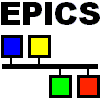
\includegraphics[width=3cm]{images/logo101.png}
}
\date{\today,\\ for R3.14.4 and higher}
\maketitle
\newpage

\pagestyle{empty}

\section*{Involvements}
Bob Dalesio designed the original index file, data file layout,
and implemented the first prototype.\\
From then on, the following people have been involved at one
time or another:\\
\begin{center}
Thomas Birke,\\
Sergei Chevtsov,\\
Kay-Uwe Kasemir,\\ 
Chris Larrieu,\\
Greg Lawson,\\
Craig McChesney,\\
Peregrine McGehee,\\
Nick Pattengale,\\
Ernest Williams,\\
Noboru Yamamoto.
\end{center}

\section*{No Warranty}
Although the programs and procedures described in this manual are
meant to be helpful instruments for archiving, maintaining and
retrieving control system data, there is no warranty, either expressed
or implied, including, but not limited to, fitness for a particular
purpose. The entire risk as to the quality and performance of the
programs and procedures is with you.  Should the programs or
procedures prove defective, you assume the cost of all necessary
servicing, repair or correction.

In no event will anybody, including the persons listed above, be
liable to you for damages, including any general, special, incidental
or consequential damages arising out of the use or inability to use
the programs (including but not limited to loss of data or data being
rendered inaccurate or losses sustained by you or third parties or a
failure of the programs to operate with any other programs).

\newpage

\pagenumbering{roman}
\tableofcontents
\newpage
\pagestyle{headings}
\pagenumbering{arabic}
\setcounter{page}{1}

\chapter{Overview}
The Channel Archiver is an archiving toolset for the Experimental Physics
and Industrial Control System, \INDEX{EPICS}~\cite{ANLweb}.
It can archive any value that is available via \INDEX{ChannelAccess}
(\INDEX{CA}), the EPICS network protocol~\cite{hill89}.
We use the term ``archiver'' whenever we refer to the collection of
programs which allow us to take samples, place them into some storage
and retrieve them again.

\section{Audience}
Casual users will probably only need to know how to run the ``Java Archive
Viewer'' program and read its online help ---
none of which is part of this manual, except for a brief glimpse in 
section \ref{sec:javaclient}.
They may refer to the background information in chapter
\ref{ch:background} for a general understanding of the archiver.

Engineers who configure archive engines will need to be familiar with
the fundamentals up to and including the ArchiveEngine description in
chapter \ref{sec:engine}. They also need to understand the Example
Setup, chapter \ref{ch:examplesetup}, unless their site uses a
different setup which is then described in site-specific
documentation.

If you are stuck with installing and maintaining the archiver at your
site, you have to read and memorize this full document. Sorry. The table of
contents and index are meant to help, but you probably have to read it
once cover to cover.

\section{Channel Archiver Toolset}
The archiver toolset roughly splits into the following pieces:

\begin{description}
\item[\sffamily Sampling:]
The ArchiveEngine collects data from a given list of ChannelAccess
Channels.  The details of when a sample is taken etc.\ can be
configured: One may store every change, store changes that exceed a
dead band (that is configured on the CA server) or use periodic
scanning.
The configuration and operation of the ArchiveEngines will obviously
require some planning, as only data that was sampled and stored will
be available for future retrieval and analysis. Some sensible
compromise will have to be made between the urge to store all
miniscule changes of all the available channels at a site on one hand,
and data storage constraints on the other.

\item[\sffamily Storage:]
The data is stored in binary index and data files. Most end users need not
be concerned about the internals of those files, not even where they
are located, because additional indices allow several sub-archives to
appear like one, bigger, combined archive.
Somebody at each site, though, will need to perform maintenance
tasks: Decide where the data sets are located, how they are
backed up and how users can access them. 

\item[\sffamily Retrieval:]
The archiver toolset provides generic retrieval tools for browsing the
available channels and values, including simple multi-channel
comparisons.
An API allows users to write more sophisticated data analysis tools,
including an XML-RPC based network protocol for remote clients.
\end{description}



\chapter{Background} \label{ch:background}
\section{What is a Channel?} % -----------------------------------------------
The Channel Archiver deals with Channels that are served by EPICS
ChannelAccess. It stores all the information available via ChannelAccess:
\begin{itemize}
\item Time Stamp
\item Status/Severity
\item Value
\item Meta information:\\
      Units, Limits, ... for numeric channels,
      enumeration strings for enumerated channels.
\end{itemize}

\noindent The archiver stores the original \INDEX{time stamps} as it receives
them from ChannelAccess. It cannot check if these time stamps are valid, except
that it refuses to go ``back in time'' because it can only append new
values to the end of the data storage. It is therefore imperative to
properly configure the data sources, that is: the clocks on the CA
servers. For more details on the EPICS time stamps refer to section
\ref{sec:GMT}.

\label{back:in:time}
\NOTE If the CA server provides bad time stamps, for example stamps
that are older than values which are already in the archive, or stamps
that are unbelievably far ahead in the future, the ArchiveEngine will log
a warning message and refuse to store the affected samples.
This is a common reason for ``Why is there no data in my archive?''.
(There is one more, hard to resolve reason for back-in-time warnings, see
page \pageref{sec:back-in-timefaq}).

As for the values themselves, the native data type of the channel as
reported by ChannelAccess is stored. For those familiar with the
ChannelAccess API, this means:
Channels that report a native data type of DBR\_xxx\_ are stored as
DBR\_TIME\_xxx after once requesting the full DBR\_CTRL\_xxx information.
 The Archiver can therefore handle scalar and array numerics
(double, int, ...), strings and enumerated types. 

\section{Data Sources} \label{sec:datasource} % ------------------------------
Before even considering the available \INDEX{sampling options}, it is
important to understand the \INDEX{data sources}, the \INDEX{ChannelAccess
servers} whose channels we intend to archive.
In most cases we will archive channels served by an EPICS Input/Output
Controller (\INDEX{IOC}) which is configured via a collection of EPICS
\INDEX{records}.
Alternatively, we can archive channels served by a custom-designed CA
server that utilizes the portable CA library \INDEX{PCAS}.
In those cases, one will have to contact the implementor of the custom
CA server for details.
In the following, we concentrate on the IOC scenario and use the
analog input record from listing~\ref{lst:airecord} as an example.

\lstinputlisting[float=htb,caption={``aiExample'' record},label=lst:airecord]{files/aiexample.db} 

\noindent What happens when we try to archive the channel ``aiExample''?
We will receive updates for the record's value field (VAL). In fact we
might as well have configured the archiver to use ``aiExample.VAL''
with exactly the same result.
The record is scanned at 10~Hz, so we can expect 10 values per second.
Almost: The archive dead band (ADEL) limits the values that we receive
via CA to changes beyond 0.1. When archiving this channel, we could
store at most 10 values per second or try to capture every change,
utilizing the ADEL configuration to limit the network traffic.

\NOTE The archiver has no knowledge of the scan rate nor the dead band
configuration of your data source! You have to consult the IOC
database or PCAS-based code to obtain these.

With each value, the archiver stores the time stamp as well as the
status and severity. For aiExample, we configured a high limit of 10
with a MAJOR severity. Consequently we will see a status/severity of
HIHI/MAJOR whenever the VAL field reaches the HIHI limit.
In addition to the value (VAL field), the archiver also stores certain
pieces of \INDEX{meta information}. For numeric channels, it will store the
engineering units, suggested display precision, as well as limits for
display, control, warnings, and alarms. For enumerated channels, it
stores the enumeration strings.
Applied to the aiExample record, the suggested display precision is
read from the PREC field, the limits are derived from HOPR, LOPR,
HIHI, ..., LOLO.

\NOTE You will have to consult the record reference manual or even
record source code to obtain the relations between record fields and
channel properties. The analog input record's EGU field for example
provides the engineering units for the VAL field. We could, however,
also try to archive aiExample.SCAN, that is the SCAN field of the same
record. That channel aiExample.SCAN will be an \emph{enumerated} type
with possible values ``Passive'', ``.1 second'' and so on. The EGU
field of the record no longer applies!
Another example worth considering: While HOPR defines the upper
control limit for the VAL field, what is the upper control limit if we
archive the HOPR field itself?

It is also important to remember that the archiver
--- just like any other ChannelAccess client --- does {\bfseries not} know
anything about the underlying EPICS record type of a channel. In fact
the channel might not be based on any record at all if we use a
PCAS-based server.
Given the name of an analog input record, it will store the record's
value, units and limits, that is: most of the essential record
information. Given the name of a stepper motor record, the
archiver will also store the record's value (motor position) with the
units and limits of the motor position. It will not store the
acceleration, maximum speed or other details that you might consider
essential parts of the record. To archive those, one would have to
archive them as individual channels.


\section{\INDEX{Sample Mechanisms}} \label{sec:sampling} % -----------------------------
This section describes the basic sampling mechanisms and their issues,
while the actual configuration of an archive engine is detailed in section
\ref{sec:engineconfig}.

Each ChannelAccess Server provides time-stamped data. An IOC for
example stamps each value when the corresponding record is
processed.  These time-stamps offer nano-second granularity. Most
applications will not require the full accuracy, but some
hardware-triggered acquisition, utilizing interrupts on a fast CPU,
might in fact put the full time stamp resolution to good use.

Other examples where exact time stamps are of interest are channels
for user setpoints or faults. These channels might not change for a
long time, but when they change, it is often important to know the
exact time of the setpoint adjustment or fault.

The archive engine tries to preserve the time stamps provided by
the CA server, which results in some difficulties for the various
sampling modes as well as the user of the resulting data.

\NOTE The values dumped into the data storage will not offer much
indication of the sampling method. In the end, we only see values with
time stamps. If for example the time stamps of the stored values
change every 20 seconds, this could be the result of a monitored
channel that happened to change every 20 seconds. We could also face a
channel that changed at 10~Hz but was only sampled every 20 seconds. 

\subsection{\INDEX{Monitored Sampling}}
In this mode, the ArchiveEngine requests a CA monitor, i.e.\ it
subscribes to changes of the channel, then stores all the values that the server
sends out. The CA server configuration determines when values are sent.

\medskip

\begin{figure}[htb]
\begin{center}
\InsertImage{width=1.0\textwidth}{images/times}
\end{center}
\caption{\label{fig:times}Time Stamps and Sampling}
\end{figure}

\noindent This sounds simple enough; The archive captures each change of the channel,
with the original time stamp.
In fig.~\ref{fig:times}, black diamonds represent the actual changes of the
channel that would be archived with monitored sampling.
In practice, there are several problems:
\begin{itemize}
\item Channels like setpoints or fault indicators rarely change in an
      operational machine.
      But if a channel never changes, you get no new data.
      Since the Engine also logs whenever ChannelAccess declares the
      channel 'disconnected', we can assume that the last value in the archive
      is still valid, until eventually a new value arrives.
      In reality, however, users often suspect that something is wrong if they
      see no new sample in the archive for days.
      And often, they are correct.
\item If the channel changes very rapidly, you get a lot of data, filling the
      disk with probably more detail than ever needed.
      In any case, the engine cannot simply
      allocate more and more memory to buffer incoming samples between
      writing them to disk, because a rogue channel that suddenly sends
      a burst of values would then cause the engine to use up all the computer's
      memory. Consequently, one needs to configure an expected period
      between value changes, based upon which the engine prepares its
      internal memory buffers. If many more values arrive, some are ignored.
\end{itemize}

\subsection{\INDEX{Scanned Sampling}}
In this mode, the ArchiveEngine periodically requests a value from
the CA server, for example once every minute. The value returned by
the CA server is added to the archive. So even if the value does not
change, we take a sample, which gives more of a warm fuzzy feeling than
the monitored mode.
To prevent saving the exact same value over and over again, wasting disk space,
only 'repeat' counts are stored: Just before a new value is logged, the
previous, unchanged value is logged with special status/severity values
to indicate the \INDEX{repeat count}.
If the value never changes, the engine increments the repeat count
to a configurable maximum, then logs it and starts again.
So even for values that never change, the archive should contain
a periodic sample.

For most slowly varying values like water temperatures or a long-term
archive of operating voltages etc., this is a very practical mode.
Possible issues:
\begin{itemize}
\item
Not suitable for many "fault" indicator type channels:
If a brief fault happens between sample times, the engine never notices
it.
\item
Since each "scan" is handled
by actually requesting a value from the CA server and logging the
result, i.e.\ a round-trip network request for each value,
scanning should be limited to maybe once a minute or slower.
\item
Since each sample is stored with its original time stamp, 
users are often surprised when retrieving archived data.
Assuming we scan a channel every 30~seconds, the following
happens: About every 30 seconds, the ArchiveEngine requests and stores
the current value of the channel \emph{with its original time stamp!}.
So while the ArchiveEngine might take a sample at
\begin{center}
14:53:30, 14:54:00, 14:54:30, 14:55:00, ...,
\end{center}
it stores the time stamps that come with the values, not the nice looking,
equidistant sample times. Depending on network
delays and the scan rate of the record, that value might have been time-stamped
some time before the engines sample time.
In Fig.~\ref{fig:times} those times happened to be
\begin{center}
14:53:29.091,  14:53:59.092, 14:54:29.094,  14:54:59.095, ...
\end{center}
\end{itemize}

\subsection{\INDEX{Scanned using Monitors}}
The ArchiveEngine is configured to scan periodically,
e.g.\ one sample every 5 seconds. But instead of actively requesting a
value from the CA server at this rate, it establishes a monitor and
only saves a value every 5 seconds.

To clarify the "Scan" with and witout monitors, assume our data source changes
at 1~Hz. If we want to store a value every 30 seconds, it is most efficient to
send a 'read'-request every 30 seconds. If, on the other hand, we want
to store a value every 5 seconds, it is usually more effective to
establish a monitor, so we automatically receive updates about every
second, and simply \emph{ignore} 4 of the 5 values.

When configuring a channel, the user only selects ``Scan'' with a sampling rate.
The decision between the simple scan and the scan based on monitors is
automatic, depending on the scan period. If the scan period is smaller,
i.e.\ faster than the \emph{get\_threshold} configuration
parameter described in section \ref{sec:getthreshold}, 
monitors are used.

Possible issues:
\begin{itemize}
\item
For scan rates of maybe 1 to 30 seconds, there is usually a performance
advantage because of the reduced network traffic in comparison to
the plain scan with round-trip network requests.
But in order to give repeat count information similar to the plain scan,
the engine still needs to periodically check the channel for newly arrived
monitors. At fast scan periods like 0.1 seconds, this results in higher
CPU load than basic monitored sampling.
\item
The engine has problems with merging data from the internal scan with
incoming monitors.
Assume that we scan every 10 seconds.
At the end of one such scan interval, we might notice that we received a monitor,
time stamped in the previous sample interval, so it is logged.
At the next sample interval, we might not have received anything new,
so we increase the repeat count.
At an even later sample interval, we might still not have received anything
new, and having accumulated the maximum repeat count, we log a special 'repeat'
sample, time-stamped at the sample interval time.
Just a split second later, we might receive a new monitor, stamped before the
last sample interval, but because of network delays it only arrived now.
Since the archive already contains the special 'repeat' value, this new sample
goes back-in-time and cannot be logged as is.
To get it into the archive, its time stamp is adjusted to match the
preceding 'repeat' value. 
\end{itemize}

\section{Sensible Sampling}


The data source configuration and sampling need to be coordinated.  In
fact the whole system needs to be understood. When we deal with water
tank temperatures as one example, we have to understand that the
temperature is unlikely to change rapidly. Let us assume that it only
varies within 30...60 seconds. The analog input record that reads the
temperature could be configured to scan every 2 seconds. Not because
we expect the temperature to change that quickly but mostly to provide
the operator with a warm and fuzzy feeling that we are still reading
the temperature: The operator display will show minuscule variations
in temperature every 2 seconds.  An ArchiveEngine that is meant to
capture the long-term trend of the tank temperature could then sample
the value every 60 seconds.

On the other extreme could be channels for vacuum readings along linac
cavities. The records that read them might be configured to scan as
fast as the sensing devices permit, maybe beyond 10~Hz, so that
interlocks on the IOC run as fast as possible. Their dead bands (ADEL
and MDEL) on the other hand are configured to limit the data rate that
is sent to monitoring CA clients: Only meaningful vacuum changes are
sent out, significantly reducing the amount of data sent onto the
network.  The ArchiveEngine can then be configured to monitor the
channel: During normal operation, when the vacuum is fairly stable, it
will only receive a few values, but whenever the vacuum changes
because of a leak, it will receive a detailed picture of the event.

Another example is a short-term archive that is meant to store
beam position monitor (BPM) readings for every beam pulse. The records
on the IOC can then be configured with ADEL=-1 and the ArchiveEngine
to use monitors, resulting in a value being sent onto the network and
stored in the archive even if the values did not change. The point
here is to store the time stamps and beam positions for each beam
pulse for later correlation. Needless to say that this can result in a
lot of data if the engine is kept running unattended. The preferred
mode of operation would be to run the engine only for the duration
of a short experiment.

\NOTE The scanning of the data source and the ArchiveEngine run in
parallel, they are not synchronized.
Example: If you have a record scanned every second and want to capture
every change in value, configuring the ArchiveEngine to scan every
second is {\bfseries not} advisable:
Though both the record and the ArchiveEngine would scan every
second, the two scans are not synchronized and rather unpredictable
things can happen. Instead, the "Monitor" option for the ArchiveEngine
should be used for this case.

\section{Times: EPICS, Local, Greenwich, Daylight Saving} \label{sec:GMT}
The EPICS base software that is used by the IOCs and also the archiver
deals with time as seconds and nanoseconds since January 1, 1990.  This
``\INDEX{EPICS Time}'' is using \INDEX{Greenwich Mean Time} (GMT),
also known as Universal Time Coordinates (\INDEX{UTC}).  So the EPICS
Time stamp 0 stands for 01/01/1990, 00:00:00 UTC.

People living in Germany are typically in a time zone one hour east of
UTC. For them, the EPICS Time stamp 0 translates into January 1, 1990,
at 01:00:00 in the morning. This is one example of ``\INDEX{Local
Time}''. Anybody living in the United States is of course familiar
with time zone conversions ever since you tried to match what's in the
TV Guide with what's actually on TV.

The EPICS base software includes routines for converting EPICS Time
into Local Time and vice versa. Before EPICS R3.14, these routines
used an environment variable \INDEX{EPICS\_TS\_MIN\_WEST} which needed
to be set to the minutes west of UTC. ``-60'' for Germany in the above
example. Since R3.14, this environment variable is no longer
used. The time stamp conversion code in EPICS base now relies on the
operating system and the C/C++ runtime library to handle any time zone
issues.

It is important to remember that the data served by CA Servers is in
EPICS time, that is based on UTC and \emph{not} your local time.  The
ArchiveEngine stores that data as received, which is again in EPICS
time based on UTC.  When the network data server is asked for samples,
those are also based UTC, albeit with a slight shift from a 1990 \INDEX{epoch}
to 1970, simply because this is more convenient to use in most
programming languages. C, C++, Java and perl all include routines for
converting 1970-epoch seconds to local time and back.

Time stamps are only converted to local time when they are displayed
or entered.  The ArchiveExport program will provide you with e.g.\ a
spreadsheet that has a ``Time'' column in local time. The Java Archive
Client will plot the data with a time axis in local time. Whenever you
specify start and end times for a data request, this is done in local
time.

An example of possible consequences: Assume you live in San Francisco,
California (UTC-8), and you receive a CD-ROM with archived data from the SNS
in Oak Ridge, Tennessee (UTC-5). If you want to investigate what happened
at noon, 12:00:00, on 01/01/2004 at the SNS, you will have to query for
09:00:00 to adjust for the different time zones.

The EPICS base code also relies on the operating system services for
\INDEX{daylight saving time} (\INDEX{DST}). At least under RedHat Linux 9 this
seems to work fine when you are inside the United States.
Example: In the US, daylight saving time went into effect on
04/04/2004, 02:00:00, and I archived a "stringin" record which had
device support that converted the time stamp of the record into a string,
including daylight savings information.
The result looks like this when the data is exported again
on the next day, that is at a time where DST is in effect:

\medskip
\begin{tabular}{lll}
EPICS Seconds & Time     & Value \\
\hline
449917196     & 01:59:56 & 04/04/2004 01:59:56.805984000 \\
449917197     & 01:59:57 & 04/04/2004 01:59:57.816036000 \\
449917198     & 01:59:58 & 04/04/2004 01:59:58.826102000 \\
449917199     & 01:59:59 & 04/04/2004 01:59:59.836110000 \\
449917200     & 03:00:00 & 04/04/2004 03:00:00.846121000 (DST) \\
449917201     & 03:00:01 & 04/04/2004 03:00:01.856196000 (DST) \\
449917202     & 03:00:02 & 04/04/2004 03:00:02.867379000 (DST) \\
449917203     & 03:00:03 & 04/04/2004 03:00:03.876315000 (DST) \\
449917204     & 03:00:04 & 04/04/2004 03:00:04.886356000 (DST) 
\end{tabular}

\medskip
\noindent The seconds of the raw EPICS time stamp simply continue to count up
through the transition because UTC is not affected by DST.
(This test was run in the US Mountain time zone, UTC-7, and the
nanoseconds of the EPICS time stamp are omitted.)
The Value of the string record, which contains the local time as the
IOC saw it, jumps from what would have been 02:00:00 to 03:00:00 DST.
When the time stamp is printed (at a later time when DST applies),
the ``Time'' column matches the times in the value string.

After changing the computer's clock to times in January 2004 and 2005,
that is to times outside of DST before and after the data in the
archive, the result is the exact same:
The EPICS time stamp routines use the DST settings that apply for a
given time stamp, not for the current time.

Countries differ in their algorithms for switching to DST, and if your
operating system does not follow the rules in your location, you might
see sudden offsets in time between the wall clock and the archived
data.


% interpol.tex
\section{Time Stamp Correlation} \label{sec:timestampcorr}
We have stressed more than once how the Channel Archiver tries to preserve
the original time stamps as sent by the CA servers.  This commonly
leads to difficulties when comparing values from different
channels. The following subsections investigate the issue in more
detail and show several ways of manipulating the data in order to
allow data reduction and cross-channel comparisons.
In short, the options described in the following subsections are:
\begin{description}
\item[\sffamily Raw Data:]
  Provides every archived sample ``as is''.
\item[\sffamily Spreadsheet:]
  Staircase interpolation/filling to form a spreadsheet.
\item[\sffamily Averaging, Linear Interpolation:]
  Maps the raw data onto specific time stamps.
\item[\sffamily Plot Binning:]
  Reduces the number of samples for plotting.
\end{description}

\subsection{``Raw'' Data} \label{sec:rawdata}
Even when two channels were served by the same IOC, and originating from
records on the same scan rate, their time stamps will slightly differ
because a single CPU cannot scan several channels at exactly the same
time.  Tab.~\ref{tab:ABtimes} shows one example.

\begin{table}[htbp]
  \begin{center}
    \begin{minipage}[t]{0.49\textwidth}
      \sffamily
      \begin{tabular}[t]{l|l}
        Time               & A         \\
        \hline
        17:02:28.700986000 & 0.0718241 \\
        17:02:37.400964000 & 0.0543581 \\
        ...
      \end{tabular}
    \end{minipage}%
    \begin{minipage}[t]{0.49\textwidth}
      \sffamily
      \begin{tabular}[t]{l|l}
        Time               & B         \\
        \hline
        17:02:28.701046000 & -0.086006 \\
        17:02:37.510961000 & -0.111776 \\
        ...
      \end{tabular}
    \end{minipage}%
    \caption{Example Time Stamps for two Channels A and B.}
    \label{tab:ABtimes}
  \end{center}
\end{table}

\noindent When we try to export this data in what we call \INDEX{raw
spreadsheet format}, a problem arises: Even though the two channels'
time stamps are close, they do not match, resulting in a spreadsheet
as shown in Tab.~\ref{tab:ABraw}. Whenever one channel has a value,
the other channel has none and vice versa.  This spreadsheet does
not yield itself to further analysis; calculations like $A-B$ will
always yield \INDEX{'\#N/A'} since either A or B is undefined.

\begin{table}[htbp]
  \begin{center}
    \sffamily
    \begin{tabular}[t]{l|l|l}
      Time                         & A         & B         \\
      \hline
      3/22/2000 17:02:28.700986000 & 0.0718241 & ---       \\
      3/22/2000 17:02:28.701046000 & ---       & -0.086006 \\
      3/22/2000 17:02:37.400964000 & 0.0543581 & ---       \\
      3/22/2000 17:02:37.510961000 & ---       & -0.111776 \\
      ...
    \end{tabular}
    \caption{Spreadsheet for raw Channels A and B.}
    \label{tab:ABraw}
  \end{center}
\end{table}

\subsection{``Before or at'' Interpretation of Start Times}
 \label{sec:starttime}
When you invoke a retrieval tool with a certain start time, the
archive will rarely contain a sample for that exact start time. As an
example, you might ask for a start time of ``07:00:00'' on some date. Not
because you expect to find a sample with that exact time stamp, but
because you want to look at data from the beginning of that day's
operations shift, which nominally began at 7am.

The software underlying all retrieval tools anticipates this scenario
by interpreting all start times as ``before or at''. Given a start time
of ``07:00:00'', it returns the last sample before that start
time, unless an exact match is found. So in case a sample for the
exact start time exists, it will of course be returned. But if the
archive contains no such sample, the previous sample is returned.

Applied to Tab.~\ref{tab:ABraw}, channel A, you would get the samples
shown in there not only if you asked for ``17:02:28.700986000'', the
exact start time, but also if you asked for ``17:02:30''.
It is left to the end user to decide whether that previous sample is
still useful at the requested start time, if it's ``close enough'', or
if it needs to be ignored.

\subsection{Spreadsheet Generation} \label{sec:filling}
There are several ways of mapping channels onto matching time
stamps. One is what we call \INDEX{Staircase Interpolation} or
\INDEX{Filling}: Whenever there is no current value for a channel, we
re-use the previous value. This is often perfectly acceptable because
the CA server will only send updates whenever a channel changes beyond
the configured deadband. So if we monitored a channel and did not
receive a new value, this means that the previous value is still valid
--- at least within the configured deadband. In the case of scanned
channels we have no idea how a channel behaved in between scans, but
if we e.g.\ look at water temperatures, it might be safe to assume
that the previous value is still ``close enough''.
Table~\ref{tab:ABstair} shows the previously discussed data subjected
to staircase interpolation. Note that in this example there is no
initial value for channel B, resulting in one empty spreadsheet
cell. From then on, however, there are always values for both
channels, because any missing samples are filled by repeating the
previous one.  Because of the interpretation of start times explained
in section \ref{sec:starttime}, you would get the result in
 Tab.\ \ref{tab:ABstair} not only if you asked for values beginning
``3/22/2000 17:02:28.700986000'', but also when you asked for
e.g. ``17:02:30'': Since neither channel A nor B have a sample for that
exact time stamp, the retrieval library would select the
preceding sample for each channel, resulting in the output shown in 
Tab.\ \ref{tab:ABstair}.

\NOTE While table~\ref{tab:ABstair} marks the filled values by
printing them in italics, spreadsheets generated by archive retrieval
tools will not accent the filled values in any way, so care must be
taken: Those filled values carry artificial time stamps. If you depend
on the original time stamps in order to synchronize certain events,
you must not use any form of interpolation but always retrieve the raw
data. 

\begin{table}[htbp]
  \begin{center}
    \sffamily
    \begin{tabular}[t]{l|l|l}
      Time                         & A         & B         \\
      \hline
      3/22/2000 17:02:28.700986000 & 0.0718241 & ---       \\
      3/22/2000 17:02:28.701046000 & \textit{0.0718241}      & -0.086006 \\
      3/22/2000 17:02:37.400964000 & 0.0543581 & \textit{-0.086006} \\
      3/22/2000 17:02:37.510961000 & \textit{0.0543581} & -0.111776 \\
      ...
    \end{tabular}
    \caption{Spreadsheet for Channels A and B with Staircase
      Interpolation; ``filled'' values shown in italics.}
    \label{tab:ABstair}
  \end{center}
\end{table}

You did of course notice that the staircase interpolation does not
reduce the amount of data. Quite the opposite: In the above examples,
channels A and B each had 2 values. With staircase interpolation, we
don't get a spreadsheet with 2 lines of data but 4 lines of data.  The
main advantage of filling lies is the preservation of original time stamps.

\subsection{Averaging, Linear Interpolation}  \label{sec:lininterpol}
Both averaging and linear interpolation generate artificial values from the raw
data. This can be used to reduce the amount of data: For a summary of
the last day, it might be sufficient to look at one value every 30
minutes, even though the archive could contain much more data.
Another aspect is partly cosmetic and partly a matter of convenience:
When we look at Tab.~\ref{tab:ABstair}, we find rather odd looking
time stamps. While these reflect the real time stamps that the
ArchiveEngine received from the ChannelAccess server, it is often
preferable to deal with data that has time stamps which are nicely
aligned, for example every 10 seconds: 11:20:00, 11:20:10, 11:20:20,
11:20:30 and so on.

\begin{figure}[htb]
\begin{center}
\medskip
\InsertImage{width=\textwidth}{images/interpol}
\end{center}
\caption{\label{fig:interpol}Averaging and Linear Interpolation, see text.}
\end{figure}

\noindent To accomplish this, the data is binned. For example, the
time span of one day, 24~hours, can be divided into 2880 sections,
each of which covers 30 seconds. Each of those sections is called a
``Bin''. The raw samples for the day are then investigated as follows:
\begin{itemize}
\item When we select \INDEX{Averaging}, the average over all the
  samples that fall into a bin is returned. The center of the bin is
  used as a time stamp.
\item When we select \INDEX{Linear Interpolation}, the value of the
  channel at the border of each bin is determined via linear
  interpolation between the last sample before and the first sample
  after the border of the bin.
  The border of each bin determines the time stamp.
\end{itemize}

\noindent Fig.~\ref{fig:interpol} compares the result of retrieving
the raw data with averaging and linear interpolation over
10-second-bins.  Averages are determined for the center of each bin,
i.e. 08:48:35, 08:48:45, ..., while linear interpolation generates
values for the bin-borders at 08:48:40, 08:48:50, ...  The linearly
interpolated values do in fact exactly fall onto the connecting lines
between raw samples if you consider the full time stamps, but the
plotting program chosen to produce fig.~\ref{fig:interpol} rounds down
to full seconds.

Note the gap just before 08:49:30: Since the channel was disconnected,
no average is returned for the bin from 08:49:20 to 08:49:30. 
Averaging and linear interpolation are further limited to scalar, numeric
samples of type double, float or int. Arrays or strings will not be
interpolated.

\NOTE Averaging and linear interpolation must be used with caution.
Both methods can hide important details in the raw data, and it is up
to the user to determine when to use them and with what bin size.

More recent versions of the averaging code return not only the average
value but also the minumum and maximum value within a bin.
In addition, it returns only the original value in case there was only
a single value in a bin.
In combination, this offers good data reduction for plotting,
since you can display the variation (min...max) around the average,
and finally get the raw data when zooming in far enough (small bin sizes).

\subsection{Plot-Binning} \label{sec:plotbinning}
\begin{figure}[htb]
\begin{center}
\medskip
\InsertImage{width=\textwidth}{images/plotbin}
\end{center}
\caption{\label{fig:plotbin}Plot-Binning, see text.}
\end{figure}

\NOTE This method was meant for plotting, but has been superseded by the
most recent averaging mechanism.

\noindent It provides data that --- when
plotted --- looks very much if not exactly like the raw data, albeit
significantly reducing the number of data points and hence speeding up
the plot. To accomplish this, the data is binned as follows:
For each bin, the initial,  minimum, maximum, and final sample is
determined. In case the bin contains 'info' samples like 'disconnected'
or 'archive off', the last of them is also kept.
Those up to 5 samples are then sorted in time and duplicates are removed.
So if a bin contains 0, 1 or two samples, the result contains those original
samples. Otherwise, the result might contain up to 5 samples per bin for the
initial, minimum, maximum, last 'info' and final sample in time order.

\noindent Fig.~\ref{fig:interpol} compares the raw data of a Klystron
test run, 2400 samples, with the result of plot-binning, bin size 600
seconds, yielding around 280 samples. While plot binning significantly
reduced the sample count, the overall shape of the klystron output as
well as the outliers are well preserved.

Note that the result does not provide any hints as to whether you are looking
at the "initial" sample of a bin or the "final".
As long as we plot the resulting stream of samples such that the width of
the plot in pixels is close to the number of bins, there is little visual
difference between the raw data plot and the binned plot.  Typical
numbers for $N$ are around the width of a computer screen in pixels,
that is 800\ldots 1200.  

% waveforms.tex
\section{Waveform Data} \label{sec:waveforms}
In principle, the archiver toolset can be used for waveform channels
as well as scalar channels.
The archive engine stores the waveform data as received by ChannelAccess,
and you can get that information back out.
In practice, you might not be happy with the result because of basic
waveform related shortcomings in EPICS.

In all the cases listed below, the basic waveform samples and timestamp
provided by ChannelAccess and thus the archiver are incomplete.
One cannot display or otherwise use the waveform data without
additional meta information like sample rate, positions etc.
Some sites develop custom ChannelAccess clients which obtain this
information from user input, a relational database,
or other channels, maybe determining the latter based on a naming standard.
The generic archiver toolkit only provides the basic data, no
\INDEX{waveform meta information}.

\begin{itemize}
\item Fast-ADC-Type Data\\
Your waveform data might represent the signal of a fast ADC.
ChannelAccess and thus the archiver toolkit present you with
the waveform samples, which probably stand for the voltages
sampled by the ADC. You also get one timestamp. It might indicate
the time when the ADC was triggered, which might be the time stamp
of the first sample in the waveform.
To use the data, you also need to know the sample rate,
that is the time period between samples, but neither ChannelAccess
nor the archiver hand you that number.

\item Multi Channel Analyzer or Scanner Type Data\\
In this case, the waveform samples might represent the intensities
or histogram count of something that was measured at different
positions or at different energies.
To use that data, you also need that position or energy or other
characteristic information for each sample.

\item Images\\
Some waveforms are used to represent images, where for example
the first 640 samples of a waveform represent the first "line"
of the image, the next 640 samples the next line and so on.
Nothing tells you the line width, if one sample represents
gray-scale intensity, or if 3 samples together represent red/green/blue
etc.

\item Custom Structures\\
In other cases, EPICS waveforms are used to exchange custom data,
ranging from strings that exceed 40 characters to arbitrary
binary data. You need to know how to decode the information.
\end{itemize}


\chapter{\INDEX{ArchiveEngine}} \label{sec:engine}

\begin{figure}[htb]
\begin{center}
\InsertImage{width=\textwidth}{images/engine}
\end{center}
\caption{\label{fig:engine}Archive Engine, refer to text.}
\end{figure}

\noindent The ArchiveEngine is an EPICS ChannelAccess client. It can
save any channel served by any ChannelAccess server. One ArchiveEngine
can archive data from more than one CA server. For more details on the
CA server data sources, refer to section \ref{sec:datasource} on page
\pageref{sec:datasource}.  The ArchiveEngine supports the sampling
options that were described in section \ref{sec:sampling} on page
\pageref{sec:sampling}.  The ArchiveEngine is configured with an XML
file that lists what channels to archive and how. Each given channel
can have a different periodic scan rate or be archived in monitor mode
(on change).  One design target was: Archive 10000 values per second,
be it 1000 channels that change at 10Hz each or 10000 channels which
change at 1Hz.

The ArchiveEngine saves the full information available via
ChannelAccess: The value, time stamp and status as well as
control information like units, display and alarm limits, ...  
The data is written to an archive in the form of local disk files,
specifically index and data files.  Chapter \ref{chap:storage}
provides details on the file formats.
While running, status and configuration of the ArchiveEngine are
accessible via a built-in web server, accessible via any web browser
on the network.  The chapter on data retrieval, beginning on page
\pageref{chap:retrieval}, introduces the available retrieval tools
that allow users to look at the archived data.

\section{Configuration} \label{sec:engineconfig}
The ArchiveEngine expects an XML-type configuration file that follows
the document type description format from listing
\ref{lst:engineconfigdtd} (see section \ref{sec:dtdfiles} on DTD file
installation). Listing \ref{lst:engineconfigex} provides an
example. In the following subsections, we describe the various XML
elements of the configuration file.

\lstinputlisting[float=htb,keywordstyle=\sffamily,caption={XML DTD for
    the Archive Engine
    Configuration},label=lst:engineconfigdtd]{engineconfig.dtd}

\lstinputlisting[float=htb,keywordstyle=\sffamily,caption={Example
    Archive Engine Configuration},label=lst:engineconfigex]{engineconfig.xml}

\clearpage

\subsection{\INDEX{Time Period Specifications}}
Whenever time periods need to be specified, the engine is quite flexible.
A value of 5 seconds can be expressed as
"5 seconds", "5 secs", "5 s" or just "5", since the default time unit for most
options is seconds. There is one exception in the ignored\_future tag,
and to avoid confusion in general, it is best to always specify the units
and not assume "seconds".

In addition to "seconds", one can use suffixes "minutes", "hours" or "days",
as well as their abbreviations down to just "m", "h" respectively "d".
Consequently, a scan period of 30 seconds can be written as "30 sec",
"30 seconds", "30 s", "30.000", "30", "0.5 minutes", "0.5 min", "0.5 m"
and possibly in many more ways.

\subsection{\INDEX{write\_period tag}}
This is a \INDEX{global option} that needs to precede any group and
channel definitions.  It configures the write period of the Archive
Engine in seconds. The default value of 30 seconds means that the
engine will write to Storage every 30 seconds.

\subsection{\INDEX{get\_threshold tag}} \label{sec:getthreshold}
This global option determines when the archive engine switches from
``Sampled'' operation to ``Sampled using monitors'' as described in
section \ref{sec:sampling}. Defaults to 20 seconds.

\subsection{\INDEX{file\_size tag}}
This global option determines when the archive engine will create a
new data file. The default of 100 means that the engine will continue
to write to a data file until that file reaches a size of
approximately 100~MB, at which point a new data file is created.

\subsection{\INDEX{ignored\_future tag}}
Defines ``too far in the future'' as ``now $+$ ignored\_future''. It
is specified in hours, and samples with time stamps beyond that time
are ignored.
Note that this is the one exception where the default period is in hours,
not seconds as for all the other tags!

Details: For strange reasons, the Engine sometimes receives values with invalid
time stamps. The most common example is a ``Zero'' time stamp: After
an IOC reboots, all records have a zero time stamp until they are
processed. For passive records, as commonly used for operator input,
this time stamp will stay zero until someone enters a value on an
operator screen or via a save/restore utility. The Engine cannot
archive those values because the retrieval relies on the values being
sorted in time. A zero time stamp does not fit in.

Should an IOC (for some unknown reason) produce a value with an
outrageous time stamp, e.g. "1/2/2035", another problem occurs: Since
the archiver cannot go back in time, it cannot add further values to
this channel until the date "1/2/2035" is reached.  Consequently,
future time stamps have to be ignored. (default: 6h)

\subsection{\INDEX{buffer\_reserve tag}} \label{sec:reserve}
To buffer the samples between writes to the disk, the engine keeps a
memory buffer for each channel. The size of this buffer is rounded up
to the next integer from
$$ buffer\_reserve \times \frac{write\_period}{scan\_period}
$$ Since writes can be delayed by other tasks running on the same
computer as well as disk activity etc., the buffer is bigger than the
minimum required: buffer\_reserve defaults to 3.

\subsection{\INDEX{max\_repeat\_count tag}} \label{sec:repeats}
When sampling in a scanned mode (as opposed to monitored), the engine
stores only new values. As long as a value matches the preceding
sample, it is not written to storage. Only after the value changes, a
special value marked with a severity of ARCH\_REPEAT and a status that
reflects the number of repeats is written, then the new sample is
added.

This procedure conserves disk space. The disadvantage lies in the fact
that one does not see any new samples in the archive until the
channel changes, which can be disconcerting to some users. Therefore
the max\_repeat\_count configuration parameter was added. It forces
the engine to write a sample even if the channel has not change after
the given number of repeats. The default is 120, meaning that a
channel that is scanned every 30 seconds will be written once an hour
even if it had not changed. 

\subsection{\INDEX{disconnect tag}} \label{sec:disconnect}
This global option selects how ``disabled'' channels (see
\ref{sec:disable}) are handled. By default, disabled channels will
stay connected via ChannelAccess, but no values are archived.
When setting the ``disconnect'' option, disabled channels will instead
disconnect from ChannelAccess and then, later, attempt to reconnect
once the channel is again enabled.

In general, it is a good idea to stay with the default. That way we
leave the connection handling to the ChannelAccess client library,
which is optimized to do this. The engine will still receive new data,
and as soon as the channel is re-enabled, it can thus store the most
recent value.

The disconnect feature was added for the rare case that you have IOCs
that are temporarily off-line, and some PV will tell you about the
fact. You can then use that PV to disable and disconnect the affected
channels, preventing the ChannelAccess client library from continuing
to issue connection attempts. Another example would be that you want
to reduce the network load of continuing CA monitors for channels
that are archived via monitors at a high rate but disabled. 
Most likely, though, checking your channels' update rates or using a
temporary archive engine might be the better solution.

\subsection{\INDEX{group tag}}
Every channel belongs to a group of channels. The configuration file
must define at least one group. For organizational or esthetic
purposes, you might add more groups. One important use of groups is
related to the ``disable'' feature, see section \ref{sec:disable}.

\subsubsection{\INDEX{name tag}}
This mandatory sub-element of a group defines its name.

\subsection{\INDEX{channel tag}}
This element defines a channel by providing its name and the sampling
options. A channel can be part of more than one group. To accomplish
this, simply list the channel as part of all the groups to which it
should belong.

\subsubsection{\INDEX{name tag}}
This mandatory sub-element of a channel defines its name. Any name
acceptable for ChannelAccess is allowed. The archive engine does not
perform any name checking, it simply passes the name on to the CA
client library, which in turn tries to resolve the name on the
network.  Ultimately, the configuration of your data servers decides
what channel names are available.

\subsubsection{\INDEX{period tag}} \label{sec:period}
This mandatory sub-element of a channel defines the sampling period.
In case of periodic sampling, this is the period at which the periodic
sampling attempts to operate. In case of monitored channels (see next
option), this is the estimated rate of change of the channel.
The period is specified in units of seconds.

If a channel is listed more than once, for example as part of
different groups, the channel will still only be sampled once. The
sampling mechanism is determined by maximizing the data rate. If, for
example, the channel ``X'' is once configured for periodic sampling
every 30 seconds and once as a monitor with an estimated period or one
second, the channel will in fact be monitored with an estimated period
of 1 second.

\subsubsection{\INDEX{scan tag}}
Either ``monitor'' or ``scan'' need to be provided as part of a
channel configuration to select the sampling method.  
True to its name, ``scan'' selects scanned operation, where the preceding
``period'' tag determines the sampling period, that is the time
between taking samples.
As an example, scanned operation with a period of 60 means: Every 60
seconds, the engine will write the most recent value of the channel to
the archive.

\subsubsection{\INDEX{monitor tag}}
As an alternative to the ``scan'' tag, ``monitor'' can be used,
requesting monitored operation, that is: An attempt is made to store
each change received via ChannelAccess. The ``period'' tag is used to
determine the in-memory buffer size of the engine. That means: If
samples arrive much more frequently than estimated via the ``period''
tag, the archive engine might drop samples. (See also
``buffer\_reserve'', \ref{sec:reserve}).


\subsubsection{\INDEX{disable tag}} \label{sec:disable}
This optional sub-element of a channel turns the channel into a
``disabling'' channel for the group. Whenever the value of the channel
is above zero, sampling of the whole group will be disabled until the
channel returns to zero or below zero
(see \ref{sec:disconnect} for additional disconnection).

This is useful for e.g.\ a group of channels related to power
supplies: Whenever the power supply is off, we might want to disable
scanning of the power supplies' voltage and current because those
channels will only yield noise. By disabling the sampling based on a
``Power Supply is Off'' channel, we can avoid storing those values
which are of no interest.

The channel which is ``disabling'' its group will stay enabled.
Internal to the archive engine, it obviously needs to stay connected
and enabled. How else would it otherwise learn when to re-enable
its group? Since it might be of interest to learn which values of the
``disabling'' channel caused the other channels in the group to be enabled
or disabled, its samples are also added to the archive: Disabling channels
are never disabled themselves.

\NOTE There is no ``enabling'' feature, meaning: The channel
marked as ``disable'' will disable its group whenever it is above
zero. There is no ``enable'' flag that would enable archiving of a group
whenever the flagged channel is above zero.
If you want it the other way around, you typically add a CALC record
to handle the inversion.

\section{Example for Sampling a Channel}
Assume that a channel ``fred'' emits monitors at 1~Hz.
These are some examples for sampling it, and what one can expect to
find in the archive as a result.
\begin{itemize}
\item ``fred 1 Monitor''\\
      Every value sent by fred is archived. Might be a good idea for
      some channels, but don't try to store every value of every PV
      of your control system indefinitely unless you are prepared to
      deal with that amount of data.

      Per default, the engine will write every 30 seconds. So it will
      have to allocate a buffer for about 30 samples, based on our
      estimate of 1 second between incoming monitors.
      With the default buffer\_reserve of 3, it will actually allocate
      a buffer for 90 values, so we don't loose data when the engine
      should get delayed in writing. On the other hand, when the
      computer is terribly busy, we might not receive any more values,
      either. In any case, the chances of overflowing the data buffer
      are slim.
\item ``fred 1''\\
      The engine will sample once per second, and the channel changes
      once a second, so you might think that you archive every value
      just as in the previous example.  Well, the sample period of the
      engine running on the host and the scanning of the channel on
      the CA server are not synchronized, plus there are additional
      network delays. So you will sometimes miss values whenever more
      than one sample arrived between the engine's sampling, or get
      duplicate values whenever no new value arrived between the
      engine's sampling. Bad idea.

      Except: With the default get\_threshold of 20 seconds, the engine
      will \emph{not} issue a 'get' every second. It will instead use a
      monitor, and ignore all data that arrives faster than one
      second. So this specific case will probably give the exact same result
      as the previous case!
\item ``fred 60''\\
      The engine will sample every 60 seconds. This is a very
      reasonable setup: The channel samples at 1 Hz, so you get
      frequent updates for the operator interface, but for the archive
      we only care about a sample per minute and save storage space by
      ignoring finer detail.

      With the default get\_threshold, that's it. If you raised the
      threshold, for example to 70 seconds, the engine would use
      monitors, so it would receive the 1 Hz data and ignore 59
      samples each minute. That is probably a waste of network
      bandwidth. You might, on the other hand, get more consistent
      time stamps, since the '60 second' period is now based on the
      time stamps which the IOC sends, and not the host clock.

      While this sounds like a neat trick, it might be cleaner to
      create a channel on the CA server which only updates every 60
      seconds, then use ``fred 60 Monitor'' to store each such sample.
\item ``fred 60 Monitor''\\
      Probably an error. The engine is instructed to save every
      incoming monitor. Expecting one value to arrive about every 60
      seconds, and assuming a write period of 30 seconds with buffer
      reserve of 3, the engine will allocate a buffer for 3 values.

      In reality, however, about 30 values arrive in every 30 second
      write cycle. You will see buffer ``overrun'' errors, because the
      engine overwrites older samples in its ring buffer with newly
      arriving samples, and the archive will contain the last 3
      samples that happened to be in the buffer at write-to-disk time.
\end{itemize}

\section{Starting and Stopping}
\subsection{Starting}
The ArchiveEngine is a command-line program that displays usage
information similar to the following:

\begin{lstlisting}[frame=none,keywordstyle=\sffamily]
USAGE: ArchiveEngine [Options] <config-file> <index-file>
 
Options:
  -port <port>         Web server TCP port
  -description <text>  description for HTTP display
  -log <filename>      write logfile
  -nocfg               disable online configuration
\end{lstlisting}

\noindent Minimally, the engine is therefore started by simply naming the
configuration file and the path to the index file, which can be in the
local directory:

\begin{lstlisting}[frame=none,keywordstyle=\sffamily]
ArchiveEngine engineconfig.xml ./index
\end{lstlisting}

\noindent After collecting some data, the ArchiveEngine will create the
specified index file together with data files in the same directory
that contains the index file.

\subsection{``-log'' Option}
This option causes the ArchiveEngine to create a log file into which
all the messages that otherwise only appear on the standard output are
copied.

This, however, only applies to messages which the engine writes
out. Other code, including the ChannelAccess client library, might
produce further messages, which still go the the standard output or
error output streams.

\subsection{``-description'' Option} \label{sec:enginedesc}
This option allows setting the description string that gets displayed
on the main page of the engine's built-in HTTP server, see
section \ref{sec:enginehttp}.

\subsection{``-port'' Option} \label{sec:engineport}
This option configures the TCP port of the engine's HTTP server, again
see section \ref{sec:enginehttp}. The default port number is 4812.

If you think this number stinks for a default, you are not too far off
base: In Germany, there is a very well known Au-de-Cologne called
4711.  Since forty-seven-eleven is therefore easily remembered by
anybody from Germany, adding 1 to each 47 and 11 naturally results in
an equally easy to remember 4812.
No, the archiver development is not funded by the 4711 company.

\subsection{``-nocfg'' Option}
This option disables the ``Config'' page of the engine's HTTP server,
in case you want to prohibit online changes.

\subsection{The ``archive\_active.lck'' File}
You can only run one ArchiveEngine per directory. This is meant to
prevent duplicate startups of the same engine, potentially damaging
the index and data files. When running, this lock file is
created. The ArchiveEngine will refuse to run if this file already
exists.  After shutdown, the ArchiveEngine will remove this lock file.
If the ArchiveEngine crashes or is not stopped gracefully by the
operating system, this lock file will be left behind.  You cannot
start the ArchiveEngine again until you remove the lock file. This is
a reminder for you to check the cause of the improper shutdown and
maybe check the data files for corruption.

\NOTE This is no 100\%\ dependable check. Data corruption occurs when
two engines attempt to write to the same index and data files. The
lock file, however, is created in the directory where the
ArchiveEngine was started, which could be different from the directory
where the data gets written. Example:

\begin{lstlisting}[frame=none,keywordstyle=\sffamily]
cd /some/dir
ArchiveEngine -p 7654 engineconfig.xml /my/data/index &

cd /another/dir
ArchiveEngine -p 7655 engineconfig.xml /my/data/index &
\end{lstlisting}

\noindent This is a sure-fire way to corrupt the data in
``/my/data/index'' and the accompanying data files because two
ArchiveEngines are writing to the same archive.

\subsection{More than one ArchiveEngine}
You can run multiple ArchiveEngines on the same
computer. But they must
\begin{enumerate}
\item be in separate directories, writing to different archives.
      See the preceding discussion of the lock file.
\item use a different TCP port number for the built-in web server
\end{enumerate}
In practice this means that you have to create different directories
on the disk, one per ArchiveEngine, and in there run the
ArchiveEngines with different "-p $<$port$>$" options.

\subsection{Stopping}
While the ArchiveEngine can be stopped by pressing ``CTRL-C''
or using the equivalent ``kill'' command in Unix, the preferred method is
via the built-in web server. Use any web browser and point it to

\begin{lstlisting}[frame=none,keywordstyle=\sffamily]
    http://<host where engine is running>:<port>/stop
\end{lstlisting}

\noindent Per default, the engine uses 4812, so you could use the
following URL to stop that engine on the local computer:

\begin{lstlisting}[frame=none,keywordstyle=\sffamily]
    http://localhost:4812/stop
\end{lstlisting}

% ---------------------------------------------------------------------------
\section{\INDEX{Engine Web Server}} \label{sec:enginehttp} % ----------------
\begin{figure}[htb]
\begin{center}
\InsertImage{width=0.8\textwidth}{images/engine_main}
\end{center}
\caption{\label{fig:engine:main}Main Page of Archive Engine's HTTPD}
\end{figure}

The ArchiveEngine has a built-in web server (HTTP Daemon) for status
and configuration information.  You can use any web browser to access
this web server.  You can do that on the computer where the
ArchiveEngine is running as well as from other computers, be it a PC
or Macintosh or other system as long as that computer can reach the
machine that is running the ArchiveEngine via the network.  You do
\emph{not} need a web server like the Apache web server for Unix or
the Internet Information Server for Win32 to use this. The
ArchiveEngine \emph{itself} acts as a web server.

You \emph{cannot view archived data} with this mechanism.  See the
documentation on data retrieval (chapter \ref{chap:retrieval}) for
that, because the archive engine's HTTPD is meant for access to the
status and configuration of the running engine, not for accessing the
data samples.

To access the ArchiveEngine's web server, you need to know the
Internet name of the machine that is running the ArchiveEngine as well
as the TCP port.  If you are on the same machine, use ``localhost''.
The port is configured when you start the ArchiveEngine, it defaults
to 4812. Then use any web browser and point it to

\begin{lstlisting}[frame=none,keywordstyle=\sffamily]
    http://<host where engine is running>:<port>
\end{lstlisting}

\noindent Example for an ArchiveEngine running on the local machine with the
default port number:

\begin{lstlisting}[frame=none,keywordstyle=\sffamily]
    http://localhost:4812
\end{lstlisting}

\noindent The start page of the ArchiveEngine web server should look
similar to the one shown in Fig.~\ref{fig:engine:main}. By following
the links, one can investigate the status of the groups and channels
that the ArchiveEngine is currently handling. The ``Config'' page
allows limited online-reconfiguration. Whenever a new group or channel
is added, the engine attempt to write a new config file called
\INDEX{onlineconfig.xml} in the directory where is was started.
It is left to the user to decide what to do with this file: Should it
replace the original configuration file, so that online changes are
preserved? Or should it be ignored, because online changes are only
meant to be temporary and with the next run of the engine, the
original configuration file will be used?

Note also that the ArchiveEngine does not allow online removal of
channels and groups. The scan mechanism of a channel can only be
changed towards a higher scan rate or lower period, similar to the
handling of multiply defined channels in a configuration file. Refer
to the section discussing the ``period'' tag on page \pageref{sec:period}.

\section{Threads} % ----------------------------------------------------------
The ArchiveEngine uses several threads:
\begin{itemize}
\item A main thread that reads the initial configuration and then
  enters a main loop for the periodic scan lists and writes to the
  disk.
\item The ChannelAccess client library is used in its multi-threaded
  version. The internals of this are beyond the control of the
  ArchiveEngine, the total number of CA client threads is unknown.
\item The ArchiveEngine's HTTP (web) server runs in a separate thread,
  with each HTTP client connection again being handled by its own
  thread. The total number of threads therefore depends on the number
  of current web clients.
\end{itemize}
As a result, the total number of threads changes at runtime. Though
these internals should not be of interest to end users, this can be
confusing especially on older releases of Linux where each thread
shows up as a process in the process list.
On Linux version 2.2.17-8 for example we get process table entries as
shown in Tab.~\ref{lst:aeprocs} for a single ArchiveEngine, connected
to four channels served by excas, no current web client. The only hint
we get that this is in fact one and the same ArchiveEngine lies in the
consecutive process IDs.

\begin{lstlisting}[float=htb,
caption={Output of Linux 'ps' process list command, see text.},
label=lst:aeprocs]
  PID TTY          TIME CMD
29721 pts/5    00:00:00 ArchiveEngine
29722 pts/5    00:00:00 ArchiveEngine
29723 pts/5    00:00:00 ArchiveEngine
29724 pts/5    00:00:00 ArchiveEngine
29725 pts/5    00:00:00 ArchiveEngine
29726 pts/5    00:00:00 ArchiveEngine
29727 pts/5    00:00:00 ArchiveEngine
29728 pts/5    00:00:00 ArchiveEngine   
\end{lstlisting}

The first conclusion is that one should not be surprised to see
multiple ArchiveEngine entries in the process table.
The other issue arises when one tries to 'kill' a running
ArchiveEngine. Though the preferred method is via the engine's web
interface, one can try to send a signal to the first process, the one
with the lowest PID.



\chapter{Data Retrieval}  \label{chap:retrieval}
Data retrieval requirements can cover a wide range.  One person might
be interested in the temperature of a water tank during the last
night. For this, it is probably sufficient to retrieve the raw data
for the respective channel and plot it.  If, on the other hand, we
want to look at the same temperature for the last 3 month, the raw
data will amount to too many samples and some sort of data reduction
or interpolation is helpful.  We already mentioned the problems of
time stamp correlation that arise when comparing different channels in
section \ref{sec:timestampcorr}.

The Channel Archiver toolset includes some generic tools that can be
used ``as is''. While those try to cover many data retrieval
requirements, certain requests can only be handled in customized data
mining programs (which might be e.g.\ perl scripts). For this, the
archiver offers a network data server. In short, these are your
fundamental options:

\begin{itemize}
\item Java Archive Client\\
      This is meant to be \emph{the} data client. Use it to browse the
      available data, generate plots, export data to spreadsheets,
      from any computer on the network, by accessing the data server.
\item ArchiveExport\\
      A command-line tool. Less convenient to use, requires direct
      access to the data files. Use this when the Java Archive Client
      or network data server are not available.
\item Archive Data Server\\
      Serves data to the Java Archive Client. In addition, you can
      access the documented XML-RPC protocol of the data server from
      most programming languages. Use this method for customized data
      mining programs.
\item ``Storage'' Library\\
      A C++ library for accessing local data files. Use for
      specialized C++ code.
\end{itemize}
\section{Java Archive Client} \label{sec:javaclient}
This tool is meant to be the main data retrieval tool. It provides a
graphical user interface to allow data browing. It is based on Java
and hence usable on many operating systems. It accesses the data via
the DataServer described in section \ref{sec:dataserver}, which means
that it can access the data via the network.  You invoke the java
archive client with the URL of the web server that hosts the archive
data server:

\begin{lstlisting}[frame=none,keywordstyle=\sffamily]
 archiveviewer -u \
 http://datahost/cgi-bin/xmlrpc/ArchiveDataServer.cgi
\end{lstlisting}

\noindent The interactive GUI shown in Fig. \ref{fig:javatool} then
allows you to select one of the archives served by the network data
server, investigate the available channels, perform basic calculations
on single or multiple channels, export data in spreadsheet format and
much more.
A separate manual descibes the viewer.

\medskip

\begin{figure}[htb]
\begin{center}
\InsertImage{width=1.0\textwidth}{images/javaclient}
\end{center}
\caption{\label{fig:javatool}Java Archive Cient.}
\end{figure}

\section{\INDEX{ArchiveExport}}
ArchiveExport is a command-line tool for local tests, i.e.\ it does
\emph{not} connect to the archive data server, but instead requires that
you have read access to the index and data files.
It is mostly meant for testing.

When invoked without valid arguments, it will display a command
description.

\begin{lstlisting}[frame=none,keywordstyle=\sffamily]
USAGE: ArchiveExport [Options] <index file> {channel}
 
Options:
  -verbose               Verbose mode
  -list                  List all channels
  -info                  Time-range info on channels
  -start <time>          Format:
                      "mm/dd/yyyy[ hh:mm:ss[.nano-secs]]"
  -end <time>            (exclusive)
  -text                  Include text column for
                         status/severity
  -match <reg. exp.>     Channel name pattern
  -interpolate <seconds> interpolate values
  -output <file>         output to file
  -gnuplot               generate GNUPlot command file
  -Gnuplot               generate GNUPlot output
                         for Image
\end{lstlisting}

\noindent ArchiveExport produces spreadsheet-type output in
TAB-separated ASCII text, suitable for import into most spreadsheet
programs for further analysis. Per default, ArchiveExport uses
Staircase Interpolation to map the data for the requested channels
onto matching time stamps, but one can select Linear Interpolation via
the ``-interpolate'' option. When GNUPlot output is selected, the
Plot-Binning method is used, where the bin size is determined by the
``-interpolate'' argument. See section \ref{sec:timestampcorr} on
page~\pageref{sec:timestampcorr} for details.

Assuming that your current working directory contains an
archive index file that is aptly named ``index'', the following
invocation will generate a spreadsheet file ``data.txt'' with the data
of all channels that match the pattern ``IOC'' for the date of January
27, 2003:

\begin{lstlisting}[frame=none,keywordstyle=\sffamily]
ArchiveExport index -m IOC \
              -s "01/27/2003" \
              -e "01/28/2003" >data.txt
\end{lstlisting}

\noindent To plot this in OpenOffice, you could create a new
spreadsheet, then use the menu item Insert/Sheet/FromFile, select the
file ``data.txt'' and configure the text import dialog to use
``Separated by Tab''. You will notice that even though the original
text file contains time stamps with nano-second resolution, for
example ``01/27/2003 23:57:25.579346999'', the spreadsheet program
might use a default representation of e.g. 
``01/27/03 23:57 pm''.
In order to see the full time stamp detail, one needs to reformat
those spreadsheet columns with a user-defined format like
``MM/DD/YYYY HH:MM:SS.000000000''.
If you use Microsoft Excel, you might be limited to a format with
millisecond resolution: ``MM/DD/YYYY HH:MM:SS.000''.
For graphing the data, the most suitable option is often an
``X-Y-Graph'', using the first row for labels, with the data series
taken from the columns.

The following call sequence will generate a GNUPlot data file ``data''
together with a GNUPlot command file ``data.plt'' and execute it
within GNUPlot:
\begin{lstlisting}[frame=none,keywordstyle=\sffamily]
ArchiveExport index -m IOC \
              -s "01/27/2003" \
              -e "01/28/2003" -o data -gnu
gnuplot
        G N U P L O T
        Version 3.7 patchlevel 3
....
gnuplot> load 'data.plt'
\end{lstlisting}

\section{\INDEX{Data Server}} \label{sec:dataserver}
The archiver toolset includes a network data server.
By running this data server on a computer that has
physical access to your archived data, be it because the data resides
on a local disk or an NFS-mapped volume, other machines
on the network can get read-access to your data.

\begin{figure}[htb]
\begin{center}
\InsertImage{width=0.8\textwidth}{images/dataserver}
\end{center}
\caption{\label{fig:dataserver}Data Server, refer to text.}
\end{figure}

\noindent The data server is hosted by a web server, using the XML-RPC
protocol to serve the data. This means that software running on
disparate operating systems, running in different environments can
access your data over the Internet via a URL. As an example, your data
server might be a Linux machine on a subnet behind a firewall. After
you configure the firewall to pass HTTP requests, any Linux, Win32,
Macintosh computer both inside or outside of the firewall can access
the data from within perl, python or tcl scripts, programs written in
C, C++ or Java, actually pretty much any programming language. As
illustrated in fig.~\ref{fig:dataserver}, the client program sends its
requests to a web server, which forwards it to the data server that is
running as a CGI tool under the web server. The dataserver accesses
the relevant archives --- you determine which ones are available via a
configuration file --- and returns the data though the web server to
the client program.  You can configure access security via e.g.\ the
Apache web server configuration.

\NOTE The fact that the data server is hosted by a web server,
accessible via a URL, does \emph{not} imply that you can use any web browser
to retrieve data. You have to use the XML remote procedure call
protocol described in section \ref{sec:xmlprotocol} on page
\pageref{sec:xmlprotocol}. XML-RPC handles the network connections,
data type conversions, and XML-RPC libraries are available for most
programming languages.
We provide the Java Archive Client (see section \ref{sec:javaclient})
as a generic, interactive data client. 

\subsection{Installation} % ---------------------------------------------
After successful compilation in ChannelArchiver/XMLRPCServer, you should
have a program
``XMLRPCServer/O.\$EPICS\_HOST\_ARCH/\INDEX{ArchiveDataServer}''.
You have to install it as a CGI tool under a web server, passing
an environment variable ``SERVERCONFIG'' to it which points
to a configuration file. This means

\begin{itemize}
\item You need a web server like \INDEX{Apache} running on a computer
      with access to the archive data.
\item You need to know how to start, stop and configure that
      web server.
\item You need to know how to install, configure and possibly
      troubleshoot \INDEX{CGI} tools under that web server.
\item You need to create a configuration file for the ArchiveDataServer.
\end{itemize}

\noindent With all but the last point you are very much on your own, because
this manual cannot even try to describe all the possible configurations
and errors.
What follows is only an example setup for the Apache Web Server under Linux
and Mac OS X. Your web server, even if it is also a version of Apache,
is likely to be quite different.

\begin{enumerate}
\item Locate your web server configuration file. This is is often 
  a variant of ``/etc/httpd/conf/httpd.conf''. For Mandrake 10, check
  ``/etc/httpd/conf/commonhttpd.conf'',
  for Mac OS X it's ``/etc/httpd/httpd.conf''.
\item After each change to the configuration, you will have to restart the
 web server. This is often done via 
``/etc/rc.d/initd/httpd restart''
or
``/usr/sbin/apachectl restart''.
\item Create a new web directory for the archiver with a CGI
   sub-directory. This is typically done under /var/www/html,
   except for Mac OS~X, where you would use /Library/WebServer/Documents.
   Check the ``DocumentRoot'' variable in your web server configuration file
   for the correct location and adjust the following accordingly.
\begin{lstlisting}[keywordstyle=\sffamily]
mkdir /var/www/html/archive
mkdir /var/www/html/archive/cgi
\end{lstlisting}
   Change the permissions of those directories to your liking.
   Usually, ``everybody'' needs read and execution access, because
   the web server will run CGI programs as a low-priviledged user. 
   Our main interest here is the CGI''cgi'' subdirectory.
   You can use the ``archive'' directory to store e.g.\ the dtd files
   or web pages with user information that relate to the archive setup
   at your site.
\item Copy the ArchiveDataServer binary into the cgi directory as
  ``ArchiveDataServer.cgi''.
   In this example, both the ``cgi'' directory and the ``.cgi''
   extension of ``ArchiveDataServer.cgi'' are important,
   because they identify the binary as a CGI program.
\item Assert that the web server can execute the ArchiveDataServer,
   that it recognizes it as a CGI tool, by
   adding the following to the Apache config file:
\begin{lstlisting}[keywordstyle=\sffamily]
# Check that environment variables are available,
# assert that this directive is not commented-out.
# Your web server might use a different module name
# or location, in my case it happened to be this:
LoadModule env_module  libexec/httpd/mod_env.so
AddModule mod_env.c

# Check that CGI is enabled, i.e. assert that
# these are not commented-out:
LoadModule cgi_module    libexec/httpd/mod_cgi.so
AddModule mod_cgi.c

# This tells Apache that ArchiveDataServer.cgi
# is a CGI program because of the .cgi extension:
AddHandler cgi-script .cgi

# In case of CGI errors, something like this might help,
# since it logs the input and output of all failed CGI runs.
# Check the Apache manual for details.
ScriptLog /tmp/cgi.log

<Directory /var/www/html/archive>
   Order Allow,Deny
   Allow from All
</Directory>

# Allow cgi-scripts in the ..../cgi directory:
<Directory /var/www/html/archive/cgi>
   SetEnv EPICS_TS_MIN_WEST 300
   SetEnv LD_LIBRARY_PATH  /usr/local/lib:...
   SetEnv SERVERCONFIG \
    /var/www/html/archive/cgi/serverconfig.xml

   # I also like to enable perl-CGI, but that is
   # unrelated to the archiver
   PerlHandler Apache::Registry
   PerlSendHeader On

   # This directive enables CGI for this dir.:
   Options +ExecCGI
</Directory>
\end{lstlisting}
  The LD\_LIBRARY\_PATH needs to list all the directories that
  contain shared libraries which your ArchiveDataServer.cgi uses.
  In most cases, this includes the
  \begin{itemize}
  \item install location of the expat and XML-RPC
        libraries, often /usr/local/lib,
  \item ``lib'' subdirectories of EPICS base and EPICS extensions,
        something like /ade/epics/supTop/base/R3.14.6/lib/linux-x86:...
  \end{itemize}
  The SERVERCONFIG variable needs to point to your server configuration
  file, more about which next. The ExecCGI option is essential to
  allow CGI functionality. You can skip the Perl configuration for the
  data server.
\end{enumerate}

\subsection{Configuration}  % ---------------------------------------------
You need to prepare an XML-formatted configuration file for the
ArchiveDataServer that follows the DTD from listing
\ref{lst:serverconfigdtd} (see section \ref{sec:dtdfiles} on DTD file
installation). Note that the ArchiveDataServer might not verify your
configuration file, so you are strongly encouraged to use a tool like
'xmllint' on Linux to check your configuration against the
DTD. Listing \ref{lst:serverconfigex} shows one example 
\INDEX{serverconfig.xml} which lists two archives to be served. Client
programs will internally use the respective 'key' to access them.

\lstinputlisting[float=htb,keywordstyle=\sffamily,caption={XML DTD for the Data Server Configuration},label=lst:serverconfigdtd]{serverconfig.dtd}
\lstinputlisting[float=htb,keywordstyle=\sffamily,caption={Example Data Server Configuration},label=lst:serverconfigex]{serverconfig.xml}

\subsection{Testing, Debugging}  % ---------------------------------------------
Section \ref{sec:perlclient} describes a perl client to the network
data server. It can be used to see if all the archives you listed
in the configuration are actually accessible and so on.

In case that client tool gets nothing but errors, debugging of the
CGI ArchiveDataServer can be difficult, since one cannot easily
peek into the running (or failing to run) program when it is
launched by the web server.

The XMLRPCServer directory contains some self-tests in test.sh,
where the ArchiveDataServer is run without an actual web server.
If test.sh works, your ArchiveDataServer program is fundamentally
functional.

If it doesn't work from within your web server, try changing
your user ID to 'guest' or 'nobody', somebody similar to the user ID
used by the web server when it runs your CGI tool. Set the
LD\_LIBRARY\_PATH as you set it for the web server cgi directory,
and try test.sh again.

\noindent You can also try this to see more of the web server response:

\begin{lstlisting}[keywordstyle=\sffamily]
telnet my_web_server_host 80
GET /archive/cgi/ArchiveDataServer.cgi HTTP/1.0<RETURN>
<RETURN>
\end{lstlisting}

\noindent You should see an error message about ``XML-RPC Fault: Expected HTTP method POST'',
indicating that the data server was launched correctly and
was looking for a proper XML-RPC request.
If you see only pages of binary-looking garbage, your web server
doesn't recognize ArchiveDataServer.cgi as a CGI program,
and instead of running it, you get a copy of it.

With the Apache web server, the ScriptLog option can be helpful. Check
the Apache manual.

\subsection{Standalone Data Server} % ---------------------------------------------
The preferred deployment of the network data server is within a
standard web server as described in the previous sections.
For experiments, however, there is a way to use a version of the 
data server which combines the simple ``Abyss''
web server and the network data server into one standalone program.

\noindent Advantages:
\begin{itemize}
\item Easier to configure than a standard web server. No
  serverconfig.xml, no serverconfig.dtd, no CGI setup trouble. When running
  ``ArchiveDataServerStandalone'', you will see right away if e.g.\ a
  shared library is missing, while the ``ArchiveDataServer''
  CGI-plugin to a web server would simply not run for reasons harder
  to diagnose.
\item Ordinary users beyond ``root'' or ``Administrator''
  can run the standalone data server.
\end{itemize}

\noindent Disadvantages:
\begin{itemize}
\item The Abyss HTTPD still requires some configuration.
\item Compared to e.g.\ the Apache web server, there is much less
  control over who can access the data.
\item Currently limited to serving a single archive per running
  instance of the standalone data server.
  The 'key' of that archive is fixed to '1' and  the 'name' to 'Archive'.
  Under a standard web server, one can run more than one
  ArchiveDataServer and configure each one to serve multiple archives
  with selected key and name.
\end{itemize}

\subsection{Running ArchiveDataServerStandalone} % ---------------------------------------------
After successful compilation in ChannelArchiver/XMLRPCServer, you will
have a program ``ArchiveDataServerStandalone''.

\begin{enumerate}
\item For starters, you can test in the ``ChannelArchiver/DemoData''
      directory, but typically you would copy all ``abys*'' files and
      directories from there into the directory where you intend to
      run the standalone data server.
\item Edit ``abyss.conf'' to suit your needs. Most users might only
      have to adjust the ``Port'' option, which defaults to 8080,
      and the ``ServerRoot'' variable.
\item Run the data server with the abys config file and the path of
      the archive's index. When inside DemoData, this would be an example:
\begin{lstlisting}[keywordstyle=\sffamily]
> ArchiveDataServerStandalone abyss.conf index 
 ArchiveDataServerStandalone Running
 Unless your 'abyss.conf' selects
 a different port number,
 the data should now be available via the XML-RPC URL
    http://localhost:8080/RPC2
\end{lstlisting}
\end{enumerate}

\noindent The data is now accessible via XML-RPC by
pointing the ArchiveDataClient.pl test tool or the Java
ArchiveViewer to the URL
\begin{lstlisting}[keywordstyle=\sffamily]
     http://<hostname>:<port>/RPC2
\end{lstlisting}
\noindent Example:
\begin{lstlisting}[keywordstyle=\sffamily]
    http://localhost:8080/RPC2
\end{lstlisting}



\section{\INDEX{XML-RPC Protocol}} \label{sec:xmlprotocol}
The following is a description of the calls implemented by the archive
data server based on the XML-RPC protocol.
For details on XML-RPC,  including the specifications and examples of
how to use it from within C,  C++, Java, perl, please refer to
\href{http://www.xmlrpc.com}{http://www.xmlrpc.com}.

Users of Java should probably utilize the Java archive data client
library provided with the ChannelArchiver. Users of other programming
environments need to refer to the following.

\subsection{archiver.info} \label{sec:archiver:info} % ------------------- 
This call returns version information. It will allow future
compatibility if clients check for the correct version numbers.  In
addition, it provides hints on how to decode the values served by this
server.

\begin{lstlisting}[keywordstyle=\sffamily]
{ int32             ver,
  string            desc,
  string            how[],
  string            stat[],
  { int32 num,
    string sevr,
    bool has_value,
    bool txt_stat
  }                 sevr[]
 } = archiver.info()
\end{lstlisting}

\begin{description}
\item[\sffamily ver:]  Version number. Described in here is version '1'.
\item[\sffamily desc:] Cute description that one can print.
\item[\sffamily how:]  Array of strings with a description of the
                       request methods supported for 'how' in the
           		       archiver.values() call described further below in
                       section \ref{sec:archiver:values}.
\item[\sffamily stat:] Array of strings with a description of the
                       ``status'' part of the values returned by
                       the archiver.values() call.     
\item[\sffamily sevr:] Array of structures with a description of the
                       ``severity'' part of the values returned by
                       the archiver.values() call.     
\end{description}

\noindent The result is a structure with a numeric ``ver''
member, a string ``desc'' member and so on as listed above.
Implementations like perl will return a hash with members
``ver'', ``desc'', etc.
The strings in ``how'' describe the request method for how=0, how=1,
and so on.
The strings in ``stat'' describe the enumerated status values, the
typical result is shown in table \ref{tab:stat}.

The more important information is in the ``sevr'' array.
It also lists severity numbers (``num'') and their associated string
representation (``sevr''). In addition to the alarm severities defined
by the EPICS base software, the archiver uses some special severity
values which have the ``has\_value'' property set to false. They
identify situations that have no value because the channel
was disconnected or the archiver was turned off. Other special
severities identify repeat counts which are used in the periodic
scanning modes of the archive engine: If the channel did not change
for N sample times, a repeat count of N is logged instead of logging
the same value N times. In that case, the ``txt\_stat'' property is
set to false because the status (stat) field no longer corresponds to
a status string from table \ref{tab:stat}. Instead, it provides the
repeat count N.
Table \ref{tab:sevr} lists the typical content of the ``sevr'' array,
table \ref{tab:statsevrexample} presents examples for decoding values
based on their status and severity information.

\begin{table}[htbp]
  \begin{center}
    \sffamily
    \begin{tabular}[t]{l|l}
    Array Element & String \\
    \hline
      0   & NO\_ALARM   \\
      1   & READ ALARM   \\
      2   & WRITE ALARM \\
      3   & HIHI ALARM  \\
      4   & HIGH ALARM  \\
      5   & LOLO ALARM  \\
      6   & LOW ALARM  \\
      7   & STATE ALARM  \\
      \ldots   & \ldots  \\
      17   & UDF ALARM  \\
      \ldots   & \ldots  \\
    \end{tabular}
    \caption{Alarm Status Values returned in the ``stat'' member of archiver.info()}
    \label{tab:stat}
  \end{center}
\end{table}

\begin{table}[htbp]
  \begin{center}
    \sffamily
    \begin{tabular}[t]{l|l|l|l}
     num & sevr             & has\_value & txt\_stat \\
    \hline
       0 & NO\_ALARM        & true       & true  \\
       1 & MINOR            & true       & true  \\
       2 & MAJOR            & true       & true  \\
       3 & INVALID          & true       & true  \\
    3968 & Est\_Repeat      & true       & false \\
    3856 & Repeat           & true       & false \\
    3904 & Disconnected     & false      & true  \\
    3872 & Archive\_Off     & false      & true  \\
    3848 & Archive\_Disabled& false      & true
    \end{tabular}
    \caption{Alarm Severity Values returned in the ``sevr'' member of archiver.info()}
    \label{tab:sevr}
  \end{center}
\end{table}

\begin{table}[htbp]
  \begin{center}
    \sffamily
    \begin{tabular}[t]{l|l|l|l}
    Severity (sevr) & Status (stat) & Value & Example Text \\
    \hline
                  0 &            0  &  3.14 & ``3.14'' \\
                  1 &            6  &  3.14 & ``3.14 MINOR LOW'' \\
               3856 &            6  &  3.14 & ``3.14 Repeat 6'' \\
               3904 &            0  &  0    & ``Disconnected'' \\
    \end{tabular}
    \caption{Examples for decoding samples returned from the
    archiver.values() call based on their Status and Severity}
    \label{tab:statsevrexample}
  \end{center}
\end{table}

\subsection{archiver.archives} % --------------------------------------------
Returns the archives that this data server can access.

\begin{lstlisting}[keywordstyle=\sffamily]
{ int32 key, 
  string name, 
  string path }[] = archiver.archives()
\end{lstlisting}

\begin{description}
\item[\sffamily key:] A numeric key that is used by the following
                      routines to select the archive.
\item[\sffamily name:] A description of the archive that one could
                       e.g.\ use in a drop-down selector in a GUI
                       application for allowing the user to select an archive.
\item[\sffamily path:] The path to the index file,  valid on the file
                       system where the data server runs.
                       It might be meaningful to a few users who want to
                       know exactly where the data resides,  but it is
                       seldom essential for XML-RPC clients to look at this.
\end{description}

\noindent The result is an array of structures with a numeric ``key''
member and strings ``name'' and ``path''.
An example result could be:
\begin{lstlisting}[keywordstyle=\sffamily]
{ key=1,  name="Vacuum", path="/home/data/vac/index" },
{ key=2,  name="RF",     path="/home/data/RF/index" }
\end{lstlisting}

\noindent So in the following one would then use key=1 to access
vacuum data etc. One can expect the keys to be small,  positive
numbers,  but they are not guaranteed to be consecutive as 1, 2, 3,
... Since the keys could be something like 10,  20, 30 or 1, 17, 42,
they are not useful as array indices.

\subsection{archiver.names} % ------------------------------------------
Returns channel names and start/end times.
The key must be a valid key obtained from archiver.keys.
Pattern is a \INDEX{regular expression};
if left empty,  all names are returned.

\NOTE The Time Stamps are \emph{not} the raw EPICS time stamps with 1990 epoch, 
but use the time\_t data type based on a 1970 epoch.

\begin{lstlisting}[keywordstyle=\sffamily]
{string name, 
 int32 start_sec,  int32 start_nano,
 int32 end_sec,    int32 end_nano}[] 
         = archiver.names(int32 key,  string pattern)
\end{lstlisting}

\noindent The result is an array of structures,  one structure
per channel that matches the pattern.
Start/end gives an idea of the time range that can
be found in the archive for that channel.
The archive might actually contain entries \emph{after}
the reported end time because the index might not
be up too date on the end times.

\subsection{archiver.values} \label{sec:archiver:values} % -----------------
This call returns values from the archive identified by the key for a
given list of channel names and a common time range.

\begin{lstlisting}[keywordstyle=\sffamily]
result = archiver.values(
         int key, 
         string name[], 
         int32 start_sec,  int32 start_nano,
         int32 end_sec,  int32 end_nano, int32 count,
         int32 how)
\end{lstlisting}

\noindent The parameter ''how'' determines how the raw values of the
various channels get arranged to meet the requested time range and
count.  For details on the methods mentioned in here refer to section
\ref{sec:timestampcorr} and following, beginning on page
\pageref{sec:timestampcorr}.
\begin{description}
\item[\sffamily how = 0 (raw):]
  Get raw data from archive (see \ref{sec:rawdata}), starting w/ 'start',
  up to either 'end' time or max. 'count' samples.
\item[\sffamily how = 1 (spreadsheet):]
  Get data that is filled or staircase-interpolated, starting
  w/ 'start', up to either 'end' time or max. 'count' samples
  (see \ref{sec:filling}).
  For each channel, the same number of values is returned. The
  time stamps of the samples match accross channels, so that one can
  print the samples for each channel as columns in a spreadsheet.
  If a spreadsheet cell is empty because the channel does not have any
  useful value for that point in time, a status/severity of
  UDF/INVALID is returned (Tables \ref{tab:sevr} and \ref{tab:stat}).
\item[\sffamily how = 2 (averaged with 'count'):]
  Get averaged data from the archive, starting w/ 'start',
  up to either 'end' time or max. 'count' samples
  (see \ref{sec:lininterpol}).
  The data is averaged within bins whose size is determined by 
  of (end-start)/count, so you should expect to get close to 'count'
  values which cover 'start' to 'end'.
\item[\sffamily how = 3 (plot binning):]
  Uses the plot-binning method based on 'count' bins
  (see \ref{sec:plotbinning}).
  For new plot tools, the averaged method (how=5) should be considered,
  since it automatically falls back to 'raw' data.
\item[\sffamily how = 4 (linear):]
  Get linearly interpolated data from the archive, starting w/ 'start',
  up to either 'end' time or max. 'count' samples
  (see \ref{sec:lininterpol}).
  The data is interpolated onto time slots which are multiples
  of (end-start)/count, so you should expect to get close to 'count'
  values which cover 'start' to 'end'.
\item[\sffamily how = 5 (averaged):]
  Get averaged data from the archive, starting w/ 'start',
  up to the 'end' time (see \ref{sec:lininterpol}).
  The data is averaged within bins whose size is determined by 
  the 'count'. A value of 60 means: Provide an averaged value every 60 seconds,
  together with the minimum and maximum.
  
  If there is only a single value within an averaging window, or a value
  that cannot be averaged because it is a string or a special info value,
  that single value is returned.
  The idea is that we get down to raw values when zooming in far enough to
  get small bin sizes.
\end{description}
Refer to section \ref{sec:timestampcorr} for example results.

\noindent The result is an array of structures,  one structure per
requested channel:

\begin{lstlisting}[keywordstyle=\sffamily]
result := { string name,  meta, int32 type,
            int32 count,  values }[]
\end{lstlisting}

\begin{description}
\item[\sffamily name:]
   The channel name.
   Result[i].name should match name[i] of the request, 
   so this is a waste of electrons,  but it's sure convenient
   to have the name in the result,  and we're talking XML-RPC,
   so forget about the electrons.
\item[\sffamily meta:]
   The meta information for the channel. This is itself a structure 
   with the following entries:
   \begin{lstlisting}[keywordstyle=\sffamily]
meta := { int32 type;
          type==0: string states[], 
          type==1: double disp_high, 
                   double disp_low, 
	           double alarm_high, 
                   double alarm_low, 
                   double warn_high, 
                   double warn_low, 
                   int prec,  string units
        }
   \end{lstlisting}
\item[\sffamily type:]
   Describes the data type of this channel's values:
  \begin{lstlisting}[frame=none, keywordstyle=\sffamily]
  string   0
  enum	   1 (XML int32)
  int      2
  double   3
  \end{lstlisting}
\item[\sffamily count:]
  Describes the array size of this channel's values,  using 1 for
  scalar values. Note that even scalar values are returned as an array
  with one element!
\item[\sffamily values:]
  This is an array where each entry is a structure of the following
  layout:
  \begin{lstlisting}[frame=none, keywordstyle=\sffamily]
  values := { int32 stat,  int32 sevr,
              int32 secs,  int32 nano,
              <type> value[] } []
  \end{lstlisting}
  
  If the request was for averaged data, raw samples that cannot be averaged
  are returned as shown before, while truly averaged samples are returned with
  a minimum and maximum, and the 'value' element contains the average
  over the samples in the averaging bin:
  \begin{lstlisting}[frame=none, keywordstyle=\sffamily]
  values := { int32 stat,  int32 sevr,
              int32 secs,  int32 nano,
              double value[],
              double min, double max } []
  \end{lstlisting}
\end{description}

\noindent The values for status and severity match in part those that
the EPICS IOC databases use. The ArchiveEngine simply receives and
stores them, they are passed on to the retrieval tools without
change. In addition, the archiver toolset uses special severity values
to indicate a disconnected channel or the fact that the ArchiveEngine
was shut down.  For details refer to section \ref{sec:archiver:info}
and the tables \ref{tab:stat}, \ref{tab:sevr} and
\ref{tab:statsevrexample}.

\subsection{Note about Tiny Numbers and Precision} \label{sec:xml:tiny} % -----------------
Some systems deal with small numers. Vacuum readings often use numbers
like $5 \times 10^{-8}$. The XML-RPC specification is unfortunately
unclear as to how numbers should get serialized and parsed other than
specifically prohibiting the exponential notation. The best one could
serialize the example number would therefore be ``0.00000005''.

When the ArchiveDataServer is build with the XML-RPC library for C/C++
as described in the installation section, \ref{sec:install}, it will
attempt to properly serialize small numbers.  When using another
XML-RPC library, and this includes the XML-RPC library that your
client program uses, small numbers might end up being serialized as
zero. The Java Archive Client appears to handle small numbers, as does
the ``Frontier'' XML-RPC library for perl.

A similar issue applies to the precision of floating point numbers:
The ArchiveDataServer serializes numbers with a fixed precision that
is determined by the XML-RPC library for C/C++. You can patch the
library to increase the precision.


\section{Perl Client} \label{sec:perlclient}
The \INDEX{ArchiveDataClient.pl} perl script is provided as a starting point
for users who want to write perl scripts that access the
ArchiveDataServer via XML-RPC. It requires the installation of the
``Frontier'' XML-RPC library for Perl.  The ArchiveDataClient script
might also help you test your ArchiveDataServer setup because it
offers a command-line interface that is very close to the underlying
XML-RPC calls. What follows is an example session:

\begin{lstlisting}[frame=none,keywordstyle=\sffamily]
USAGE: ArchiveDataClient.pl [options] { channel names } 
Options:
  -u URL     : Set the URL of the DataServer
  -i         : Show server info
  -a         : List archives (name, key, path)
  -k key     : Specify archive key.
  -l         : List channels
  -m pattern : ... that match a patten
  -h how     : 'how' number; retrieval method
  -s time    : Start time MM/DD/YYYY HH:MM:SS.NNNNNNNNN
  -e time    : End time MM/DD/YYYY HH:MM:SS.NNNNNNNNN
  -c count   : Count

$ URL=http://localhost/cgi-bin/xmlrpc/ArchiveDataServer.cgi
$ ArchiveDataClient.pl -u $URL -i
Archive Data Server V 0
Description:
Channel Archiver Data Server V0
Config '/var/www/cgi-bin/xmlrpc/serverconfig.xml'
Supports how=0 (raw), 1 (spreadsheet),
             2 (interpol/average), 3 (plot-binning)
$ ArchiveDataClient.pl -u $URL -a
Archives:
Key 1: 'Xmtr 2002' in '/home/..../2002/index'
Key 2: 'Xmtr 2003' in '/home/..../2003/index'
$ ArchiveDataClient.pl -u $URL -k 1 -m IOC1:Load
Channels:
Channel Test_HPRF:IOC1:Load,
   11/01/2002 17:09:37.616190999
 - 12/31/2002 23:59:45.579346999
$ ArchiveDataClient.pl -u $URL -k 1 \
  -s "12/01/2002" -e "12/31/2002" \
  -h 2 -c 31 Test_HPRF:IOC1:Load
Result for channel 'Test_HPRF:IOC1:Load':
Display : 0.000000 ... 100.000000
Alarms  : 0.000000 ... 80.000000
Warnings: 0.000000 ... 50.000000
Units   : '%', Precision: 0
Type: 3, element count 1.
11/30/2002 23:11:36.774193571 11.820585
12/01/2002 22:25:09.677419377 11.846808
12/02/2002 21:38:42.580645183 12.310933
12/03/2002 20:52:15.483870989 0.000000 ARCH_DISCONNECT
12/04/2002 20:05:48.387096795 12.225621
...
12/29/2002 23:58:03.870967751 11.448704
\end{lstlisting}

% \clearpage
\section{``Storage'' Library} \label{sec:javaclient}
The INDEX{Storage library}, a C++ library, provides access to
local archives. It is used by the ArchiveEngine to create archives,
as well as by the ArchiveExport and Data Server programs for
retrieval.
In principle, your custom C++ code can use it as well.
Read the header files, maybe run ``doxygen'' with the provided
``ChannelArchiver.doxy'' configuration to obtain a more readable
version.

However, you also need to be aware of its shortcomings: Written
primarily to support the archiver tools, its API might change more
frequently than the network data server protocol. In addition, it is
of course limited to accessing local data files, it cannot query the
network data server.

\section{StripTool}
StripTool is primarily a Channel Access client for taking ``live''
samples from CA servers and plotting them over time.
For information on the current version, refer to the section on Host
Software: Clients under
\href{http://www.aps.anl.gov/epics}{http://www.aps.anl.gov/epics}.
A ``History'' module allows StripTool to access
data from a Channel Archiver network data server.

\NOTE This history module is incomplete. At the time, the StripTool API
did not provide means for a history data plug-in to create a configuration
GUI. There was also no support for asynchronous data retrieval,
meaning StripTool freezes while archive data is requested.
Use of the history module is discouraged except for testing.

\medskip

\begin{figure}[htb]
\begin{center}
\InsertImage{width=\textwidth}{images/striptool}
\end{center}
\caption{\label{fig:striptool}StripTool accessing live and archived data.}
\end{figure}

\noindent Fig.~ \ref{fig:striptool} shows an example of Striptool after running
for about 20 minutes. It displays those 20 minutes of live data as
well as data retrieved from an archive data server, both types of data
clearly separated by a gap of about 20 minutes where the archive was
no longer and StripTool not yet running.
There will always be a small gap as a result of the ArchiveEngine's
buffering between writes to the archive.

For configuration details, refer to the file README\_XMLRPC which is
part of the XML-RPC history module for StripTool.

\section{Matlab}
Programs like Matlab or Octave are ideally suited for the more
sophisticated analysis of archived data.  The ChannelArchiver
includes interface code for Matlab and Octave, allowing those two
programs to access data from the ChannelArchiver's Network Data
Server.  Refer to the file ChannelArchiver/Matlab/README for details
on building, installing and using those extensions.

\NOTE The Matlab/Octave support is experimental.
Its use is discouraged except for testing.

Figures \ref{fig:matlabtest}, \ref{fig:oildemo1},
\ref{fig:oildemo2}, \ref{fig:oildemo3} and
\ref{fig:oildemo4} showcase some examples and provide you with an
excuse to print at least this section of the manual on a color printer.

\begin{figure}[htb]
\begin{center}
\InsertImage{width=\textwidth}{images/matlabtest}
\end{center}
\caption{\label{fig:matlabtest}Matlab Example: Input and Output power
  of a Klystron for a two-day test run, combined with a scatter plot
  of the computed Klystron Gain.}
\end{figure}

\begin{figure}[htb]
\begin{center}
\InsertImage{width=\textwidth}{images/oildemo1}
\end{center}
\caption{\label{fig:oildemo1}Matlab Example: One-month overview of
  Klystron oil tank temperatures. The Plot-Binning request method as
  described in section \ref{sec:plotbinning} was used to reduce the
  amount of data. Interesting features like the noise on the DTL5
  signal as well as occasional spikes (which probably result from
  maintenance work on the oil tank) are preserved.
}
\end{figure}

\begin{figure}[htb]
\begin{center}
\InsertImage{width=\textwidth}{images/oildemo2}
\end{center}
\caption{\label{fig:oildemo2}Matlab Example: One-month overview of
  Klystron oil tank temperatures. The raw data was reduced by
  averaging into 1000 bins as described in section
  \ref{sec:lininterpol}, allowing for easier post-processing,
  and temperatures were converted to Celsius.
  Comparison with fig.\ \ref{fig:oildemo1} shows how many details can
  be lost via averaging, so it must be applied with caution.
}
\end{figure}

\begin{figure}[htb]
\begin{center}
\InsertImage{width=\textwidth}{images/oildemo3}
\end{center}
\caption{\label{fig:oildemo3}Matlab Example: The same data as
in \ref{fig:oildemo2} displayed as a ``Waterfall'' plot.
This type of display hides almost all the detail of the individual
channels. Outliers, however, stand out like the possible sensor problem
on DTL4, which is why this display method is well suited for an initial
investigation of many channels. The example also shows gaps in the data
caused by the many times when the archive engine was stopped during the
ongoing tests of the new archive engine.
}
\end{figure}

\begin{figure}[htb]
\begin{center}
\InsertImage{width=\textwidth}{images/oildemo4}
\end{center}
\caption{\label{fig:oildemo4}Matlab Example: Again the same data as
in \ref{fig:oildemo2} displayed as a surface plot.
Tools like Matlab allow the user to rotate this plot in real-time,
which might be useful for the inspection of certain channels.
}
\end{figure}


\chapter{Indices} \label{chap:indices}
The archiver supports two types of indices:
\begin{itemize}
\item ``binary'':\\
      This is the type of index that the engine creates for its data
      files. The ArchiveIndexTool, described in \ref{sec:indextool},
      allows the creation of new indices which combine data from
      existing indices.

      A \INDEX{binary index} contains information about all the data block for
      each channel. It offers the best retrieval performance.  On the
      downside, the creation of a binary index can take time, and the
      size of an index file is limited to 2 GB. When the sub-archives
      which are accessed via the index change, the index needs to be
      updated or rebuild.
\item ``list'':\\
      This type of index simply lists the sub-archives which one would
      like to access. Its format is the same as the indexconfig.xml
      used by the ArchiveIndexTool to create a binary index.
      When retrieving data, the first sub-archive in the list is
      used. When the channel is not found, the next sub-archive is
      used and so on.

      A \INDEX{list index} takes virtually no time to create, and also
      requires little disk space. The retrieval is not too bad when
      only a few sub-archives are listed. It works very well for
      maybe a dozen entries, but of course degrades with
      the number of entries.

      It will also fail when the sub-archives contain the same
      channels but for different time ranges.
\end{itemize}

\noindent One should try to use binary indices as long as the size and update times
are acceptable.
Not available but clearly needed is a third index type which contains
the channel names and time ranges of the sub-archives, without growing
to the full binary index size which references each data block.


\section{Index Tool} \label{sec:indextool}
The \INDEX{ArchiveIndexTool} is used to create \INDEX{Master Indices}
by combining multiple indices into a new one.  When invoked without
valid arguments, it will display a command description similar to
this:

\begin{lstlisting}[frame=none,keywordstyle=\sffamily]
USAGE: ArchiveIndexTool [Options] <archive list file> \
                                         <output index> 
Options:
  -help             Show Help
  -M <3-100>        RTree M value
  -verbose <level>  Show more info
\end{lstlisting}

\noindent The archive list file lists all the sub archives,
that is the paths to each sub-archive's index file. It needs to be an
XML file conforming to the DTD in listing \ref{lst:indexconfigdtd}
(see section \ref{sec:dtdfiles} on DTD file installation).
Listing \ref{lst:indexconfigex} provides an example.

\lstinputlisting[float=htb,keywordstyle=\sffamily,caption={XML DTD for
    the Archive Index Tool Configuration},label=lst:indexconfigdtd]{indexconfig.dtd}

\lstinputlisting[float=htb,keywordstyle=\sffamily,caption={Example
    Archive Index Tool Configuration},label=lst:indexconfigex]{indexconfig.xml}

We refer to chapter \ref{ch:examplesetup} for an example of how to use
the ArchiveIndexTool in collaboration with the other Channel Archiver
tools.

\subsection{make\_indexconfig.pl} \label{sec:makeindexconfig}
As an aid to creating configuration files for the ArchiveIndexTool,
you can use the perl script ``make\_indexconfig.pl'' that converts a
list of index files into the appropriately formatted XML:
\begin{lstlisting}[frame=none,keywordstyle=\sffamily]

USAGE: make_indexconfig [-d DTD] index { index }
 
This tool generates a configuration for the
ArchiveIndexTool based on a DTD and a list
of index files provided via the command line.
\end{lstlisting}

\subsection{Internals}
The Index Tool allows creation of a master index
that covers more than one sub archive. For example, we can create
configuration files for the index tool to combine several vacuum
sub-archives into one, then do the same for cooling data:
\begin{lstlisting}[frame=none,keywordstyle=\sffamily]
cd /data/vacuum
make_indexconfig.pl 2004/02_19/index 2004/02_20/index \
     >indexconfig.xml
cd /data/cooling
make_indexconfig.pl 2004/02_19/index 2004/02_20/index  \
     > indexconfig.xml
\end{lstlisting}

\noindent After running ArchiveIndexTool in /data/vacuum and /data/cooling,
we will have two new indices. One refers to all the vacuum data, the
other to all the cooling data:
\begin{lstlisting}[frame=none,keywordstyle=\sffamily]
/data/vacuum/index
/data/cooling/index
\end{lstlisting}
\noindent Note that these are only index files. There are no new data
files because the new ``master'' index files will point to data blocks
in the existing data files, e.g. the one under /data/vacuum/2004/02\_19. 
It is also important to remember that the master index files include the
paths to the data files as instructed in the indexconfig.xml files.
According to the previous example,  
/data/vacuum/index was created from
/data/vacuum/indexconfig.xml which included the relative path
``2004/02\_19/index''. The vacuum master index will therefore point to
data files with a relative path like ``2004/02\_19/20040219''.
Whenever we use ``/data/vacuum/index'', the retrieval tools will prepend
the path to the index, ``/data/vacuum'', to the relative data 
file path found in the index, for example ``2004/02\_19/20040219'', and thus
find the data under its full path of
 e.g.\ ``/data/vacuum/2004/02\_19/20040219''.
We cannot move ``/data/vacuum/index'' to another location like
``/tmp/index''. The retrieval tools would then try to access
``/tmp/2004/02\_19/20040219'' and fail.

Having said that, it \emph{is} possible to generate master indices
that use the full, absolute paths to their data files by simply listing
the full paths to the sub-archives in indexconfig.xml. This is,
however, not recommended because it will increase the size of the
index files simply because the full path names are longer than the
relative paths. For the same reason it is advisable to use short path
names: When an index file points to many data blocks in many data
files, it makes quite some difference if you used a short-named
directory tree with paths like ``/data/vac/...'' as opposed to
``/user/data/channel-archiver/data/subsystems/vacuum-system/...''.

As a second step, we can further combine the master indices for vacuum
and cooling data into one index that covers all out data. By creating
``/data/indexconfig.xml'' in which we list ``vacuum/index'' and
``cooling/index'', and running the ArchiveIndexTool in
``/data'', we create ``/data/index'' which points to all our data.
Alternatively, we could have skipped the intermediate indices for
vacuum and cooling and created ``/data/indexconfig.xml'' from the
beginning like this:
\begin{lstlisting}[frame=none,keywordstyle=\sffamily]
cd data
make_indexconfig.pl */2004/*/index  \
                    >indexconfig.xml
ArchiveIndexTool -v1 indexconfig index
\end{lstlisting}

\noindent In any case we end up with ``/data/index'' as an index for
all our vacuum and cooling data.


% ======================================================================
\chapter{Example Setup} \label{ch:examplesetup}
% ======================================================================
The following describes how the archiver toolset is used at the
\INDEX{Spallation Neutron Source (SNS)}. One can of course configure
individual engines, start and stop them manually, and do the same with
index tools and network data servers. You \emph{should} in fact
initially do exactly that in order to become familiar with the pieces
of the toolset.
Ultimately, however, we try to base as much as possible on a central
configuration, and automate the rest via the scripts in the
ChannelArchiver/ExampleSetup directory.
We distinguish between two types of computers:
\begin{itemize}
\item Sampling Machine:\\
      A computer that runs ArchiveEngine instances.
\item Serving Machine:\\
      A computer that uses the ArchiveIndexTool to create
      additional binary indices and runs the ArchiveDataServer.
\end{itemize}

\noindent There might be more than one 'sampling' computer as well as more
than one 'serving' computer.  A single machine might perform both
functions, but in general they are different, networked computers, and
consequently tools are required to make the data collected on the
``sampling'' computer available on the ``server''.  One could use NFS,
but we prefer secure copy (scp) in order to decouple the computers as
best as possible.

We want to be able to move an engine from one computer to another, and
still keep an overview.  Therefore a file ``/arch/archiveconfig.xml''
describes the complete archive setup: Which engines run where, and how
the data gets served.  On some computers, for example
ics-srv-archive1, further subdirectories of ``/arch'' are used to run
engines.  On another computer, for example ics-srv-web2,
subdirectories contain data copied from archive1 so that the data
server can serve it.

% ======================================================================
\section{Setup, archiveconfig.xml}
% ======================================================================
Each computer needs to have the same copy of
``/arch/\INDEX{archiveconfig.xml}'',
and the scripts from the ``ExampleSetup'' directory of the archiver
sources need to be copied into ``\INDEX{/arch/scripts}''.
You might generate and distribute ``archiveconfig.xml'' manually or use a
relational database.  People who have used previous releases of the
archive toolset might remember the ``archiveconfig.csv'' file. There is a
tool ``scripts/\INDEX{convert\_archiveconfig\_to\_xml.pl}'' to convert that
file into an ``archiveconfig.xml'' skeleton.

\lstinputlisting[float=htb,keywordstyle=\sffamily,caption={archiveconfig.xml},label=lst:archiveconfig]{archiveconfig.xml}

\clearpage

\noindent The ``archiveconfig.xml'' file describes the complete archive layout,
using the following elements:
\begin{itemize}
\item \INDEX{root tag}: Names the root directory, typically ``\INDEX{/arch}''.
      This has to be the same directory name on all computers,
      since they all use the same ``archiveconfig.xml''.
\item \INDEX{serverconfig tag}: Location of the server configuration to be
      created. See section update\_server.pl, \ref{sec:updateServer}.
\item \INDEX{mailbox tag}: Used to communicate from the ``sampling'' to the
      ``serving'' machines.
\item \INDEX{daemon tag}: Configures an archive daemon and its engines,
      described in \ref{sec:exampleSample},
      as well as how that data should be indexed and served,
      see \ref{sec:exampleServe}.
\end{itemize}

% ======================================================================
\section{Sampling Computer} \label{sec:exampleSample}
% ======================================================================
\begin{figure}[htb]
\begin{center}
\InsertImage{width=0.9\textwidth}{images/archiveconfig_sample}
\end{center}
\caption{\label{fig:acSample}Tools used on a sampling computer, refer to text.}
\end{figure}

\noindent Instead of running just one archive engine, it is often desirable to
run several. This way, there can be separate engines for each
subsystem, possibly maintained by different people.  In addition,
periodic restarts, for example once a week, create a separate
\INDEX{sub-archive} with each restart, thereby limiting the
possibility for data loss in case an engine crashes or creates corrupt
archives.

For each subsystem, an ``ArchiveDaemon'' program manages one or more
engines, monitors their condition, and performs the periodic restarts.
For example, we might run one `daemon' for the Integrated Control
System (ICS) and one for the channels related to Radio Frequency (RF).
The ICS daemon should maintain one ArchiveEngine for the timing system
(tim) and one for the machine protection system (mps), while the RF
daemon has one engine for the low-level and one for the high power RF
(llrf, hprf).

This separation is somewhat arbitrary. We could have made ``llrf'' and
``hprf'' channel groups under one and the same engine. In fact all the
above could reside within one engine, and the result would probably be
less CPU load compared to the setup with multiple engines.  It is,
however, advisable to spread the channels over different daemons and
engines whenever different people deal with the IOCs that host the
channels, so that the engineers can independently configure their
archiving.  In addition, you want to keep the amount of data collected
by each engine within certain bounds, for example: not more than one
CD ROM per month, one DVD per year, or whatever you plan to do for
data maintenance. You can of course also follow the approach that most
sites use in reality: Wait until all disks are full, then panic.
In which case, another reason is data safety: You can reduce the
damage caused by crashes of one engine to a certain number of channels
and the data for the restart period, for example one week.

% ======================================================================
\subsection{Configuration}
% ======================================================================
The configuration of the sampling computer is primarily done
in the $<$daemon$>$ sections of archiveconfig.xml, described in
section \ref{sec:daemon}.

% ======================================================================
\subsection{update\_archive\_tree.pl}
% ======================================================================
Initially and after every change to the configuration,
the \INDEX{update\_archive\_tree} script is used to create the necessary
infrastructure.
This script reads archiveconfig.xml and create all the subdirectories,
daemon config files, and skeleton engine configurations which are
meant to run on the local computer.
Run it with ``-h'' to see available options.

\NOTE In order to determine what daemons should run on the
\INDEX{local host},
the \INDEX{host name} in the ``\INDEX{run tags}'' is used as a
\INDEX{regular expression} for the host name.
So when specifying that a certain daemon should run on ``archive1'':
\begin{lstlisting}[keywordstyle=\sffamily]
 <daemon ...
    <run>archive1</run>
    ...
\end{lstlisting}
... that daemon will run on computers called ``ics-srv-archive1'' as well
as ``archive1.sns.ornl.gov'' etc.
The same applies to the host tags which specify where a
data server should run.

It is important to note that the host names are used as simple regular expressions,
and not in the sense of a name lookup.
So ``\INDEX{localhost}'' would \emph{not} work as expected!
Instead of matching any host, it will probably match none of your hosts.

For the example from listing \ref{lst:archiveconfig}, we would get
these subdirectories:
\begin{lstlisting}[frame=none,keywordstyle=\sffamily]
  RF
  RF/llrf
  RF/llrf/ASCIIConfig
\end{lstlisting}
\noindent Each directory contains configuration files and scripts
explained in the following. Each engine directory also contains an
``ASCIIConfig'' subdirectory with a script ``convert\_example.sh''
that you might use to create the XML configuration file for the
ArchiveEngine from ASCII configuration files, though the engineer
responsible for the subsystem is free to use any method of his/her
choice as long as the result is a configuration file for the engine
that follows the naming convention
\begin{center}
\emph{Daemon-Directory} / \emph{Engine-Dir.} / \emph{Engine-Dir.}-group.xml,\\
\end{center}
If you want to use the ASCIIConfig directory, check section
\ref{sec:ASCIIConfig} for the format of the ASCII configuration files.

% ======================================================================
\subsection{ArchiveDaemon} \label{sec:daemon}
% ======================================================================
\begin{figure}[htb]
\begin{center}
\InsertImage{width=0.75\textwidth}{images/daemon}
\end{center}
\caption{\label{fig:daemon}Archive Daemon, refer to text.}
\end{figure}

\noindent The \INDEX{ArchiveDaemon} is a script that automatically starts,
monitors and restarts ArchiveEngines on the local host. It is based on
ideas by Thomas Birke, who implemented a similar \INDEX{CAManager}
tool while at LANL. The daemon includes a built-in web server, so by
listing several ArchiveEngines that are meant to run on a host in the
ArchiveDaemon's configuration file, one can check the status of all
these engines on a single web page as shown in Fig.~\ref{fig:daemon}.

The daemon will attempt to start any ArchiveEngine
that it does not find running. In addition, the daemon can
periodically stop and restart ArchiveEngines in order to create
e.g.\ daily sub-archives.  Furthermore, it adds information about
each completed sub-archive to a mailbox directory,
allowing the indexing mechanism to create the necessary indices
and update the data server configuration.

Before using the ArchiveDaemon, one should be familiar
with the configuration of a single ArchiveEngine (sec.\ \ref{sec:engine}),
and how to start and stop it manually.

\lstinputlisting[float=htb,keywordstyle=\sffamily,caption={Example
Archive Daemon configuration for listing \ref{lst:archiveconfig}.},label=lst:daemonconfigex]{ArchiveDaemon.xml}

% ======================================================================
\subsubsection{Configuration}
% ======================================================================
You will typically \emph{not} directly configure an archive daemon,
but instead specify its configuration in the ``archiveconfig.xml''
file. The ``update\_archive\_tree.pl'' script will then generate
those daemon configurations needed for the local computer, and ignore
those meant to run on other machines.
\clearpage

In principle, you can also use the archive daemon by manually creating
its configuration, just like you can manually start and stop engines
without using the daemon. But in here we assume that you start with a
configuration as shown in listing \ref{lst:archiveconfig},
which calls for an ``RF'' daemon to maintain a ``llrf'' engine on the host
``archive1''. So on ``archive1'', a subdirectory ``/arch/RF'' will be
created with the daemon configuration shown in listing 
\ref{lst:daemonconfigex}, which complies with the DTD from listing
\ref{lst:daemonconfigdtd}.

The following is an explanation of the daemon-related tags in the
``archiveconfig.xml'' file. Compare with the created daemon
configuration to see how they get extracted from the global
configuration file.

\begin{itemize}
\item \INDEX{run tag}:\\
      Both the daemon and each engine have this element, which
      specifies the host name where a daemon and engines should run.
      The names are regular expressions.
      In principle, one could think about a setup where
      RF/llrf runs on ``archive1'' and RF/hprf runs on
      ``archive2'', and consequently both machines run an
      ``RF'' daemon:
\begin{lstlisting}[keywordstyle=\sffamily]
 <daemon directory='RF'>
    <run>archive[12]</run>
    ...
    <engine directory='llrf'> 
       <run>archive1</run>
       ...
    <engine directory='hprf'> 
       <run>archive2</run>
\end{lstlisting}
      This has not been tested. Typically, a daemon and its engines
      are all on the same computer.

      The generated daemon config file only includes the configuration
      needed for the local computer.  So instead of duplicating
      $<$run$>$localhost$<$/run$>$, it is omitted in the daemon config file.
\item \INDEX{desc tag}:\\
      A short description.
\item \INDEX{port tag}:\\
      Both the daemon and each engine have this mandatory element, which
      determines the port number of the HTTP server. Section
      \ref{sec:daemonserver} describes the HTTP server of the daemon, while
      section \ref{sec:engineport} explains the engine HTTPD.

      \NOTE The port numbers used by the Archive Daemons and all the Archive
      Engines need to be different. You cannot use the same port number more
      than once per computer.
\item \INDEX{mailbox tag}:\\
      Directory that the daemon uses to communicate with the data server.
\item \INDEX{engine tag}:\\
      Specifies the sub-directory for each engine under a daemon.
\item \INDEX{config tag}:\\
      This element of each engine entry contains the path to the
      configuration file of the respective ArchiveEngine, see section
      \ref{sec:engineconfig}. The update\_archive\_-tree.pl script
      creates this entry based on the engine directory from
      archiveconfig.xml as ``{\it engine-}-group.xml''. You can only
      influence it if you choose to not use archiveconfig.xml and
      instead create the daemon configurations manually.
\item \INDEX{restart tag}:\\
      When provided, it specifies when the daemon should re-start an engine.
      \begin{itemize}
      \item \INDEX{daily tag}:\\
         The element must contain a time in the
	 format ``HH:MM'' with 24-hour HH and minutes MM. One example
	 would be ``02:00'' for a restart at 2~am each morning.
      \item \INDEX{weekly tag}:\\
	 Weekly is similar to daily, but using an element that contains the day
	 of the week (Mo, Tu,  We, Th, Fr, Sa, Su) in addition to the time
	 on that day in 24-hour format, e.g.\ ``We 08:00''. In this example,
	 the daemon will attempt a restart every Wednesday,
         8'o clock in the morning.
      \item \INDEX{timed tag}:\\
	 In this case, the element needs to contain a start/duration time pair
	 in the format ``HH:MM/HH:MM''. The first, pre-slash 24-hour time stamp
	 indicates the start time, and the second 24-hour time, trailing the
	 slash, specifies the runtime. The engine will be launched at the
	 requested start time and run for the duration of the runtime. As an
	 example, ``08:00/01:00'' requests that the daemon starts the engine at
	 08:00 and stops it after one hour, probably around 09:00,
         each day.
      \item \INDEX{hourly tag}:\\
         The element must contain a number specifying hours: A value
	 of 2.0 will cause a restart every 2 hours. The hourly restart
	 is quite inefficient and primarily meant for testing.
      \end{itemize}
      \NOTE It is advisable to stagger the restart times of your engines
      such that they don't all restart at the same day and time in order to
      reduce the CPU and network load for the ChannelAccess
      re-connects.
      See also show\_restarts.pl in section \ref{sec:example:statustools}.
\item \INDEX{dataserver tag}:\\
      Specifies the name of the data server host.
\end{itemize}

\lstinputlisting[float=htb,keywordstyle=\sffamily,caption={XML DTD for the Archive Daemon Configuration},label=lst:daemonconfigdtd]{ArchiveDaemon.dtd}

% ======================================================================
\subsubsection{Starting, running, stopping daemons and engines}
% ======================================================================
The following scripts, some created by ``update\_archive\_tree.pl'' in
each daemon and engine subdirectory, are used to control the daemons
and engines:
\begin{itemize}
\item scripts/\INDEX{start\_daemons.pl} \\
      Starts all daemons meant to run on the local computer.
\item scripts/\INDEX{stop\_daemons.pl} \\
      Stops all daemons. See ``-h'' for available options, which
      includes ``-p'' to also stop all engines.
\item daemon-dir/\INDEX{run-daemon.sh} \\
      Starts the daemon for this subsystem.
      The daemon will then start all engines which are not already
      found running.
\item daemon-dir/\INDEX{stop-daemon.sh} \\
      Stops the daemon for this subsystem.

      \NOTE This does not stop the engines, only the daemon.
\item daemon-dir/\INDEX{view-daemon.sh} \\
      Script to run '\INDEX{lynx}', the text-based web browser, with
      the URL of the daemon HTTPD.
\item daemon-dir/engine-dir/\INDEX{stop\_engine.sh} \\
      Stop the engine.

      \NOTE There is no script to start an individual engine, because the
      daemon will eventually start any engine that's not running.
      So stopping an engine is just another means of triggering a
      restart.
\end{itemize}

\noindent Each engine subdirectory contains
\begin{itemize}
\item \INDEX{archive\_active.lck}\\
  Lock file of the ArchiveEngine, exists while an engine is running.
\item YYYY/MM\_DD/index \\
  A subdirectory for index and data files of the sub-archive.  If the
  ArchiveDaemon is configured to perform daily restarts, the format
  uses the year, month and day to build the path name.
\item \INDEX{current\_index} \\
  A soft-link to the currently used index.
\end{itemize}

\noindent In addition, there are log files like ArchiveDaemon.log and
ArchiveEngine.log created in the daemon and engine directories which
log the diagnostics output of the respective programs.

% ======================================================================
\subsubsection{\INDEX{Daemon Web Server}} \label{sec:daemonserver}
% ======================================================================
You can use any web browser to view the daemon's web pages,
which look similar to Fig.~\ref{fig:daemon}.
The URL follows the format
\begin{lstlisting}[keywordstyle=\sffamily]
    http://host:port
\end{lstlisting}
\noindent where ``host'' is the name of the computer where the
ArchiveDaemon is running, and ``Port'' is the TCP port that was
specified in the config file.

\NOTE Instead of using Mozilla, Firefox, or any of the other
full-blown graphical web browsers, it is often more practical to use
``\INDEX{lynx}''. This text-mode web browser shows the same
information, but starts up quicker and uses less CPU
and memory resources, which can then be used by archive engines and the
operating system's disk cache.

The main daemon web page lists all the archive engines that this
daemon controls with their status. The first column also contains
links to the individual archive engines. The status shows any of the
following:

\begin{itemize}
\item ``N/M channels connected''\\
      This means the ArchiveEngine is running and responding,
      telling us that N out of a total of M channels have connected.
      If not all channels could connect, you might want to follow
      the link to the individual engine and further down to its
      channel groups and channels, and determine what channels are
      missing and why: Is an IOC down on purpose? Is an IOC
      disconnected because of network problems? Does a channel simply
      not exist, i.e.\ the engine's configuration is wrong?
\item ``Not Running''\\
      This means that the respective ArchiveEngine did not respond
      when we queried it, and there is no ``archive\_active.lck'' lock
      file. This combination usually means that the engine is really
      not running (except for the Note below about startup).

      The first step in debugging would be to check the engine's
      directory for a log file. Does it indicate why the engine could
      not start? Then check the daemon's log file. It should list the
      exact command used to start the engine. You can try that
      manually to check why it didn't work.
\item ``Disabled.''\\
      The web interface of the daemon contains a link for each engine
      that disables the engine. This places a file
      ``\INDEX{DISABLED.txt}'' in the engine directory and stops the
      engine.  As you might have guessed, the daemon will not attempt
      to start engines as long as the ``DISABLED'' file is found. This
      is a convenient way to temporarily disable an engine without
      removing it from the daemon's configuration.
\item ``Unknown. Found lock file''\\
      This means that the respective ArchiveEngine did not respond
      when we queried it, but there is an ``archive\_active.lck'' lock
      file. This could have two reasons. It could mean that the engine
      is running but it was temporarily unable to respond to the
      daemon's request. An example would be that the engine is really
      busy writing and dealing with ChannelAccess, so that its web
      server had to wait and the daemon timed out. All should be fine
      again after some time.

      If, on the other hand, the situation persists, it usually means
      that the engine is hung or has crashed, so that it does not
      respond and the lock file was left behind.
      See Crashes on page \pageref{sec:crash}.
\end{itemize}

\NOTE The daemon queries the engines only every once in a while and
leaves them undisturbed most of the time.
Especially after startup, all engines will show up as ``Not Running''
in the daemon's web page while in fact most of them are already
running. Then you will see many disconnected channels while the
engines did in fact already connect to all channels. 
If you are impatient, you can click on the links to the individual
engines to get a more up-to-date snapshot of each engine's status.

Instead of using the scripts to stop and ArchiveDaemon, one can
directly access the ``/stop'' URL of the daemon's HTTPD,
e.g. ``http://localhost:4610/stop''.  Similar to the ArchiveEngine's
HTTPD, this URL is not accessible by following links on the HTTPD's
web pages. You will have to type the URL. This is meant to prevent web
robots or a monkey who is sitting in front of the computer and
clicking on every link from accidentally stopping the daemon, although
it has never been tested with an actual monkey.

Finally, the daemon will respond to the URL ``/\INDEX{postal}'' by stopping
every ArchiveEngine controlled by the daemon, followed by stopping
itself. ``Postal'' is an abbreviation for ``POstpone STopping the
daemon until ALl engines quit''. It is not at all related to ``going
postal'', and to our best knowledge no \INDEX{USPS} employees have been hurt
during the development of this software.

% ======================================================================
\subsection{Status Information} \label{sec:example:statustools}
% ======================================================================
The following scripts use the HTTPD of the daemon and engine
as well as generic Unix tools to create status overviews.
Some can be used in ``\INDEX{cron}'' jobs to periodically update
web pages or send regular status emails.

\begin{itemize}
\item \INDEX{make\_archive\_infofile.pl} \\
      Creates summary of daemon and engine status,
      what is running and what is missing,
      how many channels connected etc.
      See ``-h'' option for details.
\item \INDEX{make\_archive\_web.pl} \\
      Similar, but creating a web page. Fig.~\ref{fig:archcfgstat}
      shows one example.
\item \INDEX{engine\_write\_durations.pl} \\
      Summary of engine performance: How many channels, average values
      per seconds.
\item \INDEX{show\_restarts.pl} \\
      Creates an overview of restart times, meant as an aid for selecting
      restart times that either coincide or avoid other restarts based
      on your preference. 
\item \INDEX{show\_engines.pl} \\
      Parses output of ``ps'' command for engine related information.
\item \INDEX{show\_sizes.pl} \\
      Parses output of ``du'' for size of sub-archives.
\end{itemize}

\begin{figure}[htb]
\begin{center}
\InsertImage{width=\textwidth}{images/archcfgstat}
\end{center}
\caption{\label{fig:archcfgstat}Example of the archive status web page
  generated by the make\_archive\_web.pl script.}
\end{figure}

% ======================================================================
\section{\INDEX{Sub-Archives}}
% ======================================================================
Based on the example configuration used in this chapter,
the daemon will 
\begin{enumerate}
\item Periodically verify if engines that are supposed to run are
      actually running.
\item Start missing engines by creating sub-archives named
      after the current day,
      e.g.\ ``RF/llrf/2006/03\_22/index''
      when starting an engine in ``RF/llrf''.
\item Stop the llrf engine each Wednesday at 10:20,
      generate a file in the mailbox directory with information about
      the ``old'' sub-archive, the one generated by the engine that was
      just stopped,
      and then start a new sub-archive.
\item Maintain a ``\INDEX{current\_index}'' soft link to point to the current
      sub-archive.
\end{enumerate}

\noindent As a result, we create weekly sub-archives for the LLRF like
these on the sampling computer ``archive1'':
\begin{lstlisting}[frame=none,keywordstyle=\sffamily]
  ...
  /arch/RF/llrf/2006/03_08/index
  /arch/RF/llrf/2006/03_15/index
  /arch/RF/llrf/2006/03_22/index
  /arch/RF/llrf/current_index  -> 2006/03_22/index
\end{lstlisting}
\noindent There will of course be data files associated with these
indices, but for retrieval purposes we identify an
archive solely by its index file: We can invoke e.g.\ ArchiveExport
with the path to any of the index files. 
Unfortunately, whichever index we choose, we will only see data for
one week of that one subsystem at a time.
The ``serving'' computer will therefore use additional index files.

% ======================================================================
\section{Serving Computer}  \label{sec:exampleServe}
% ======================================================================
\begin{figure}[htb]
\begin{center}
\InsertImage{width=0.9\textwidth}{images/archiveconfig_serve}
\end{center}
\caption{\label{fig:acServe}Tools used on a serving computer, refer to text.}
\end{figure}

\noindent The serving computer might actually be the same as the
sampling machine, or it can be a different computer. In any case, all
computers must have access to the same archiveconfig.xml file and
mailbox directory.
The following describes the scenario used at the SNS with 
different computers and no writable NFS share between the
affected machines.
The idea is to copy the sub-archives over to the serving computer, and
create further indices. For the data example from the
previous section, we will get the following on the serving computer ``web2'':
\begin{lstlisting}[frame=none,keywordstyle=\sffamily]
  ...
  /arch/RF/llrf/2006/03_08/index
  /arch/RF/llrf/2006/03_15/index
  /arch/RF/llrf/master_index     
  /arch/RF/llrf/current_index 
            -> /archive1/arch/RF/llrf/current_index
  /arch/RF/master_index 
  /arch/all.xml
  /arch/current.xml
\end{lstlisting}
\noindent All sub-archives which are closed, i.e.\ no longer updated
by a running engine, have been copied from the sampling computer,
where they could now be deleted.
Depending on the configuration, additional indices are maintained for
all the copied data. 
In this example, one binary ``master\_index'' is generated for the
weekly llrf engine data, another one for the RF, assuming there are
more engines under the RF daemon to make this worthwhile.
The update\_indices.pl script which creates these indices also adds
the list indices ``all.xml'' and ``current.xml'', see section
\ref{sec:updateIndices}.

The daemon on the sampling computer provides a
``current\_index'' soft link to the current sub-archive index.
At the SNS, the serving computer ``web2'' is a separate machine with
a read-only NFS mount ``/archive1'' to ``archive1:/arch''.
A manually created soft link from /arch/RF... to the NFS share allows
access to the current index in the familiar place, even though read
access will of course follow the first soft link to the
``current\_index'' on the NFS share,
then on the actual current index.


% ======================================================================
\subsection{Configuration}
% ======================================================================
Of primary interest to the serving computer are the $<$dataserver$>$
sections of archiveconfig.xml, which are allowed for each daemon and
engine entry:

\begin{lstlisting}[frame=none,keywordstyle=\sffamily]
    <dataserver>
      <current_index key='4901'>llrf</current_index>
      <index type='binary' key='4902'>LLRF data</index>
      <host>web2</host>
    </dataserver>
\end{lstlisting}

\begin{itemize}
\item \INDEX{current\_index tag}:\\
      This option is only allowed for engine data server entries.
      When provided, the ``\INDEX{current\_index}'' link created by the
      archive daemon for this engine will be served by the
      data server with the given key and name.

      This of course requires the ``serving'' computer to have access
      to the current\_index, which resides on the ``sampling''
      machine. The soft link used for this purpose at the SNS was
      described in the previous section.
\item \INDEX{index tag}: \\
      Configures the type of index to create as ``list'' or ``binary''.
      For an engine, the index covers every data found under the engine
      directory, typically combining the sub-archives from daily or weekly
      restarts into one master\_index.

      For a daemon, the index combines the master\_indices of engines
      under the daemon into one daemon-level master\_index. This
      requires that there are such engine indices, which need to be
      configured for each engine entry.

      If a key is provided, the index is added to the data server
      configuration. It might make sense to only provide a key for the
      daemon-level index, while the engine-level indices are only used
      as intermediate steps in constructing the daemon index.            
\item \INDEX{host tag}: \\
      The host where the data server should run. Dataserver entries where
      the host element, used as a regular expression, does not match the
      local hostname, are ignored.
\end{itemize}

\noindent In addition to the indices specified in $<$dataserver$>$
sections of the archive configuration, two more will
be created by the update\_indices.pl script.

\subsection{\INDEX{send\_mailbox.pl}}
In the absence of a writable NFS share for the mailbox directory,
this script is run by a \INDEX{cron}-job to send the contents of the
\INDEX{mailbox} directory to other computers.
For now, this means: It is periodically invoked on ``sampling''
computers to send the current mailbox content to the ``serving''
machine. See command-line help for details.

\subsection{\INDEX{update\_server.pl}} \label{sec:updateServer}
This script should be invoked periodically by a cron-job.
It checks the mailbox directory for information about new data on a
``sampling'' computer, compares with the archiveconfig.xml information
to decide which of that data should be served on this machine.

It uses \INDEX{secure-copy (scp)} to pull new sub-archives onto this computer,
optionally with \INDEX{md5 checksum}, and finally invokes update\_indices.pl.

\subsection{\INDEX{update\_indices.pl}} \label{sec:updateIndices}
Reads archiveconfig.xml and creates an indexconfig.xml for each
engine and daemon directory that has a $<$dataserver$>$...$<$host$>$
entry for the local machine.
Where binary indices were requested, the ArchiveIndexTool is invoked.

Next, list indices ``current.xml'' and ``all.xml'' are created, 
containing all the ``current\_index'' entries from the configuration
respectively the remaining index entries.
Finally, the serverconfig.xml is updated, starting with entries for
``all.xml'' (key1) and ``current.xml'' (key 2), followed by the
indices listed in archiveconfig.xml.

% ======================================================================
\section{Common Tasks}
% ======================================================================
\subsection{Modify Engine's Request Files}
Locate your archive engine directory and the engine configuration
file, for example /arch/RF/llrf/llrf-group.xml for the ``llrf'' engine
maintained by the ``RF'' daemon.  Modify or re-create that
configuration. This is often done via a conversion script in
/arch/RF/llrf/ASCIIConfig. If you used another method to create the
engine configuration, this is a good time to remember what you did.

Then, to actually use that new config file, the engine needs to
restart. We could simply wait for the next scheduled restart, in our
example the next Wednesday, 10:20. Alternatively, we can run the
llrf/stop-engine.sh script.
Watch the RF daemon, for example via /arch/RF/view-daemon.sh.
Within a few minutes, it ought to detect that the engine had stopped
and then restart it.

\subsection{Add Engine or Daemon}
Edit archiveconfig.xml to define the new engine under an existing
demon. Or add a line for a new daemon, then add the new engine under
it.  Unless you feel lucky today, use ``xmllint -valid
archiveconfig.xml'' to assert that you preserved the basic
well-formedness of the XML document.

Invoke ``scripts/update\_archive\_tree.pl''. Per default, it will re-create all
daemon and engine directories, so you might want to use the ``-s''
option to limit its operation to the new or modified subsystem.

In case the daemon was already running, it won't learn about the new
engine unless you restart it. So run the ``stop-daemon.sh'' script
followed by ``run-daemon.sh'' in the daemon directory to restart
the daemon, which will then start any newly added engines.

At the SNS, the data server on web2 also needs a manually created
``/arch/daemon/engine/current\_index'' soft link for newly added
engines which points to the ``current\_index'' on the read-only NFS share.

\subsection{I want to stop a Daemon}
Run stop-daemon.sh.

\subsection{A Daemon isn't running}
Run start-daemon.sh in the daemon directory. If the daemon keeps quitting,
check its log file for clues.

\subsection{An Engine isn't running}
All engines should be started by the daemon process. There is no
script for starting an individual engine, and one should not start one
manually.

Check if the daemon which is supposed to start the engine is actually
running and knows about the engine (``view-daemon.sh''). Does the
daemon need a restart to learn about a new engine?

Otherwise, check the process list to assert that the engine in
question is really not running (UNIX: ``ps -aux''). If the engine is
actually running but not responding via its HTTPD, check its CPU usage
and the dates and sizes of the files in the sub-archive that the
engine is supposed to write. Is it adding to the data files?
It might respond again after a few minutes, although
this of course indicates that your computer is overloaded and you have
to reevaluate how much you can archive on that machine.
If all else fails, remove the engine process.

Check the log file of the engine, generated in the engine
subdirectory, for any clues. If you are convinced that the engine is
not running, but find an ``archive\_active.lck'' lock file in the
engine directory, remove it. Now the daemon should be able to start
your engine.

\subsection{\INDEX{Re-build Indices}}
Whenever you add or remove a sub-archive, the indices for that engine
and daemon (indexconfig.xml, maybe also binary master\_index)
become obsolete: They might still list data in a
sub-archive that you removed, or not yet include a new
sub-archive.

In case you know that the only change is \emph{added} data, a run of the
update\_indices.pl script should suffice. But whenever data has been
removed, rearranged, or you suspect a \INDEX{broken master index},
because you can retrieve data from the individual sub-archives but not
via the master index, the recipe is as follows:
\begin{itemize}
\item Delete the indexconfig.xml and master\_index files that refer to
      the data. For example, when you rearranged data in RF/llrf/2006,
      you need to delete the indexconfig.xml and master\_index files
      in RF/llrf and RF.
\item Invoke update\_indices.pl, or wait until update\_server.pl
      does this for you, triggered by a cron job.
\end{itemize}

\subsection{\INDEX{Remove Channels, Data}}
As for removing data from within one sub-archive, see 
\ref{sec:deleteDataFromArchive}.
You can remove a whole sub-archive, for example a subdirectory
``daemon/engine/2006/01\_10'', by deleting that directory and then rebuilding
all affected indices.

\subsection{More Data Management}
See the description of the ArchiveDataTool in section \ref{sec:datatool}.


\chapter{Setup, Installation} \label{sec:install}
In general, the archiver toolset should build on Unix-type operating
systems that are supported by EPICS base 3.14.
Specific instructions for Linux (RedHat and Mandrake) as well as Apple
Mac OS~X follow.

\section{Compilation}
The archiver tools use the EPICS build system as for example described
in the ``EPICS: Input/Output Controller Application Developer's
Guide'' for Release 3.14.4.  This means you need the following
prerequisites:
\begin{enumerate}
\item EPICS Base R3.14.4 (or later) needs to be built and installed.\\
      Unless you are running Linux, this might require getting a
      compiler, perl and gnumake.
\item An EPICS extensions setup: ``configure'' directory with the RELEASE
      file appropriately configured to point to your EPICS base installation.
\item ChannelArchiver sources, placed in the ``src'' subdirectory of
      your EPICS extensions directory tree. 
\end{enumerate}

\noindent All the above is either pretty obvious to those who know it
already or beyond this manual to explain, in which case we have to
refer you to the EPICS web site
\href{http://www.aps.anl.gov/epics}{http://www.aps.anl.gov/epics}. 

\medskip

\emph{You need to read and maybe adjust Tools/ToolsConfig.h and
LibIO/ArchiverConfig.h to suit your needs. The most important
parameter in there is ``CONVERSION\_REQUIRED''. Assert that it is
correctly configured! If you use the wrong setting for
CONVERSION\_REQUIRED, you might not notice any problems for some time,
but your data files will be invalid when transferred to another
operating system; your network data server will only provide garbage
data to network clients. 
}

One good thing to do for a sanity check is to run the ArchiveExport
tool on the data provided in the DemoData subdirectory. Try to
retrieve the PV ``DoublePV''. You should see values in the range of
0...10 with time stamps in recent years.  You will not see the exact
time stamps shown in the example, unless you reside in the
``Eastern'' US time zone (UTC-5), as explained in section
\ref{sec:GMT}:

\begin{lstlisting}[keywordstyle=\sffamily]
ArchiveExport DemoData/index DoublePV -text
# Generated by ArchiveExport 2.1.4
# Method: Raw Data

# Time                          DoublePV [a.u.]
03/05/2004 18:54:41.742248000   2.7
03/05/2004 18:57:50.543731200   3
03/05/2004 18:57:50.563760000   3.5
03/05/2004 18:57:50.583788800   3.9
...
\end{lstlisting}

\noindent You will of course only be able to test ArchiveExport after you
have successfully built the archiver toolset, so read on.
In addition to the configuration of the archiver sources
themselves, some open source tools and libraries are required which
are listed in the following subsections. They are included in the
``ThirdParty'' subdirectory of the archiver sources.

With all the required ``ThirdParty'' components in place, building the
ChannelArchiver should be reduced to typing ``make'' in the
ChannelArchiver source directory, followed by the optional setup of the
Matlab/octave glue code which is described in a README file in the
Matlab subdirectory of the ChannelArchiver sources.

\subsection{XML-RPC}
The archiver's network data server uses XML-RPC. The \INDEX{XML-RPC
Setup} requires the installation of at least the C/C++ support. The
Java archive data client includes the JAR files for XML-RPC access
from Java. If you want to access the archive data server from e.g.\ perl,
this would mean you have to install XML-RPC support for perl, too
(one of which is included in the ThirdParty subdirectory of the
archiver sources).

For C and C++, we use xmlrpc-c from
\href{http://xmlrpc-c.sourceforge.net}{http://xmlrpc-c.sourceforge.net}.
The Makefiles in ChannelArchiver/XMLRPCServer assume this to be
installed in the default location, that is under /usr/local.

With RedHat~6.2, xmlrpc-c compiled out of the box.  With everything else,
it has been a varying pain in the eyebrow. Under RedHat~9.0
and Mandrake~10, it ran into a compile-time error that could be fixed
by un-commenting ``using namespace std;'' in the header file which
reported the error.  Under Fedora Core~2 and Mandrake~10, there were
additional errors that can be fixed by replacing includes for
``strstream.h'' with ``strstream'' in the affected files.  Both RedHat
AS or ES and Mandrake 10 needed additional packages, see below.

\NOTE The default serialization code in xmlrpc-c-0.9.9 will serialize
sufficiently small numbers as zero, see details in section \ref{sec:xml:tiny}.
The ``ThirdParty'' subdirectory contains the sources for xmlrpc-c-0.9.9
together with a patch files that corrects the ``using namespace std;'' and
the serialization issue as well as the ``strstream'' problem.
Under RedHat 9 respectively Mandrake 10, the complete installation would
then look as follows:

\begin{lstlisting}[keywordstyle=\sffamily]
cd ChannelArchiver/ThirdParty
tar vzxf xmlrpc-c-0.9.9.tar.gz
cd xmlrpc-c-0.9.9
./configure
# For 64 bit linux, try
# configure --host=i386-linux-gnu
# Patch for serialization and name spaces
patch -p1 <../patch_xmlrpc-c-0.9.9
# Patch for strstream
# SKIP THIS ON REDHAT 9!
patch -p1 <../patch_xmlrpc-c-0.9.9_strstream
make
su
make install
\end{lstlisting}

\noindent Since the first patch also affects Makefiles which are
created as a result of ``configure'', you might prefer to read that
patch file and apply the changes manually when you're not on RedHat 9
or Mandrake 10.

For RedHat Enterprise Linux Workstation 4 (gcc 3.4.4),
I needed to delete an empty ``default:'' tag in a case statement
in line 103 of src/validatee.c, because the compiler considered
it an error.

For Mac OS X, a version with patched configure scripts
\cite{darwinports} that also includes the ``small numbers'' patch
mentioned above is included in a different tar file:
\begin{lstlisting}[keywordstyle=\sffamily]
 tar vzxf xmlrpc-c-0.9.10_darwin.tgz
 cd xmlrpc-c-0.9.10
 ./configure 
 make
 sudo make install
\end{lstlisting}


The XML-RPC library depends on other packages. \emph{The ``configure''
step will report errors in case those are missing.} For RedHat, those
packages are usually included in the distribution but might not have
been installed by default, so look for the RPMs on your RedHat CDs.
The following are also provided in the ThirdParty subdirectory:

\subsubsection{w3c-libwww}
This is needed to compile the XML-RPC library.
For Readhat or Fedora, you can instead install the libwww
and libwww-devel RPMs that come with the OS.
For Mandrake~10, you can use the w3c-libwww sources as is:
\begin{lstlisting}[keywordstyle=\sffamily]
cd ChannelArchiver/ThirdParty
tar vzxf w3c-libwww-5.4.0.tgz
cd w3c-libwww-5.4.0
./configure
make
su
make install
\end{lstlisting}

\noindent Mac OS X requires a patch to the configure script \cite{darwinports}:
\begin{lstlisting}[keywordstyle=\sffamily]
cd w3c-libwww-5.4.0
patch <../w3c-libwww-5.4.0_osx_patch
./configure --enable-shared --enable-static \
    --with-zlib
make
\end{lstlisting}

\subsection{Xerces XML Library}
The \INDEX{Xerces} library is used to parse the XML configuration files of the
ArchiveEngine, IndexTool, and the network data server.
See ``Xerces C++'' under
\begin{center}
\href{http://xml.apache.org/index.html}{http://xml.apache.org/index.html}
\end{center}
or try this direct link:
\begin{center}
\href{http://xml.apache.org/xerces-c/index.html}
     {http://xml.apache.org/xerces-c/index.html}
\end{center}
to get the sources. The Makefiles assume this to be installed under /usr/local.
Example installation under RedHat:
\begin{lstlisting}[keywordstyle=\sffamily]
tar vzxf xerces-c-current.tar.gz 
cd xerces-c-src2_4_0
export XERCESCROOT=`pwd`
cd $XERCESCROOT/src/xercesc
autoconf
./runConfigure -plinux -cgcc -xg++\
               -minmem -nsocket \
               -tnative -rpthread \
                -P/usr/local
make
su
make install
\end{lstlisting}

\noindent For Mac OS X the runConfigure looks like this:
\begin{lstlisting}[keywordstyle=\sffamily]
./runConfigure -p macosx -n native -P /usr/local
\end{lstlisting}

\noindent Newer compilers (like gcc 3.4.4 for RedHat WS 4,
 or gcc 4.0 as used on Mac OS 10.4)
need this patch:
\begin{lstlisting}[keywordstyle=\sffamily]
Add
   #include <xercesc/framework/MemoryManager.hpp>
to
   src/xercesc/util/RefArrayOf.hpp
\end{lstlisting}

% Building Samples
%cd $XERCESCROOT/samples
%./runConfigure -plinux -cgcc -xg++
%make
%ls ../bin
%make clean

\subsection{Expat}
As an inferior alternative to Xerces, the \INDEX{Expat} library is supported
after changing Tools/FUX.h. Expat comes with e.g.\ RedHat~9,
otherwise see
\begin{center}
\href{http://expat.sourceforge.net}{http://expat.sourceforge.net}.
\end{center}
Expat might be a little faster and easier to install, but it does not
offer validation, so it will be up to you to assert that all XML
configuration files are 100\% perfect.

\subsection{XML-Simple}
This XML library for perl is used by the ArchiveDaemon.
It is available from 
\begin{center}
\href{http://www.cpan.org}{http://www.cpan.org}.
\end{center}
\begin{lstlisting}[keywordstyle=\sffamily]
tar vzxf XML-Simple-2.09.tar.gz
cd XML-Simple-2.09
perl Makefile.PL
su
make install
\end{lstlisting}

\subsection{Frontier}
Frontier is an XML-RPC library for perl.
It is used for tests of the XML-RPC Archive Data Server,
including the ArchiveDataClient.pl test script.
Under RedHat 9.0, Fedora 2 and Mandrake 10, it was sufficient to install
Frontier-RPC-0.07b4 like this:
\begin{lstlisting}[keywordstyle=\sffamily]
tar vzxf Frontier-RPC-0.07b4.tar.gz
cd Frontier-RPC-0.07b4
perl Makefile.PL
sudo make install
\end{lstlisting}

\noindent RedHat 6.2 was hopeless because many of the required perl
packages were missing.

Users who want to experiment with the perl client, but lack the
privilege to install in /usr/local can install a private copy like
this:
\begin{lstlisting}[keywordstyle=\sffamily]
...
perl Makefile.PL PREFIX=~
make install
export PERL5LIB=~/lib/perl5/site_perl/5.8.0
\end{lstlisting}
\noindent You might have to adjust the PERL5LIB settings to reflect
your perl version.

\section{Installation}
There are no specific installation procedures for the ArchiveEngine,
ArchiveExport, and most other Channel Archiver components. The
binaries for them end up in the standard EPICS extension directories,
which should therefore be included in the search path. If the archiver
libraries were build as shared libraries, most Unix systems will
require the extensions' lib directory be added to the
LD\_LIBRARY\_PATH. The same applies to other helper libraries like
Xerces that might be in the form of shared libraries.

The usage of the ArchiveEngine and other archiver tools migh require
configuration files, the format of which is described as part of the
tool's dedicated section in this manual.

The ArchiveDataServer requires integration with your web server. The
process is exemplified in the Data Server chapter starting on page
\pageref{sec:dataserver}.

\subsection{DTD Files} \label{sec:dtdfiles}
Many of the configuration files use XML, and document type
definitions are provided in the form of DTD files
(See ArchiveDataServer configuration in \ref{lst:serverconfigdtd},
 ArchiveEngine config.\ in \ref{lst:engineconfigdtd}, ArchiveDaemon in
 \ref{lst:daemonconfigdtd}, ArchiveIndexTool config.\ in
 \ref{lst:indexconfigdtd}).
You are \emph{strongly} encouraged to reference these DTD files in all
your XML files, and to use the validating Xerces XML library, so that
all your XML get valiated while the ChannelArchiver tools use them.
This means that your XML files need to include a DOCTYPE declaration
that points to the location of the respective DTD file.
In practice, there are at least three ways to accomplish this:
\begin{enumerate}
\item Whereever you create an XML file, you copy the DTD into the same
  directory. Then you can refer to the DTD like this: 
  \begin{lstlisting}[keywordstyle=\sffamily]
  <!DOCTYPE engineconfig SYSTEM "engineconfig.dtd">
  \end{lstlisting}
  \noindent Not the best idea because you need multiple copies of the
  DTD and this is hard to maintain in case the DTD gets updated.
\item You install the DTD files in a common location in the local file
  system, e.g.\ in ``/arch''. Then you can refer to the DTD like this: 
  \begin{lstlisting}[keywordstyle=\sffamily]
  <!DOCTYPE engineconfig
  SYSTEM "/archr/engineconfig.dtd">
  \end{lstlisting}
  \noindent This setup is in use at the SNS. If you use the archive tools
  on more than one computer, each machine might require a copy of the DTDs.
\item You install the DTD files in the directory tree of a web server
  that is accessible to all your computers.
  Then you can refer to the DTD via a URL like this: 
  \begin{lstlisting}[keywordstyle=\sffamily]
  <!DOCTYPE engineconfig
  SYSTEM "http://webserver/archdtd/engineconfig.dtd">
  \end{lstlisting}
  This centralizes the installation, but you now have the added dependency on
  the web server.
\end{enumerate}


\chapter{Data Format Details} \label{chap:storage}
\section{Binary Index Files, RTree}
A binary index file contains a list of all the channels in an archive, and
for each channel it contains information about the data blocks which
are available in the Data Files of an archive.
The archiver toolset uses index files for two slightly different
purposes:
\begin{enumerate}
\item Each ArchiveEngine creates an index for the data files
      that it writes.
      We refer to this combination of index and data files
      as a \INDEX{Sub-Archive}.
      If a sub archive contains data for a certain channel and time
      range, it will contain that data only once.
\item We can create a \INDEX{Master Index} that points to data
      in several sub archives.
      Several sub-archives might contain data for the same channel
      and time range. When we combine sub-archives into a master
      index, we can assign \INDEX{Sub-Archive Priorities} to
      determine what data is considered more important.
\end{enumerate}

\noindent Another important difference between sub-archive index files
and master index files lies in the fact that the sub-archive index
files only the names to their data files: The sub-archive index
resides in the same directory as its data files, so a path name is not
required to get from the index to the data files.
A sub-archive index and its data file can be moved to a new
location. As long as the index file and its data files remain
together in one directory, the location of that directory does not matter.

The master index file on the other hand contains the path names to its
data files, because different sub-archives can use the same data file
names within their sub-archive directory. We can only distinguish these
data files by their full path.  Once a master archive index has been
created, the sub-archives must therefore not be moved. After
relocating any of the sub-archives, the master index needs to be recreated.

Inside the index file, the channel names are maintained in a hash
table and the data block information is kept in a modified RTree
structure.  An RTree \cite{guttman84} is a balanced tree tailored for
holding multidimensional data like rectangles, allowing lookup of
rectangles via points that fall inside rectangles.  Sergei Chevtsov
extended this concept to handle time ranges by requiring that the leaf
node entries are non-overlapping and sorted in time.

Each RTree node consists of several records. How many records there are
per node is determined by a tunable parameter $M$:
The archiver tools use $M$ as the upper limit of records
per node, i.e.\ a node will simply contain up to $M$ records.
(The literature often applies $M$ in a slightly different way,
where nodes contain up to $2M-1$ records.)
The records in the leave nodes of the tree point to data block
information (i.e.\ path to a data file and offset inside that data
file) and the time range that is covered by the data block.
The records do not overlap, i.e.\ no two records will cover the same
time range, and the records are sorted in time.
Since the actual data blocks might overlap (at least for a master index), more
than one non-overlapping record might refer to the same data block.
Records in parent nodes reflect the time range covered by all their
child node records, up to the root node records which hold the total
time range covered by all the data blocks.

\begin{figure}[htb]
\begin{center}
\InsertImage{width=\textwidth}{images/indices_a_and_b}
\end{center}
\caption{\label{fig:indices}RTree Demo, refer to text.}
\end{figure}

\begin{figure}[htb]
\begin{center}
\InsertImage{width=\textwidth}{images/index_ab}
\end{center}
\caption{\label{fig:masterindex}RTree Demo, refer to text.}
\end{figure}

Fig.~\ref{fig:indices} demonstrates two trees with $M=3$. The one to the left
covers the total time range from ``1'' to ``7'' (in the real world,
these numbers would be much bigger since they represent seconds since
some ``Epoch'').  The data for the time range from e.g.\ ``3'' to
``4'' can be found in data file ``FileA'' at offset 0x30. To handle a
request for a time range [3;6], we first determine if that range is
covered by the tree at all by checking the root's time range. Since
that is the case, we go down one level, check the sub-nodes, go down
again etc.\ until we end up at the data blocks.

Fig.~\ref{fig:masterindex} demonstrates how the two trees from
Fig.~\ref{fig:indices} would be combined into a Master Index, assuming
that the tree for FileA resides in directory dir\_a and the data for
the second sub-archive resides in dir\_b relative to the master index.
Note how all the data blocks now include a path together with a file
name. Since the sub-archive for FileA was listed first in the
configuration of the master index, its data blocks take precedence
over those from FileB whenever there is an overlap.

The examples used a small number for $M$ so that one can see the tree
structure even though we only have a few data blocks. Bigger values of
$M$ will reduce the number of read and write operations because the
tree is accessed node by node, reading respectively writing all $M$
records of a node in one system call. A big $M$ value will also reduce the
height of the tree, as well as the number of nodes and read/write
calls. On the other hand, the size of a node obviously grows with $M$,
and the time for reading respectively writing a single node can
slightly increase. In general, the number of read/write system calls
has a bigger impact on the performance than the size of the individual
reads/writes.
The records within a node are accessed via a linear search over all
the records in a node. A bigger $M$ will require slightly more CPU
time for this linear search, which again is neglegible compared to the
time required for disk access.
Overall, a bigger $M$ is likely to increase performance because it
reduces the number of disk accesses.
The mayor drawback to a big $M$ results from possible fragmentation:
If you create many small sub-archives, each tree of the sub-archive
will only contain few entries. The minimum size of the tree as well as
the size increment whenever a new node needs to be added is determined
by $M$. Big values of $M$ can result in a lot of unused space in the
index file, creating unnecessarily big index files.
Section \ref{sec:perfstats} will present some quantitative details on
the performance of the RTree index.

\subsection{Implementation Details}

\begin{table}[htbp]
  \begin{center}
    \sffamily
    \begin{tabular}{ll}
     Offset  & Content \\
     \hline
     0x0000  & 'CAI2' \\
     0x0004  & NameHash anchor: start (0x30), size N \\
     0x000C  & FileAllocator used list: size, start (0x24), end \\
     0x0018  & FileAllocator free list: size, start, end \\
     0x0024  & FileAllocator header: size, prev(0), next(??) \\
     0x0030  & Hash Table Entry 0: \\
             & Pointer to first entry for this hash value \\
     0x0034  & Hash Table Entry 1:  \\
     ...     & ... \\
     ??????  & Hash Table Entry N-1:  \\
     ...     & ... \\
     ??????  & FileAllocator header: size, prev(0), next(??) \\
     ??????  & Hash Entry: \\
             & next, RTree pointer, channel name \\
     ...     & ... \\  
     ??????  & FileAllocator header: size, prev(0), next(??) \\
     ??????  & RTree: pointer to root node, M value \\
     ...     & ... \\  
    \end{tabular}
    \caption{Index file: Example layout.}
    \label{tab:indexfile}
  \end{center}
\end{table}

\noindent Table~\ref{tab:indexfile} shows the basic layout of an index
file.  The header of the index file contains a 4-ASCII character magic
id like 'CAI2' for ``Channel Archiver Index Type 2'', and the hash
table anchor.  Those 12 bytes constitute ``reserved space'' for the
FileAllocator class. What follows is start- and end pointers for the
FileAllocator's list of allocated and available items, because the
remaining file space is handled by the FileAllocator class.  The first
allocated region is the NameHash, so it's start location would be
known. Each hash table entry points to the start of channel entries
that hashed to the respective value, and each channel entry contains
the anchor for its RTree.  The ``RTree pointer'' in the Hash Entry is
actually a file name and an offset. Initially, that file name is
empty, because all RTrees are in the same index file that contains the
hash table. Eventually, that index file might get too big, so the file
format already allows for RTree entries to point to other index files.
Like every file block after the ``reserved space'', the hash table and
each channel entry are preceded by a FileAllocator header.

An RTree entry consists of the pointer to the root node and a number
of records per node $M$. The RTree nodes are interlinked as shown in
the example in Fig.~\ref{fig:indices} and \ref{fig:masterindex}, where
each node and data block is allocated from the FileAllocator class.
For details of how the nodes and data blocks are written to the disk,
please refer to the source code.

\section{Data Files} \label{sec:dataFileFormat}
The data files store the actual data, that is the time stamps, values
and the meta information like display limits, alarm limits and
engineering units. 
The archiver stores data for many channels in the same data
file. There aren't separate data files per channel because that would
produce too many files and slow the archiver down.  The names of the
data files look like time stamps. They are somewhat related to the
time stamps of the samples in there: The name reflects when the data
file was created. We then continue to add samples until the engine
decides to create a new data file. This means that a data file with a
name similar to yesterday's date can still be filled today.

\noindent{\bfseries Conclusion 1:} Ignore the names of the data files,
they don't tell you anything of use about the time range of samples
inside.

\subsection{Implementation Details}

\begin{table}[htbp]
  \begin{center}
    \sffamily
    \begin{tabular}{ll}
     Offset  & Content \\
     \hline
     0x0000  & 'ADF1' (\dag) \\
     ...     & ... \\
     0x0FFC  & 'INFO' (\dag) \\
     0x1000  & \underline{Numeric CtrlInfo} \\
             & display limits, units, ... \\
     ...     & ... \\
             & 'DATA', channel name (\dag) \\
     0x2000  & \underline{Data Header} \\
             & prev buffer: ````, 0 \\
             & next buffer: ``X``, 0x4000 \\
             & CtrlInfo: 0x1000 \\ 
             & dbr\_type: dbr\_time\_double \\
             & buffer size, amount used, ... \\
             & \underline{Buffer:} dbr\_time\_double, dbr\_time\_double, ... \\
     ...     & ... \\
             & 'DATA', channel name (\dag) \\
     0x4000  & \underline{Data Header} \\
             & prev buffer: ``X``, 0x2000 \\
             & next buffer: ``Y``, 0x4000 \\
             & CtrlInfo: 0x1000 \\ 
             & ... \\
             & \underline{Buffer:} dbr\_time\_double, dbr\_time\_double, ... \\
     ...     & ... \\  
    \end{tabular}
    \caption{Data file: Example layout for a data file ``X''.}
    \label{tab:datafile}
  \end{center}
\end{table}

\noindent Table~\ref{tab:datafile} shows the basic layout of a data
file ``X'', with items marked by (\dag) only available since version
2-1-1 of the ChannelArchiver toolset. The 'DATA' marker for the Data
header at offset 0x2000 would start at\\
\begin{center}
   0x2000 - 4 - length(channel name) - 1
\end{center}
in order to allow for the string ``DATA'' and the null-terminated
channel name.

Most important, the data file primarily stores data. It does not need
to know about the channel names to which the data belongs, except for
the recently added (\dag) tags. The index would for example tell us
that the data of interest for channel ``fred'' can be found in data
file ``X'' at offset 0x2000. In there, the Data Header points to the
preceding buffer (none in this case) and the following buffer (in this
case: same file, offset 0x4000). It also provides the data type, size
and number of samples to be found in the Data Buffer
which immediately follows the Data Header.

\noindent{\bfseries Conclusion 2:} A data file is nearly useless without the
accompanying index file, so you should not separate them.

\noindent The Data Buffer contains the raw dbr\_time\_xxx-type values
as received from ChannelAccess. The meta information, that is: limits,
engineering units or for enumerated channels the enumeration strings,
are stored in a CtrlInfo block. Each Data Header contains a link to a
CtrlInfo block, in this case one at offset 0x1000 which happens to
contain numeric control information.
Each buffer contains a certain number of samples. Whenever a buffer is
full, a new one is added. The new buffer might be created at the end
of the same data file, but the engine might also create a new data
file after a certain time or whenever a data file gets too big.
In the example from Table~\ref{tab:datafile}, the first buffer at offset
0x2000 links to a next buffer at offset 0x4000 in the same file ``X'',
and that buffer in turn points to another buffer in a different file
``Y''. Note that both the buffer at offset 0x2000 and the one at
offset 0x4000 share the same meta information at offset 0x1000,
probably because the meta information has not changed.

\noindent{\bfseries Conclusion 3:} Do not delete individual data
files, because this will break the links between data files and result
lost samples. Do not remove the index file. All the data files that were
created in one directory together with an index file need to stay together.
You can move the index and all data files into a different directory, but
you must not remove or rename any single data file.

\section{\INDEX{Index and Data File Repair}}
Beginning with version 2-1-1 of the ChannelArchiver toolset, the items
marked with (\dag) in Table~\ref{tab:datafile} were added.  A
4-ASCII character magic ID at the start of the data file identifies
the new file type. Each CtrlInfo if preceded by 'INFO' and each Data
Header is preceded by 'DATA' followed by the null-terminated channel
name.

The ``RecoverIndex'' subdirectory contains a tool thankfully provided
by Noboru Yamamoto which can be used to \INDEX{repair} a \INDEX{damaged or lost index file},
by searching the data files for the 'INFO' and 'DATA' tags.
See the Readme.txt in that subdirectory for details.

As for \INDEX{data file repair}, one can use the Data Tool described in the following
section to copy all the data that's still accessible in a damaged data file
to a new archive.


\section{Data Tool} \label{sec:datatool}

The \INDEX{ArchiveDataTool} allows investigation of data files as well as
conversion from old directory-file based archives into ones that
utilize an index file.
It also allows some basic \INDEX{data management} as described in the next
sections.

\begin{lstlisting}[frame=none,keywordstyle=\sffamily] 
USAGE: ArchiveDataTool [Options] <index-file>
 
Options:
  -help                     Show help
  -verbose <level>          Show more info
  -list                     List channel name info
  -dir2index <dir. file>    Convert old directory file
                            to index
  -index2dir <dir. file>    Convert index to old
                            directory file
  -M <1-100>                RTree M value
  -blocks                   List data blocks of a channel
  -Blocks                   List all data blocks
  -dotindex <dot filename>  Dump contents of RTree index
                            into dot file
  -channel <name>           Channel name
  -hashinfo                 Show Hash table info
  -seek <time>              Perform seek test
  -test                     Perform consistency tests
\end{lstlisting}

\subsection{\INDEX{Delete Channels, Data}} \label{sec:deleteDataFromArchive}
Given one index file and its associated data files, you cannot remove
a channel, the data for a channel, or the data for a certain time
range from that sub-archive. In principle one can imagine deleting a
channel's information from the index file, but that simply turns its
data blocks inside the data files into orphans. It does not release
the disk space occupied by the channel's samples, so why bother?
Similarly, removing the index entries of one channel for a specific
time range would not free up the associated disk space inside the data
files.

Looking at data files with names that indicate dates, for example
``20051210'', ``20051211'' and ``20051212'', one might be led to
believe that deleting the file ``20051211'' frees up disk space and
deletes the data for that day in December, 2005.  It \emph{will} free
up disk space, alright. But the file name ``20051211'' only indicates
the creation date of that file.  It will contain samples of channels
from that date on, until data buffers inside the file get filled.  So
it can contain data up to Christmas 2005 and further.  For other
channels, data for Dec.\ 11 and 12 will actually be in the file ``20051210'',
because a data buffer in there was still being filled on Dec.\ 12.
The only way of knowing what channels and time ranges reside in which
file is to look at all the data blocks for all the channels
(``-blocks'' option).  Furthermore, since the data blocks are interlinked,
deleting one data file in a sub-archive might confuse the retrieval
routines.

\NOTE The short summary is that one should under no circumstances try
to directly modify or delete index and associated data files of a sub-archive.

What can you do? Delete the whole set of index and associated data
files! This is one reason for creating daily or weekly sub-archives,
so you can move, copy and delete them without affecting other
sub-archives.

One can also use the ``-copy'' option to copy a time range into a
\emph{new} sub-archive, and then delete the original.
After deleting a sub-archive or replacing it with a copied-out time
slice, you have to recreate indices that referred to that sub-archive.

\subsection{\INDEX{Combine Sub-Archives}}
The generation of daily or weekly sub-archives reduces the amount of data
endangered by ArchiveEngine crashes. In the long run, however, it is often
advisable to combine the daily or weekly sub-archives into bigger ones, for
example monthly. The smaller number of sub-archives is easier to
handle when it comes to backups. Is also provides slightly better
\INDEX{retrieval times}. 
In the following example, we assume that it's February 2004 and we want
to combine daily vacuum sub-archives into one for the month of January
2004.
\begin{lstlisting}[frame=none,keywordstyle=\sffamily]
cd vacuum/2004
mkdir 01_xx
ArchiveDataTool -copy 01_xx/index 01_01/index \
    -e "01/02/2004 02:00:00"
ArchiveDataTool -copy 01_xx/index 01_02/index \
    -s "01/02/2004 02:00:00" -e "01/03/2004 02:00:00"
ArchiveDataTool -copy 01_xx/index 01_03/index \
    -s "01/03/2004 02:00:00" -e "01/04/2004 02:00:00"
...
\end{lstlisting}
\noindent Note that we assume a daily restart at 02:00 and thus we
force the ArchiveDataTool to only copy values from the time range
where we expect the sub-archives to have data. This practice somewhat
helps us to remove samples with wrong time stamps that result from
Channel Access servers with ill-configured clocks.

There is a perl command \INDEX{make\_compress\_script.pl} that aids in the
creation of a shell script for the ArchiveDataTool, but you need to
review it carefully before invokation.
Depending on your situation, monthly archives might either
be too big to fit on a CD-ROM or ridiculously small, in which case you
should try weekly, bi-weekly, quarterly or other time ranges for your sub-archives.

After successfully combining the daily sub-archives into a monthly one,
you need to move that dayly data out of the way and finally
rebuild indices that use the data.

\subsection{\INDEX{Reduce the Data Size}, \INDEX{Data File Repair}}
The simple ``copy'' of one sub-archive onto another one like this will
keep all channels and samples, but typically reduce the size of the
data files.  For daily sub-archives, it can be a reduction down to
1/10th of the original file sizes.

\begin{lstlisting}[frame=none,keywordstyle=\sffamily]
cd vacuum/2004
mkdir 01_01_copy
ArchiveDataTool  01_01/index -copy 01_01_copy/index
\end{lstlisting}

\noindent The reason lies in the fact that the data files contain
\INDEX{data buffers}, allocated by the engine without knowing how many
samples to expect. So initially, a small buffer is allocated. When
full, a new buffer of twice the original size is allocated and so on,
up to a maximum buffer size. For engines that run briefly, for example
only one day, many of these buffers are partially filled when the
sub-archive is closed.  When copied, the archive data tool can count
the available samples before allocating data buffers for the copy, and
thereby reducing the number of buffers and also avoiding any unused
buffer space.

In addition, the copy process will skip data errors, omitting samples
with time stamps that go backwards in time,
or data buffers with invalid pointers to control information.
It will \emph{not} perform any real \INDEX{data file repair} in the sense
of magically assiging correct time stamps or control information, so
the affected samples are simply lost, but the resuling copy of the
original sub-archive should no longer result in any error messages on retrieval.


\section{Statistics} \label{sec:perfstats}
It is impossible to provide universal performance numbers for the
components of the ChannelArchiver toolset. Tests of a realistic setup
are always influenced by network delays: IOCs communicate with ArchiveEngines,
data client tools query data from the network data server.
And while the archiver tools of course share the CPU with all the
other applications that happen to run on the same CPU,
the CPU speed is less important. Most crucial is the hard
disk performance. Access to data on NFS-mounted disks is by orders of
magnitude slower than access to data on local disks.
Hard disk access is also hard to reproduce: At least under Linux, the second
run of a test is always faster because the operating system caches the
disk access. In general, the fewer files and the smaller the involved
files are, the better as far as speed is concerned, because the
operating system will cache access to files as long as memory allows.

The RTree is a balanced tree. Mathematically, this means that the
number of read requests required to locate a node in an RTree depends
on the height of the tree, which is again logarithmically related to
$M$ and the number of nodes in the tree.  An RTree with $M$=50 and
height 5 for example has one root node with 50 pointers to sub-nodes,
then up to $50^2$ nodes on the second level and so on, resulting in
access to more than $10^{8}$ records on the fifth level, that is:
with only 5 reads requests to the disk.
% 50^5 = 312500000 = 3e8
In practice, however, there can be a big time difference between 5
read requests to a file of 10~MB total size compared to 5 read
requests to a file of 500~MB total size, because the former could be
completely buffered by the operating system, while access to the
latter will result in individual disk access operations.

The following are performance values obtained on a computer
with a 1~GHz CPU, an ordinary IDE disk, that was mostly idle
while the archiver tools ran. % That's blitz.ta53.lanl.gov
The corresponding values on a machine with an 800~MHz CPU, concurrently
used by other people, but faster hard disks (Mylex
DAC960PTL1 PCI RAID Controller with 5 Quantum Atlas 10K drives) were
slightly better. % That's bogart.ta53.lanl.gov

We also provide some comparison to the previous architecture that used
the same data file format but instead of the RTree-based index there
were ``Directory Files'': A channel name hash table with pointers to
the very first and last data block.

\subsection{Write Performance}
As a baseline for raw data writing speed, the 'bench' program that can
be found in the ChannelArchiver/Engine directory consistently writes
at least 80000 values per second on the test computer.

\subsection{Index Performance}
\begin{figure}[htb]
\begin{center}
\InsertImage{width=\textwidth}{images/singleidxcompare}
\end{center}
\caption{\label{fig:singleidxcompare}RTree $M$ value tuning for small index, see text.}
\end{figure}

% Stats from March 2004 ORNL Xmtr test archive (RFQ, .. DTL 6)
Performance and size of the index depend on the $M$ value configuration of
the RTree. Fig.\ \ref{fig:singleidxcompare} displays the file size and
the time needed to create an index for a small archive with 5100
channels. The samples occupy 8400 data blocks in a 12~MB data file.
The ArchiveIndexTool was used to convert the existing index file of
the archive into new indices with different $M$ values.

From the number of channels and data blocks it follows that the
samples for most channels occupy only one or two data blocks.
Consequently almost all channels can be handled by degenerated RTrees, each
with a single node that is both root and leaf of the tree, using only
1 or 2 records in that node. Any records beyond the first few 
remain unused. Fig.\ \ref{fig:singleidxcompare} clearly indicates how
the file size grows linearly with $M$ due to those unused records.
The changes in the time needed to create an index can probably be
explained as follows: After creating the first new index with
$M=3$, the time dropped observably because the operating system would from now
on cache most read requests to the original index. With growing $M$,
the time again increases caused by the growing file sizes of the new indices.
 
\begin{figure}[htb]
\begin{center}
\InsertImage{width=\textwidth}{images/masteridxcompare}
\end{center}
\caption{\label{fig:masteridxcompare}RTree $M$ value tuning for master
  index, see text.}
\end{figure}

Fig.\ \ref{fig:masteridxcompare} compares the file sizes and creation
time over $M$ of a master index that covers 27 sub-archives, a total
of 635~MB of data files containing 248261 data blocks for 6164
channels.  The smaller archive from the preceding section is actually
one sub-archive of this master index. Because some channels have only
very few samples, while other channels might have changed every 30
seconds, there cannot be one $M$ value that is ideal for every
channel handled by the master index. By creating the master index with
different values of $M$, we are looking for a compromise that gives
best index performance across channels.

Fig.\ \ref{fig:masteridxcompare} shows
that values between 10 and 50 result in a smaller master index than
$M$ values outside of this range. Remember that for a given height,
the number of leaf records in an RTree grows exponentially with $M$,
so slight increases of $M$ beyond 50 will vastly increase the number
of leaf records. Archives with twice or ten times the number of data
blocks will therefore not require $M$ values that are equally 2 or 10 times
bigger. Only very small increases of $M$ would be beneficial. If we
consider that in general those bigger archives will also contain
channels with only a few samples, $M=50$ will probably be ``as good''.
% Overall, about 1:30..4 min for 27 sub-indices totaling 50 .. 160 MB
% Master index is 18..24 MB

In the following, $M$ was kept at 50, the default for most archive tools.
\begin{itemize}
% LANL Xmtr Data 2002:
\item 12 sub-archives, 1.2~MB of old directory files, 1.4~GB Data
      files:\\
      Converting directory files into index files with $M=50$:
      Just under 3~minutes, resulting in 11~MB for the new index files.\\
      Creating a master index: 37~seconds for a master index of 9~MB.
      The master index is slightly smaller than the sum of the
      individual sub-indices because of better RTree utilization:
      The $M$ was configured to be 50 in all cases and many channels
      in the sub-archives use only a fraction of a single RTree
      node, down to an average record usage of 8\%, while the master
      index uses around 50\%.
      A re-run of the ArchiveIndexTool tool is faster because
      it detects data block that are already listed in the master index and
      therefore not added again. In this case, the re-run took 10~seconds.
% LANL Xmtr Data 2003:
\item 92 sub-archives, 12~MB directory files, 2.3GB of data files:\\
      Converting into 61~MB of index files: About 12 minutes.\\
      Creating a master index: Under 2~minutes, the resulting
      index uses about 18~MB.
      Re-run: 30~seconds.
\end{itemize}

\subsection{Impact of Data Management on Performance}
As a less-than-perfect example, we created a collection of mostly
hourly sub-archives, resulting in 297 sub-archives, 158~MB index
files, 307~MB data files.  Creation of a master index took about
25~minutes, resulting in a master index file size of 65~MB.  A re-run
of the Index Tool took about 3~minutes.

By combining the hourly sub-archives into monthly ones, the count was
reduced from 297 sub-archives to only 16.  This took about
8~minutes, resulting in 5.5~MB for index files and 148~MB for data
files. Creation of a master index for the 16 sub-archives now took
26~seconds, a re-run was further reduced to 1.5~seconds.
Overall this shows that periodic data management, combining individual
sub-archives into fewer ones, will reduce not only the number of files
but also file sizes, resulting in better performance.

\subsection{Binary Index compared to list index}
The following data was actually taken with the old ``multi archive'',
which is basically equivalent to the current ``list'' index which
simply uses a linear list of sub-archives without any further
optimization.

%  ORNL March 2004 Xmtr archive:
% dir. files were about 1MB each, 27 of them.
% 0.9 sec  : ArchiveExport index3 -i -m Tnk.:T$
% 1.8 sec  : ArchiveExport index100 -i -m Tnk.:T$
% 7..8 secs: ArchiveManager {one of the 27 dir. files} -m Tnk.:T$
% 4 min    : ArchiveManager master_file -m Tnk.:T$
% ArchiveExport all data for 6 tank temperature channels:
% 11.336 secs, 85819 lines -> 7570 lines/sec
% (that's including spreadsheet 'filling'
% Similar, but only for one channel:
% 0.566 secs, 21166 lines -> 37000 lines/sec

We took a test archive consisting of 638 small sub-archives,
where the data files totaled only a little over 400~MB.
A master index was created as well as a ``multi archive'' file
that lists the 638 sub-archives.
Creation of that master index too 15~min.OB
\begin{itemize}
\item Time to list all  540 channel names: $<$1~second.\\
      This takes 40 seconds with the old ``multi archive'' file.
      The results for finding names that match a pattern or
      determining the available time range for a channel are
      similar.

      The new index is clearly superior in this test case simply
      because the data is contained in one index, while the ``multi
      archive'' file required access to all 638 sub-archives.
\item The time to retrieve a few samples from the start, middle or end of the
      archive is fairly constant around 0.1 seconds with the new
      index. With the previous implementation, the lookup time for
      the samples depends on where the respective sub-archive is
      positioned in the multi-archive file. In one test it ranged from
      0.1 to 10 seconds.  When the data is found in the first few
      sub-archives listed in the multi-archive file, the times compare
      to the new index. The further one goes down the list of
      sub-archives as they appeared in the multi-archive file, the
      longer it takes. A reproducible test is difficult because the
      preceding tests (list all channels) causes the operating system
      to cache many of the sub-archive's directory files.
\end{itemize}

\subsection{Retrieval Performance}
Tests of the retrieval performance often include not only the
code for getting at the data but also for presenting it. In the
case of the command-line Archive Export program this would be the process
of converting time stamps and values into ASCII text and printing them.
In the following tests, the output was redirected to a file.
\begin{itemize}
\item Use ArchiveExport to dump all the 143000 values for a channel:
      4~seconds, translating into 35700 values per second.
\item Use ArchiveExport to dump all the values of one month for 7
      channels in a spreadsheet format, which adds the effort for
      'staircase' interpolation to the previous test case:
      Each channel had 20000 to 30000 values. The interpolation generated
      a 95000 line spreadsheet in 11 secs, that is around 8600 lines/sec.
      On a second test run, the time was reduced to 7 seconds, again
      showing the impact of buffering by the operating system.
\item Use Matlab to retrieve the first 500 raw samples of the same 7 channels:
      The ArchiveServer ran 0.7 seconds, Matlab used a total of 1.7
      seconds from sending the request to receiving the data.
%     7*500/0.7 : 5000 samples/sec., probably governed by initial
%     lookup. network etc. add 1 sec.
\item Use Matlab to retrieve data for the same 7 channels,
      asking the network data server to reduce the raw data (which
      formed the 95000 line spreadsheet in the previous test) into
      500 ``Plot Bins'':
      Around 1500 values per channel were retrieved in 5 seconds.
      The ArchiveDataServer.cgi ran 3 seconds, so about two
      seconds were added by the web server, network transfer, Matlab
      MEX code and Matlab.
%     So 7*1500/5:  2100 values/sec. 2 sec overhead for network.
\item Use the Java Archive Client to retrieve the same 7 channels into 800
      ``Plot Bins'':
      Around 2100 values per channel were retrieved and plotted in 12 seconds.
      (When using the alternate machine with the slower CPU but RAID disks as 
      the data server, the time was reduced to 8 seconds).
      The Java client was still usable, but slow to respond with this
      amount of data: Zoom requests took about 2 seconds.
\end{itemize}

This shows that the initial lookup of a channel and the location
of the samples in the data files requires a certain time.
Reading the values can then be quite fast and reach more than 30000
values per second when simply fetching the raw samples.
Interpolation or binning can internally reach this speed when
investigating the raw data, 

The network data server typically adds about 1 second of overhead.


\chapter{Common Errors and Questions}

The following explains \INDEX{error messages} and commonly
asked questions.

\section{Why is there no data in my archive?}
The ArchiveEngine should report warning messages whenever the
connection to a channel goes down or when there is a problem with the
data. So after a channel was at least once available, there should be
more or less meaningful messages. After the initial startup, however,
there won't be any information until a channel is at least once
connected. So if a channel never connected, the debugging needs to
fall back to a basic CA error search:\\
Is the data source available?
Can you read the channel with other CA client tools
(probe, EDM, caget, camonitor, ...)?
Can you do that from the computer where you are running
the ArchiveEngine? Does it work with the environment settings and user
ID under which you are trying to run the ArchiveEngine?

\section{Why do I get \#N/A, why are there missing values in my spreadsheet?}
There are several possible reasons for not having any data: There
might not have been any data available because the respective channel
was disconnected or the archive engine was off.  Consequently there is
no \emph{value}, and a spreadsheet might show
\INDEX{'\#N/A'} in the value column. When you look at the
\emph{status} of the channel, those cases might reveal themselves by status
values like ``Disconnected'' or ``Archive Off''.  (The ArchiveExport
tool, Java client and other programs usually have a ``status'' or
``text'' option that you need to use in order to see the status. By
default, you might only see the value).
 
The ArchiveEngine might also have crashed, not getting a chance to
write ``Archive Off''. That would be a likely case if no channel has
data for your time range of interest.  The most common reason for
missing values, however, simply results from the fact that we archive
the original time stamps and you are trying to look at more than one
channel at a time. See the section on time stamp correlation on page~\pageref{sec:timestampcorr}.  

\section{Why do I not get what I think I should get from the network data server?}
I do not know a good way to debug the archive data server when it runs
as a CGI tool. Since it is started by the web server, one cannot easily
attach a debugger to it.
About the only thing that one can check:
\begin{lstlisting}[keywordstyle=\sffamily]
   /tmp/archserver.log
\end{lstlisting}

\noindent Per default, the archive data server will append to the
\INDEX{archserver.log} file whenever run. As a result of a
'get\_values' request, it will log the request and some basic result
information:
\begin{lstlisting}[keywordstyle=\sffamily]
 ---- ArchiveServer Started ----
 archiver.get_values
 how=3, count=10
 get_channel_data
 Start:  03/23/2004 10:47:46.000000000
 End  :  03/23/2004 10:50:57.000000000
 Method: Plot-Binning, 19.1 sec bins
 Open index, key 1 = '../DemoData/index'
 Handling 'fred'
 40 values
 Handling 'janet'
 40 values
 ArchiveServer ran 0.00754285 seconds
\end{lstlisting}

\noindent In case of problems, one can check if the data server received the
correct request. On the machine where the data server is running,
one can then try to reproduce the request with the command-line
ArchiveExport tool.

To disable this data server log file, look for 'LOGFILE' in the data
server sources.

\section{Back in time?} \label{sec:back-in-timefaq} 
The archiver relies on the world going forward in time. When
retrieving samples from an archive, we expect the time stamps to be
monotonic and non-decreasing. Time stamps going \INDEX{back in time} break the
lookup mechanism. Data files with non-monotonic time stamps are
useless. Unfortunately, the clocks of IOCs or other computers running
CA servers can be mis-configured. The ArchiveEngine attempts to catch
some of these problems, but all it can do is drop the affected
samples, there is no recipe for correcting the time stamps.

Bottom line: You need to have the clocks of all CA servers properly configured
(also see page~\pageref{back:in:time}).
There are other reasons for back-in-time warnings that have no good
solution:
\begin{itemize}
\item When a channel disconnects or when the ArchiveEngine is shut
  down, the engine will add ``Disconnected'' or ``Archive Off'' values
  to the archive. Those values will carry the current value of the
  host's clock, the current time stamp of the computer that is running
  the engine. The host's clock is rarely perfectly synchronized with
  the IOC's clocks, so if we had just received a sample from the IOC
  and the host's clock is only a little late, we'll get a ``back in
  time'' warning.

  To resolve this, the engine will tweak the time of the
  ``Disconnected'' or ``Archive Off'' values so that they're stamped
  just after the last sample in the archive.

\item When a channel gets disabled, it really gets disabled because
  \emph{another} channel in its group, one that was configured as
  ``disabling'', turned true and thus disabled the whole group.
  The engine writes a ``Disabled'' value for each disabled channel,
  and as a time stamp it uses the time stamp of the channel that
  caused the disable.
  This will later help you to see exactly when channels were disabled
  and why because the disabling and the disabled channels will all
  have the same time stamp.

  A problem arises especially when the disabling channel is from a
  different IOC. Assume we just received samples for several channels
  and added them to the archive, and then some split seconds later the
  value of the disabling channel arrives, delayed by the network. That
  disabling time stamp might be a little older than the stamps of the
  values that we already wrote, so the attempt to add a ``Disabled''
  value results in back-in-time warnings (which again get resolved by
  hacking the time stamps).

\item Some channels seldom change. Examples include ``Setpoint''
  channels which are only modified by operator input. They might stay
  the same for days or weeks.
  When an ArchiveEngine stops, it will add an ``Archive Off''
  event. When it is then re-started, it will receive the current
  value of a channel, which might older than the
  ``Archive Off'' event. So the current value causes a back-in-time
  situation, again resolved by using the last time stamp in the
  archive instead of the original stamp of the sample.
\end{itemize}

\noindent In summary, most back-in-time warnings can be ignored as long as the
clocks of the hosts and IOCs are reasonably in sync.

\section{Found an existing lock file '\INDEX{archive\_active.lck}'}
When the ArchiveEngine is started, it creates a \INDEX{lock file} in
the current directory. The lock file is an ordinary text file
that contains the start time when the engine was launched. When
the engine stops, it removes the file.

The idea here is to prevent more than one archive engine to run
in the same directory, writing to the same index and data files
and thus creating garbage data: Whenever the archive engine sees
a lock file, it refuses to run with the above error message.

Under normal circumstances, one should not find such lock files
left behind after the engine shuts down cleanly. The presence of
a lock file indicates two possible problems:
\begin{enumerate}
\item[a)] There is in fact already an archive engine running in
this directory, so you cannot start another one.
\item[b)] The previous engine crashed, it was stopped without
opportunity to close the data files and remove the lock file.
It \emph{might} be OK to simply remove the lock file and try
again, but since the crash could have damaged the data files, it
is advisable to back them up and run a test before removing the
lock file and starting another engine.
\end{enumerate}

\section{Crashes of the ArchiveEngine, ...} \label{sec:crash} 
Though some care was taken in testing the ArchiveEngine, several
problems will remain. Before you go all the way to implement a better
if not perfect ArchiveEngine or other piece of the ChannelArchiver
yourself, you might want to see if you can reproduce the crash and
aid in debugging it.

Under Linux, this usually means: Allow the generation of ``core'' files
and investigate them. With recent Linux distributions, add ``set
ulimit -c unlimited'' to your login-script. When the ArchiveEngine
crashes, it should now generate a core dump, often called
``core.$<$PID$>$'', using the process ID of the crashed process. Then use
``gdb'' to locate the area of code that caused the crash:

\begin{lstlisting}[keywordstyle=\sffamily]
    cd /where/the/core/file/is
    gdb /full/path/to/ArchiveEngine core.12345
    # Generate a stack trace
    bt
    # You should see a stack trace leading up
    # to the crash, something like
    # 0   write(....)
    # 1   printf(....)
    # 2   MsgLogger(..)
    # 3   ArchiveChannel::handle_value(...
    # 4   ...

    # Now you can select some stack frames and see
    # what is happening in there
    frame 3
    list
    # ... shows the code in
    #      ArchiveChannel::handle_value(..
    # that leads up to the crash
    quit
\end{lstlisting}

\noindent Please email the result so that we can try to eliminate the
problem.

\section{Cannot create a new data file within \INDEX{file size limit}}
You specified a rather small file size limit (file\_size option in the
ArchiveEngine configuration), and the currently required buffer size
for a single channel already exceeds that file size limit.
The Engine will actually go ahead and create a bigger file in the hope
that this avoids data loss.

One example that could cause this: You try to archive array channels,
where each individual sample is already quite big, and picked a tiny
file\_size. 

\section{Found an existing '\INDEX{indextool\_active.lck}' lock file}
When an ArchiveIndexTool is started, it creates a lock file
similar to the ArchiveEngine, in the hope of preventing more than
one Index Tool from modifying a master index at the same time.
See preceding description of archiver\_active.lck file.

\section{What is a ``\INDEX{regular expression}''?}
See a book on perl or the manual page for ``grep'' for details.
The following table compares the regular expression syntax with the simpler
file name wildcards. Most regular expressions don't have a wildcard equivalent.

\begin{center}
\begin{tabular}{l|l|l}
Reg.\ Exp.    &   Wildcard  &   Matches...  \\
\hline 
.             &   ?         &   any single character \\
.*            &   *         &   any string with 0 or more characters \\
.+            &             &   any string with 1 or more characters \\
\verb!^!      &             &   start of string \\
\$            &             &   end of string \\
\verb![aA]!   &             &   'a' or 'A' \\
\verb![0-9]!  &             &   any single digit \\
\verb![0-9]+! &             &   '0' or '1234' or ... \\
\verb!^!abc\$ &   abc       &   'abc' \\
b             &   *b*       &   'abc' or 'bbb' or 'xby' or ... \\
\end{tabular}
\end{center}

\section{What about using \INDEX{NFS}?}
For the network data server, it's probably OK to place some of the actual data
on volumes that are NFS-mounted and not local to the data server.
For the archive engine, use of NFS is discouraged.

For one, the performance of NFS is usually by orders of magnitude below
the performance of locally mounted disk drives.
In addition, NFS mounted disk drives can always have unexpected errors
as a result of network delays or outages.
The API for writing files, that means the read, write, and seek calls offered
by the operating system, does not offer a clear indication if an error
was a disk error or a network error, because NFS was specifically designed
to look like a local file system, which it's clearly not.
So the detection of NFS errors is difficult. And even if the engine wanted
to handle those NFS errors which are to be expected, should it simply stop
for 10 minutes, then try again? What if such an error happens in the middle
of a write cycle, where partial data was written, and the archive files are
in an inconsistent state?
So as long as these issues are not properly addressed, the use of NFS with
archive engines is strongly discouraged.

\section{What is a \INDEX{shallow index}?}
An experimental feature under development:
While a 'full' master index references the data blocks in data files,
a 'shallow' index only points to yet another index file.
When building a hierarchy of indices, shallow indices for the summary
indices are much smaller than their full counterpart,
so they update quicker.
For big data sets, where a 'full' index grows beyond 2GB, a shallow
index is also the best option.


\chapter{Legacy}
The main difference between the current version of the Channel Archiver toolset
and previous versions are:
\begin{itemize}
\item EPICS Base: Current toolset requires R3.14.4 or later.
\item Index: Current toolset uses index files, previous toolset
      used Directory files.
\item Configurations: All configuration files are based on XML,
      while they used to be generic ASCII files.
\end{itemize}

\section{Directory Files}
In case you have existing archives based on Directory files,
you can use the ArchiveDataTool to create an index file for each existing directory file
and that way migrate to the new toolset.
The ArchiveDataTool can also create Directory files from index files, in case you
need to use an older tool to investigate data in new archives.

\section{\INDEX{ArchiveManager}}
The ArchiveManager command line tool for managing archives that use the
older Directory files is still available.
It does \emph{not} work with the new index files.
After migrating the data to the new index format,
ArchiveDataTool replaces the ArchiverManager. You can use the ArchiveDataTool
to create index files for existing directory files.

\section{\INDEX{CAManager}, \INDEX{CAbgManager}}
The ArchiveDaemon offers the basic functionality of the CAbgManager:
It monitors, starts and restarts ArchiveEngines and offers a web page
for status information.
There is no graphical configuration tool comparable to the CAManager,
you have to create the XML configuration file for the ArchiveDaemon
by hand.

\section{Archive Engine ASCII Configurations} \label{sec:ASCIIConfig}
The ChannelArchiver/Engine directory contains \INDEX{ConvertEngineConfig.pl},
a perl script that attempts to convert old-style \INDEX{ASCII configuration}
files for the previous ArchiveEngine into the new XML files:
\begin{lstlisting}[keywordstyle=\sffamily]
USAGE:
ConvertEngineConfig [options] ASCII-config {ASCII-config}
 
Options:
  -d <DTD>       :  Specify DTD
  -o <filename>  :  Set output file name
 
This tool reads the ASCII configuration file
for an Engine and converts it into the XML
config file.
 
One can use either one ASCII config file
(with !group entries) or supply a list of
ASCII files, where each one will then define
a group.
\end{lstlisting}

\noindent Some sites might actually prefer to use the ASCII
configuration files and convert them to the XML format with this tool,
so here is a brief description of the ASCII format.

Each ASCII file defines a group of channels.
\begin{itemize}
\item ``\# Comment''\\
  Lines that start with '\#' are ignored. As are empty lines.
\item ``!write\_period $<$seconds$>$''\\
  Configures the write\_period parameter. Most of the global engine
  parameters described in section \ref{sec:engineconfig} are allowed
  via the format ``!$<$parameter$>$ $<$value$>$''.

  Note that these are global engine parameters. The XML format makes
  this fact somewhat obvious by listing them once in the header of the
  configuration. In the ASCII format, you can specify them on any line
  in any configuration file that is loaded by the engine. The
  effective value that will be used by the engine for all channels is
  the value found last, i.e. subsequent ``!...''  parameters replace
  previous definitions. 
\item ``!group $<$file-name$>$''\\
  Read another group file.
  To use this, you could create one ``main'' configuration file
  that contains only ``!group ...'' lines.
  Unfortunately, it used to be no syntax error to have a ``!group
  ...'' inside a file which was itself included via ``!group ...''.
  While that might suggest the possibility of creating nested groups,
  it does not work that way. Each file creates a group, named after the
  filename, and the engine maintains only one flat list of groups,
  no sub-groups.

  Preferably, do not use the ``!group ...'' command at all.
  Simply create one ASCII file per group, and list all the group files
  that you want one engine to handle on the ConvertEngineConfig
  command line.
\item ``$<$channel$>$ $<$period$>$''\\
  Selects scanned sampling of the given channel.
\item ``$<$channel$>$ $<$period$>$ Monitor''\\
  Selects monitored sampling of the given channel.
\item ``$<$channel$>$ $<$period$>$ Monitor Disable''\\
  Selects monitored sampling of the given channel; channel disables
  its group..
\end{itemize}




\chapter{Changes}

This chapter describes the version numbers and changes since
the beginning of the R3.14 port.

% Compare: make.cfg, ArchiveDaemon.pl $version
\begin{itemize}

\item 07/30/2008 --- Version 3.0.1:\\
HTTPServer.cpp and stdString.* fix to check for NULL paths.

\item 07/02/2007 --- Version 3.0.0:\\
Averaging request provides minimum/maximum, and falls back to raw value
if there is only a single value in a bin.
Also includes the experimental 'shallow' index.

\item 02/13/2007 --- Version 2.12.0:\\
Changed the implementation of "plot-binning".
Originally, it returned the initial/mini/maxi/final sample for each bin.
The initial and final samples were original, the mini and maxi were
interpolated, loosing original time and severity.
Further, it usually clobbered 'info' samples like "archive off" or
"disconnected".

The 11/17/2006 change kept the 'info' samples, but that solution
tended to loose the rest of the bin data after the first 'info' sample.

The new plot-binning can return up to 5 samples per bin,
(initial, mini, maxi, last 'info' sample, final), keeping their original
time stamps and severity, sorting them by time.

\item 01/29/2007 --- Version 2.11.0:\\
Config file allows specification of time periods as "1 second" or "1 minute"
etc.\ instead of the previous plain number.

Change in 'monitored get': It now adds repeat counts similar to
the plain 'get', see rewritten manual section on scan mechanisms.

\item 12/12/2006 --- Version 2.10.0:\\
Added a new retrieval method to the data server,
an 'average' that interpretes teh request parameter
as 'delta seconds' instead of 'count'.
Upped the data sever version to 1.

\item 11/17/2006 --- :\\
PlotReader jumps to end of bin on first 'info' sample,
so that it shows up in the end result.
That hides the real min/max, but might be better than missing
the 'off' or 'disconnected' samples in the plot.

\item 11/13/2006 --- Version 2.9.3:\\
DataServer had a quirk:
In case of not finding any data, it would report
Numeric meta info with units="No Data",
because that looks good in e.g.\ a spreadsheet export.
At the same time, however, it would report the samples
to be of enumerated type, which clashes with numeric
control info.

\item 08/29/2006 --- Version 2.9.2:\\
Suppress initial 'back in time' messages.

The engine writes an initial sample with the 'host' time.
That's good for channels that change slowly, since their
last time stamp might be way old, even before the last
'Archive Off' indicator. The host stamp asserts that we
have one initial sample in the archive.
On channels that change quickly, then arrive with a little
network delay, we usually soon receive a sample that's stamped
just before that last host-stamped sample, which resulted
in a few initial 'back in time' warnings.
Now the message log throttle for these messages gets fired
with the first host-stamped entry, so messages are suppressed
for about one hour.

\item 08/14/2006 --- Version 2.9.1:\\
John Sinclair noticed that the engine fails to store certain
changes that affect only the channel's status and severity.
The bug was inside the RawValue::hasSameValue() routine, it
omitted a status and severity comparison. The error has been
around for quite some time, so many thanks go to John for
finally finding this.

\item 07/10/2006 --- Version 2.9:\\
In short:
\begin{itemize}
\item Very neat index recovery tool written by Nobory Yamamoto.
\item Minor bugfixes to ExampleSetup.
\item Major refactoring of the ArchiveEngine code.
\end{itemize}

During restarts, ArchiveDaemon.pl waits for an engine that was stopped
to remove its lock file before starting a new one.

Visible changes to the ArchiveEngine:
\begin{itemize}
\item Engine HTTPD displays ``Idle Time'' on its main page.
\item The ``disabling'' mechanism now works better right at the start,
      while all the channels get connected in an unpredictable order.
      Before, the engine would like to log all disabled channels as DISABLED,
      but couldn't for those which were not yet connected,
      resulting in the ``Cannot add event...'' warning and no indication
      in the data as to why there is no data.
\item ArchiveEngine uses about 2\%-4\% more CPU and memory.
\end{itemize}

Internally, the class layout has been reorganized,
unit tests have been added, and everything was tested
extensively, both with valgrind and purify,
under R3.14.8.2, resolving some bugs in the CA client library.

Why? The class layout looked OK from a distance;
there was an Engine, Group, ArchiveChannel, SampleMechanism,
the latter derived into SampleMechanismMonitor etc.
But while the SampleMechanism was supposed to handle
the scanning, the ArchiveChannel held the Circular buffer
into which the samples are placed,
and the Engine handled the ChannelAccess 'flush' required
for a 'get'. So there were several messy interactions,
which made it impossible to test and debug for example a SampleMechanism
as a Unit outside of the complete Engine.

In the rework, more classes were added 'below' the SampleMechanism:
ProcessVariable, ProcessVariableFilter, ProcessVariableContext,
and 'Listener' interfaces for these and the existing classes.
This way, the ProcessVariable can be tested without the Engine,
the sample mechanisms can be tested with test data,
and the rather confusing code inside the sample mechanisms
has mostly been replaced with a 'pipe' of ProcessVariableFilter
classes, which again can be tested individually.

Semaphores use an ``OrderedMutex'' wrapper which helps
to detect deadlocks. It also slows the engine down, because
each 'lock' and 'unlock' now locates the mutex with a linear
search. Compared to the  engine's main impact of disk-I/O, that
CPU load seemed neglegible, so this error checking feature
is per default enabled.

\NOTE When running under Fedora Core 2 (Linux kernel 2.6.5,
gcc 3.3.3), the ArchiveEngine leaked memory whenever its HTTPD
was accessed. The memory leak was visible in the ``top'' command,
and in fact the engine would crash after some time with out-of-memory messages
from pthread\_create.

Interestingly, ``valgrind'' did not indicate a \INDEX{memory leak} on that
same architecture. Furthermore, I could also not detect a memory leak on RedHat WS 4
nor Mac OS X, so I assume this was a freak behavior for only Fedora 2,
some combination of its compiler and runtime library. 

Also switched to using Eclipse as the IDE.
Doesn't nearly work as nicely for C++ as it does for Java,
but still better than ``vi''.
Basic setup notes (please ignore if you don't plan to work
on the sources):
\begin{itemize}
\item Unpack ChannelArchiver sources as usual.
\item Open Eclipse, use the directory ``extensions/src'' as a
      workspace directory.
\item Create a new Standard C++ Makefile Project, using
      ``ChannelArchiver'' as the name. It will parse the existing
      sources, but with a few indexer errors.
\item In ``Project/Properties/C/C++ Include Path and Symbols'',
      select ChannelArchiver, ``Add Include .. from Workspace'',
      and add Tools, Storage, LibIO, XML-RPC, Engine.
\end{itemize}

\item 03/27/2006 --- Version 2.8.1:\\
Fix: The nanosecond check could cause a crash when receiving
CA callback for 'disconnected' values.

\item 03/24/2006 --- Version 2.8.0:\\
Possibly the most visible change is in the ExampleSetup.
Before, the ``ArchiveDaemon'' would run engines and perform indexing.
The indexing has been moved into a different collection of scripts,
meant to run on a ``serving'' computer, while the ``sampling'' machine
runs only daemons and engines.
Check the ``Example Setup'' in chapter \ref{ch:examplesetup} for details.
It is probably not fully done, but has been running at the SNS for
about two weeks, recently collecing 4 to 5GB of data per day,
and serving a total of about 900GB of data for 2005 and 2006.

The code has been changed back to using C++ exceptions, as it did in
the versions for EPICS base R3.13.

In this conversion process, many unit-tests have been added
and checked under valgrind.

When compiled with R3.14.8, the more rigorous checking of time stamps
in EPICS base would result in 'assert'-aborts when the
nanosecond-portion of time stamps was not normalized.
This happened quite often at the SNS because of ongoing timing system driver
development and last not least a bug in the Java data viewer.
Guards have been added to the archiver code to hopefully avoid all
such aborts.
The Engine will ignore samples with problematic nanoseconds,
while the retrieval tools will replace those nanoseconds with 0.

The retrieval code used by ArchiveExport and the ArchiveDataServer can
now follow several soft links. So if /a/link is a soft link to /b/link
which in turn points to /c/index which refers to data in
``20060110'', the tools will now use the data from 
``/c/20060110'' and not ``/a/20060110''.

Some of the messages logged by the engine are now throttled
to reduce the log file size.

\item 12/13/2005 --- Version 2.7.0:\\
Error reporting: When a command-line tool failed,
one could see a rather specific error message
like "Cannot open DataFile 20040323".
It also ended up in the log file of the network
data server, but was not reported well via
the XML-RPC protocol.

Now an XML-RPC fault with the more specific error
message is returned when an index or data file
access fails.
A request for a channel that is not found at all is now
also considered an error by the network data server.
When there is simply no data for the requested time,
the meta information is returned without any
actual samples, as before.

\item 10/31/2005 --- Version 2.6.0:\\
The toolset now compiles and runs on a 64~bit Linux system,
specifically RedHat Enterprise Linux~WS release~4
with gcc~3.4.4.

The goal here was to keep binary compatibility,
so that index and data files can be moved from
32~bit computers to 64~bit machines and back.
This means that the 32~bit limititations on
file sizes still apply, even when running
on a 64~bit computer.

Several new self-tests were added to check
the following on the 64~bit system as well
as 32~bit Linux and Mac OS~X 10.3:
\begin{itemize}
\item All compiles with the 64~bit compiler, no warnings on the test system.
\item 'Tools' library self-test passes.
\item 'Storage' library self-test passes.
\item ArchiveExport can dump demo data,
      matching results on all architectures.
\item ArchiveDataTool can copy demo data,
      matching results on all architectures.
\item DataServer runs from within shell script
      that simulates a CGI environment.
\item ArchiveEngine runs, HTTPD responds,
      collected data passes simple tests.
\end{itemize}

\item 09/21/2005 --- Version 2.5.0:\\
New engine URL
\begin{verbatim}
.... castatus?/tmp/x
\end{verbatim}
will cause the engine to dump the ca\_client\_status() output
into the given file the next time it writes to the disk.

\item 08/29/2005 --- Version 2.4.0:\\
LinearReader rounds start time,
because otherwise a request for multiple channels,
all using linear interpolation, could loose
lockstep, and when the result is put in a spreadsheet
form, there are many more lines than expected
from the per-channel view of the data,
which confused the data viewer.

XML-RPC, being XML, sends all numbers as strings.
Unfortunately, XML-RPC also insists in the simple 'dot'
notation and prohibits exponential notation.
A number like 1e-300 would turn into
"0.0000000..." with 300 zeroes,
which is too long for the internal print buffer of
the xml-rpc C library.
Since such huge and tiny numbers can't be transferred,
they are replaced by 0 with stat/sevr UDF/INVALID.

The cut-off point is somewhat arbitrary.
The XML-RPC library uses an internal print buffer
of about 120 characters.
Since PVs are usually scaled to be human-readable,
with only vacuum readings using exp. notation for
data like "1e-8 Torr", exponents of +-50 seemed
reasonable.

\item 07/18/2005 --- Version 2.3.0:\\
Added ArchiveDataServerStandalone.

\item 05/31/2005 --- Version 2.2.1:\\
At the SNS with EPICS R3.14.7, there is an instance of an engine crashing in
ipAddrToAsciiEnginePrivate.cpp in the transactionComplete callback while
pCurrent was 0, which shouldn't happen:
\begin{verbatim}
if (!this->pCurrent)
    continue;
{
    epicsGuardRelease < epicsMutex > unguard ( guard );
     this->pCurrent->pCB->transactionComplete ( this->nameTmp );
}
\end{verbatim}

In the process of debugging it, an uninitialized use of the HTTPD run duration
variable and a scanlist memory leak on exit have been found by 'valgrind'.
None of this should matter in the real world, but I prefer as little valgrind
complaints as possible. Remaining memory leaks on exit are in the EPICS base
code.

\item 03/31/2005 --- Version 2.2.0:\\
Added a "Write Duration" status to the main
page of the Engine HTTPD.
It is a running average of the time spent
writing to the disk.
ExampleSetup includes a new script,
"engine\_write\_durations.pl",
which queries all engines for their write duration.
The intent is to get an idea of how much time
is spent doing disk I/O, and to get a grasp on
which engine is doing worst.

\item 03/21/2005 --- Version 2.1.9:\\
The ArchiveDaemon.pl script now creates a soft-link
"current\_index" in the engine subdirectories,
pointing to the currently used index.
The idea is to have a common name for the active index
in case the multi-index is broken or only updated
slowly.

The next issue was that the relation of an index
to its data files must not change.
If an index is in the same directory as its data files,
OK, but this soft link was actually in a different location,
so in order to still find the data files, the retrieval
now follows sym-links to index files on level deep
(not following arbitrary chains of soft links).

\item 02/01/2005 --- Version 2.1.8:\\
At the SNS, one ArchiveEngine running a configuration with
'disabling' channels tended to hang up just after a channel
'disabled' a group.
While I was never able to capture this in the debugger or
otherwise reproduce it, I did find a violation of the lock
order in the code related to 'disabling' a group, so this
might have been the reason.

\item 10/26/2004 --- Version 2.1.7:\\
In monitored mode, engine will always try to add two initial
samples: One with the original time stamp, one with the host
time stamp. This solves the restart problem:

Assume a setpoint PV is 3 days old. When we start an engine today,
it'll write that 3-day old value. When we then stop and restart tomorrow
in a new directory, a "Disconnected" value will be added before shutdown
and then the same happens in the new directory.
When now looking at both days, you would get the 3-day old value,
a disconnect/off value and nothing else.

With this update, you will see one value with the host's time stamp
each day in addition to the original time stamp, so even when viewed
via a master-index, one sample per day should be visible.

ArchiveDaemon.pl no longer complains about an undefined "opt\_i",
thanks to Paul Sichta for pointing this out.

\item 09/07/2004 --- Version 2.1.6:\\
Added Enable/Disable code to ArchiveDaemon.
``ListIndex'' bug fixes (sub-index was
closed even though we're still accessing channels in the index).

\item 08/26/2004 --- Version 2.1.5:\\
Fixed bug in the engine code: PVs which never change
were never written when sampling with period < get\_threshold.

Working on a ``ListIndex'', allowing the retrieval
tools to use an indexconfig.dtd-type list of
sub-archives, querying them one by one.
The result is slower than using a ``real'' index,
but much easier to setup and maintain.

\item 07/26/2004 --- Version 2.1.4:\\
Bug in DataReader that affected all the retrieval code:
The ``find'' uses the start time in an at-or-before sense,
which is intentional for direct calls to find().
This happened, too, when it was used internally for the purpose
of switching to a new data block ref'ed by a (master) index.
In that case, however, the start time given by the index must
be observed in an at-or-after sense, otherwise we can go
back in time.

Added the weekly option to the ArchiveDaemon.
Not detailed in manual until we get some milage on it.

\item 07/23/2004 --- Version 2.1.3:\\
Index update had a flaw:
When an engine stops, that last value received via CA
might have a time stamp of 10:00 and then we stop
at 11:00, so the last stored value is the ``off'' value
at 11:00.
When now a new engine starts, the first data is still
10:00, and that data is hidden under the last data block
of the previous engine (...11:00).
When then the new engine added more data, eventually
beyond 11:00, that new data stayed hidden unless
one rebuilt the master index from scratch.
Hopefully fixed this.

\item 06/30/2004 --- Version 2.1.2:\\
Added tags and channel names to the Data files,
so that in the future one could try to write
a rescue tool.
Patch for XML-RPC C/C++ lib.\ allows small numbers.
DataTools' ``index2dir'' option now actually works.
Matlab/Octave glue code can handle an array channel
(when requesting a single channel, raw data).
ArchiveDaemon generates indexupdate.xml for each re-index run;
``-u'' option.

When retrieval uses a "master" index and reaches
its end, it will try to continue by following
links of the last data block in the sub-archive.
This will allow us to get closer to "now" between
updates of the master index.
The first attempt to implement this failed because
of errors in the handling of the path names
(master index has path to data files, but when
we follow the links inside the sub-archive's data
file, those are relative to where the sub-archive resides).
Still not fully tested.

\item 04/01/2004 --- Version 2.1.1:\\
Many little updates have been checked into CVS
while the tools reported "2.1.1".
In the end, the engine supported sampling, monitoring
and sampling-based-on-monitors, and ran without known problems
under valgrind.
The XML-RPC Data Server seemed to work fine, supporting
raw data, plot-binning, spreadsheets, averaged and linear interpolation.
Java Archive client is useable.
Switched index file to CAI2, where the name hash includes a filename
for the RTree. For now it's left empty, but the file format now
allows for a further extension where certain RTrees are in separate
files as soon as the index file gets too big.

\item 01/27/2004 --- Version 2.1.0:\\
Uses new RTree, initial XML-RPC Data Server, XML configuration files.

\item 09/05/2003 --- Version 2.0.1:\\
Some bug fixes:
The  "scanned"  operation didn't work, and when all was monitored,
the  empty  scan lists lead to a high CPU load. Still not perfect,
the  ChannelInfo  code  should  be  split  into  really monitored,
scanned using CA monitor and scanned using CA get.

\item 04/04/2003 --- Version 2.0:\\
Starting to work on R3.14 port.
\end{itemize}


\chapter{Index, Bibliography}
\printindex

\begin{thebibliography}{99}

\bibitem{ANLweb}
\emph{EPICS Web Page},
\href{http://www.aps.anl.gov/epics/}{http://www.aps.anl.gov/epics/}.

\bibitem{hill89}
J.~O.~Hill:
\emph{Channel Access: A Software Bus for the LAACS},
ICALEPCS 1989, Vancouver.

\bibitem{KaDa01}
K.~U.~Kasemir, L.~R.~Dalesio:
\emph{Overview of the Experimental Physics and Industrial Control System (EPICS) Channel Archiver},
Internat. Conf. on Accel. and Large Experim. Phys. Control Systems (ICALEPCS) 2001, San Jose, CA.

\bibitem{guttman84}
Antonin Guttman:
\emph{R-Trees: A Dynamic Index Structure for Spatial Searching},
Proc. 1984 ACM-SIGMOD Conference on Management of Data (1985), 47-57.

\bibitem{iocappdev04}
Marty Kraimer et al:
\emph{IOC Application Developer's Guide R3.14.4},
\href{http://www.aps.anl.gov/epics/}{http://www.aps.anl.gov/epics/}.

\bibitem{darwinports}
\emph{Web Page of the DarwinPorts Project},
providing help with porting various open-source packages
to Mac OS~X,
\href{http://darwinports.opendarwin.org}{http://darwinports.opendarwin.org}.

\end{thebibliography}


\end{document}
